\documentclass{report}

\documentclass{report}

\usepackage[margin=1.25in]{geometry}

\newcommand{\hlc}[2][yellow]{ {\sethlcolor{#1} \hl{#2}} }

\usepackage[T1]{fontenc}
\usepackage[utf8]{inputenc}
\usepackage{times}

\usepackage[font=small,labelfont=bf,tableposition=top]{caption}
\usepackage{graphicx}
\usepackage{natbib} 

\usepackage{amsmath}
\usepackage{amsfonts}
\usepackage{amssymb}
\usepackage{color, soul}
\usepackage{hyperref}
\usepackage{algorithmicx}
\usepackage{algpseudocode}
\usepackage{subfigure}
\usepackage{stmaryrd}

\renewcommand{\vec}[1]{\boldsymbol{{#1}}} 
\newcommand{\duesoon}[1]{{\sethlcolor{green}\hl{#1}}}
\usepackage{mathrsfs}


\newtheorem{theorem}{Theorem}
\newtheorem{acknowledgement}[theorem]{Acknowledgement}
\newtheorem{algorithm}[theorem]{Algorithm}
\newtheorem{axiom}[theorem]{Axiom}
\newtheorem{case}[theorem]{Case}
\newtheorem{claim}[theorem]{Claim}
\newtheorem{conclusion}[theorem]{Conclusion}
\newtheorem{condition}[theorem]{Condition}
\newtheorem{conjecture}[theorem]{Conjecture}
\newtheorem{corollary}[theorem]{Corollary}
\newtheorem{criterion}[theorem]{Criterion}
\newtheorem{definition}[theorem]{Definition}
\newtheorem{example}[theorem]{Example}
\newtheorem{exercise}[theorem]{Exercise}
\newtheorem{lemma}[theorem]{Lemma}
\newtheorem{notation}[theorem]{Notation}
\newtheorem{problem}[theorem]{Problem}
\newtheorem{proposition}[theorem]{Proposition}
\newtheorem{remark}[theorem]{Remark}
\newtheorem{solution}[theorem]{Solution}
\newtheorem{summary}[theorem]{Summary}
\newenvironment{proof}[1][Proof]{\textbf{#1.} }{\ \rule{0.5em}{0.5em}}

\newtheorem{guess}{Definition}
\newcommand{\comment}[1] {}
\newcommand{\Norder} {N}
\newcommand{\order}{\mathcal{O}}
\newcommand{\Npoints} {N_p}
\newcommand{\Nfaces} {N_{f}}
\newcommand{\Nelements} {N_e}

\newcommand{\eps}{\varepsilon}
\newcommand{\Dweak}{\wt{D}}
\newcommand{\diff}[2] {\frac{\partial #1}{\partial #2}}
\newcommand{\dxx}[2] {\frac{\partial^2 #1}{\partial {#2}^2}}
\newcommand{\difft}[2] {\frac{d #1}{d #2}}
\newcommand{\dxxt}[2] {\frac{d^2 #1}{d {#2}^2}}
\newcommand{\lagrange}[1] {\frac{d #1}{dt}}
\newcommand{\lebesgue}{\parallel I \parallel}
\newcommand{\polysp}{\mathcal{P}_N}
\newcommand{\laplacian}{\nabla^2}
\newcommand{\divergence}{\nabla \cdot}
\newcommand{\inte}{\int_{\mbox{\footnotesize ${\Omega_e}$}}}
\newcommand{\intb}{\int_{\mbox{\footnotesize ${\Gamma_e}$}}}
\newcommand{\intce}{\int_{\mbox{\footnotesize ${\widehat{\Omega}_e}$}}}
\newcommand{\intcb}{\int_{\mbox{\footnotesize ${\widehat{\Gamma}_e}$}}}
\newcommand{\intg}{\int_{\mbox{\footnotesize ${\Omega}$}}}
\newcommand{\intgb}{\int_{\mbox{\footnotesize ${\Gamma}$}}}
\newcommand{\intv}{\int_{\mbox{\footnotesize ${\sigma}$}}}
\newcommand{\sumv}{\sum_{K=1}^{N_{\mathrm{lev}}}}
\newcommand{\sumk}{\sum_{L=1}^{K}}
\newcommand{\sumN}{\sum_{i=1}^{N+1}}
\newcommand{\half}{\frac{1}{2}}
\newcommand{\inti}{\int_{\mbox{\footnotesize\sf I}}}
\newcommand{\intbd}{\oint_{\mbox{\footnotesize ${\delta}$\sf D}}}
\newcommand{\intbi}{\oint_{\mbox{\footnotesize ${\delta}$\sf I}}}
\newcommand{\ldnorm}[1]{\left\| #1 \right\|_{\mbox{\footnotesize \sf D}} }
\newcommand{\lonorm}[1]{\left\| #1 \right\|_{\Omega}}
\newcommand{\spc}[1]{\mbox{\sf #1}}
\newcommand{\ope}[1]{{\cal #1}}
\newcommand{\mt}[1]{{\rm #1}}
\newcommand{\dis}{\displaystyle}
\newcommand{\ve}{\varepsilon}
\newcommand{\ov}{\overline}
\newcommand{\wt}{\widetilde}
\newcommand{\wh}{\widehat}
\newcommand{\Dhat}{\widehat{D}}
\newcommand{\be}{\begin{equation}}
\newcommand{\ee}{\end{equation}}
\newcommand{\bea}{\begin{eqnarray*}}
\newcommand{\eea}{\end{eqnarray*}}
\newcommand{\Jace}{J^{(e)}}
\newcommand{\Jacl}{J^{(l)}}
\def\bepsilon{\mbox{\boldmath $\epsilon $}}
\def\bpsi{\mbox{\boldmath $\psi $}}
\def\bphi{\mbox{\boldmath $\phi $}}
\def\bmu{\mbox{\boldmath $\mu $}}
\def\Et{ \tilde{E} }
\def\Ht{ \tilde{H} }
\def\sdot{ \dot{\sigma} }

\newcommand{\fstar}{f^{(*)}}

\DeclareMathOperator{\Span}{span}
\DeclareMathOperator{\Dim}{dim}

\newcommand{\polyquad}{\mathcal{Q}_{N}}
\newcommand{\polyP}{\mathcal{P}_{N}}
\newcommand{\polyPnpm}{\mathcal{P}_{(N+M)}}
\newcommand{\polyPd}{\mathcal{P}_{d}}
\newcommand{\polyPnm}{\mathcal{P}_{N,M}}
\newcommand{\polyPn}{\mathcal{P}_{N,0}}
\newcommand{\transpose}{^{\mathcal{T}}}

\newcommand{\vecQ}{\vec{Q}}
\newcommand{\vecQe}{\vec{Q}^{(e)}}
\newcommand{\vecFe}{\vec{\mathcal{F}}^{(e)}}
\newcommand{\statevec}{\vec{Y}}
\newcommand{\statevecN}{\vec{Y}_N^{(e)}}
\newcommand{\statestage}{\vec{\mathcal{Y}}}
\newcommand{\Ftensor}{\vec{F}(\qvector)}
\newcommand{\FtensorN}{\vec{F}\left( \qvectorN \right)}
\newcommand{\FtensorStar}{\vec{F}\left( \qvector_N^{(e,k)} \right)}
\newcommand{\Svector}{S(\qvector)}
\newcommand{\SvectorN}{S \left( \qvectorN \right)}
\newcommand{\qref}{\vec{q}_0}
\newcommand{\qvectorb}{\vec{q}_b}
\newcommand{\qtt}{\vec{q}_{tt}}
\newcommand{\qhat}{\widehat{\vec{q}}}
\newcommand{\qhatb}{\widehat{\vec{q}}_b}
\newcommand{\qelem}{q^{(e)}}
\newcommand{\rhoref}{\rho_0}
\newcommand{\piref}{\pi_0}
\newcommand{\Thetaref}{\Theta_0}
\newcommand{\Gref}{G_0}
\newcommand{\Tref}{T_0}
\newcommand{\thetaref}{\theta_0}
\newcommand{\Pref}{{P}_0}
\newcommand{\Eref}{{E}_0}
\newcommand{\Href}{{h}_0}
\newcommand{\rhohat}{\widehat{\rho}}
\newcommand{\pihat}{\widehat{\pi}}
\newcommand{\Phat}{\widehat{P}}
\newcommand{\uvechat}{\widehat{{\mbox{\boldmath$u$\unboldmath}}}}
\newcommand{\uhathat}{\widehat{\widehat{{\mbox{\boldmath$u$\unboldmath}}}}}
\newcommand{\Uhat}{\widehat{{\mbox{\boldmath$U$\unboldmath}}}}
\newcommand{\Uhathat}{\widehat{\widehat{{\mbox{\boldmath$U$\unboldmath}}}}}
\newcommand{\thetahat}{\widehat{\theta}}
\newcommand{\Thetahat}{\widehat{\Theta}}
\newcommand{\Ehat}{\widehat{E}}
\newcommand{\uhat}{\widehat{u}}
\newcommand{\vhat}{\widehat{v}}
\newcommand{\what}{\widehat{w}}
\newcommand{\pitt}{\pi_{tt}}
\newcommand{\rhott}{\rho_{tt}}
\newcommand{\Ett}{E_{tt}}
\newcommand{\Utt}{\vec{U}_{tt}}
\newcommand{\uvectt}{\vec{u}_{tt}}
\newcommand{\utt}{u_{tt}}
\newcommand{\vtt}{v_{tt}}
\newcommand{\wtt}{w_{tt}}
\newcommand{\Ptt}{P_{tt}}
\newcommand{\vecPtt}{\vec{P}_{tt}}
\newcommand{\Thetatt}{\Theta_{tt}}
\newcommand{\thetatt}{\theta_{tt}}
%Projector Matrices
\newcommand{\projmatrix}{\vec{\mathcal{P}}}
\newcommand{\qmatrix}{\vec{\mathcal{Q}}}
\newcommand{\pcmatrix}{\vec{\mathcal{P}}_C}
\newcommand{\Cmatrix}{\left(\vec{\mathcal{C}}^{(e,f)}\right)\transpose}
\newcommand{\Dmatrix}{\vec{D}^{(e)}}
\newcommand{\Dwmatrix}{\wt{\vec{D}}^{(e)}}
\newcommand{\Mmatrix}{M^{(e)}}
\newcommand{\Fmatrix}{\vec{F}^{(e,l)}}
\newcommand{\Gmatrix}{\mathcal{G}}
\newcommand{\Umatrix}{\mathcal{U}^{(e,f)}}
\newcommand{\amatrix}{\vec{\mathcal{A}}}
\newcommand{\rmatrix}{\vec{\mathcal{R}}}
%Vectors
\newcommand{\nvector}{\wh{\vec{n}}_{\Gamma}}
\newcommand{\nhat}{\wh{\vec{n}}}
\newcommand{\ivector}{\wh{\vec{i}}}
\newcommand{\jvector}{\wh{\vec{j}}}
\newcommand{\kvector}{\wh{\vec{k}}}
\newcommand{\rvector}{\wh{\vec{r}}}
\newcommand{\svector}{\wh{\vec{s}}}
\newcommand{\tvector}{\wh{\vec{t}}}
\newcommand{\vvector}{\wh{\vec{v}}}
\newcommand{\Qvector}{\vec{Q}}
%Vectors
\newcommand{\ur}{{u}^{(r)}}
\newcommand{\us}{{u}^{(s)}}
\newcommand{\ut}{{u}^{(t)}}
\newcommand{\urtt}{{u}_{tt}^{(r)}}
\newcommand{\ustt}{{u}_{tt}^{(s)}}
\newcommand{\uttt}{{u}_{tt}^{(t)}}
\newcommand{\urhat}{\widehat{u}^{(r)}}
\newcommand{\ushat}{\widehat{u}^{(s)}}
\newcommand{\uthat}{\widehat{u}^{(t)}}
%Other Operators
\newcommand{\grad}{\vec{\nabla}}
\newcommand{\Grad}{\vec{\nabla}}
\newcommand{\Dskew}{\mathcal{D}}

\def\bepsilon{\mbox{\boldmath $\epsilon $}}
\def\bpsi{\mbox{\boldmath $\psi $}}
\def\bphi{\mbox{\boldmath $\phi $}}
\def\bmu{\mbox{\boldmath $\mu $}}
\def\Et{ \tilde{E} }
\def\Ht{ \tilde{H} }
\def\sdot{ \dot{\sigma} }
%\renewcommand{\thetable}{\Roman{table}}
%\renewcommand{\thefigure}{\arabic{figure}}

%\DeclareMathOperator{\Span}{span}
%\DeclareMathOperator{\Dim}{dim}

%Editing Commands
\newcommand{\here}{ \textcolor{red}{YOU ARE HERE}}

%Time-Integration
\newcommand{\dt}{{\Delta t}}
\newcommand\ST{\rule[-0.75em]{0pt}{2em}}
\newcommand{\Sfunction}{\mathcal{S}}
\newcommand{\Lfunction}{\mathcal{L}}
\newcommand{\Nfunction}{\mathcal{N}}

%DG Operators
\newcommand{\average}[1]{ \left\{ #1 \right\} }
\newcommand{\jump}[1]{ \llbracket #1 \rrbracket }

%HDG Matrices
\newcommand{\CCmatrix}{\mathcal{C}^{(e,k)}}
\newcommand{\Jmatrix}{\mathcal{J}^{(e,k)}}
\newcommand{\DDmatrix}{\wt{D}^{(e)}}
\newcommand{\SSvector}{\mathcal{S}(q)}
\newcommand{\cghdg}{cg\underline{\hspace{0.15cm}}to\underline{\hspace{0.15cm}}hdg}
%\newcommand{\ul}{\underline{\hspace{0.15cm}}}
\newcommand{\RRmatrix}{\mathcal{R}}

%Clima specific variables
\newcommand{\etotal}{e^{\mathrm{tot}}}
\newcommand{\Etotal}{E^{\mathrm{tot}}}
\newcommand{\Fvector}{\vec{\mathcal{F}}}
\newcommand{\Pvector}{\vec{\mathcal{P}}}
\newcommand{\Fadv}{\vec{\mathcal{F}}^{\mathrm{adv}}}
\newcommand{\Fndf}{\vec{\mathcal{F}}^{\mathrm{ndf}}}
\newcommand{\Fdiff}{\vec{\mathcal{F}}^{\mathrm{diff}}}
\newcommand{\Tvector}{\vec{\mathcal{T}}}
\newcommand{\Source}{\vec{\mathcal{S}}}

\newcommand{\fxg}[1]{\textcolor{cyan}{FXG: #1}}


\usepackage[inline]{enumitem}
\usepackage{bm}

\numberwithin{equation}{section}


\title{Numerics of CLIMA Models} 

\begin{document}

\maketitle
\tableofcontents

%%%%%%%%%%%%%%%%%%%%%%%%%%%%%%%%%%%%%%%%%%%%% CHAPTER %%%%%%%%%%%%%%%%%%%%%%%%%%%%%%%%%%%%%%%%%%%%%%%%%%%%%%
\chapter{Space Discretization}
The Climate Machine relies on a high order discontinuous Galerkin (DG) space approximation of the governing equations. 
In this chapter we give an overview of the DG machinery and tie it to its implementation in the code. For details on the method, however, we refer to, e.g., \cite{bassi:1997ee, hesthaven:2008}.

%%%%%%%%%%%%%%%%%%%%%%%%%%%%%%%%%%%%%%%%%%%%% SECTION 

 %%%%%%%%%%%%%%%%%%%%%%%%%%%%%%%%%%%%%%%%%%%%%%%%%%%%%%
\section{Discontinuous Galerkin Scheme}

Need to add some even higher level description here.

In this chapter, boldface vector notation $\vec X$ will be used for vectors in state space and overline vector notation $\vec x$ will be used for vectors in physical space. 

%%%%%%%%%%%%%%%%%%%%%%%%%%%%%%%%%%%%%%%%%%%%% SUBSECTION %%%%%%%%%%%%%%%%%%%%%%%%%%%%%%%%%%%%%%%%%%%%%%%%%%%
\subsection{Conservation Law}

To describe the methods used to solve the governing equations numerically in CLIMA, we write the equations in the compact, $d$-dimensional conservation law form 

\begin{equation}\label{eq:aconservation_law}
    \partial_t \vec Y 
    + \nabla \cdot \Fvector(\vec Y) 
    = \Source(\vec Y),
\end{equation}
where $t$ is time, $\vec Y$ is the \emph{state} vector of the conservative variables, $\partial_t \vec{Y}$ is the \emph{tendency} of the state vector, $\Fvector (\vec Y)$ is the flux, and $\Source(\vec Y)$ are the \emph{sources/sinks} in the problem. This equation, can be rewritten with the flux term split in two parts:  $\Fvector_1 (\vec Y)$, the so-called \emph{first-order (advective) flux}, which involves the advection of the state variable $\vec Y$, and $\Fvector_2 (\vec Y, \nabla \vec Y)$, the so-called \emph{second-order (diffusive) flux}, which can be a function of both the state vector $\vec Y$ and its gradient $\nabla \vec Y$. Hence, we write

\begin{equation}\label{eq:advection_diffusion_source}
    \partial_t \vec Y 
    + \nabla \cdot \Fvector_1 (\vec Y) 
    + \nabla \cdot \Fvector_2 (\vec Y, \nabla \vec Y) 
    = \Source(\vec Y).
\end{equation}
The sum of the first- and second-order fluxes is the \emph{total flux}, $\Fvector(\vec Y, \nabla \vec Y) = \Fvector_1(\vec Y) + \Fvector_2(\vec Y, \nabla \vec Y)$.

The standard practice in the Local Discontinuous Galerkin (LDG) community is to regard the gradient $\nabla \vec Y$ of the conservative variables as an auxiliary unknown, say $\vec \Sigma (\vec Y) = \nabla \vec Y$. However, for atmospheric flows, it is often the case to introduce a mapping $\vec{G}$ that can transform the conservative variables into
primitive variables (e.g. momentum to velocity by dividing through by density:
$\vec{G}(\rho \vec{u}) = \vec{u}$). Hence, it is necessary to take gradients of a nonlinear arbitrary function $\vec{G}(\vec Y, \vec x, t)$ of the conservative variables. To define this operation and simplify notation, we define a set of auxiliary unknowns as

\begin{equation}
    \vec \Sigma (\vec Y) = \nabla \vec G (\vec Y, \vec x, t).
    \label{eq:auxiliary}
\end{equation}
Using this definition, we rewrite the conservation law \eqref{eq:advection_diffusion_source} as
\begin{align}
    \partial_t \vec Y 
    + \nabla \cdot \Fvector_1 (\vec Y) 
    + \nabla \cdot \Fvector_2 (\vec Y, \vec \Sigma) 
    = \Source(\vec Y).
    \label{eq:ads_first_order}
\end{align}
We assume that the conservation law \eqref{eq:ads_first_order} holds in the flow domain and is supplemented by appropriate initial and boundary conditions. 

%%%%%%%%%%%%%%%%%%%%%%%%%%%%%%%%%%%%%%%%%%%%% SUBSECTION %%%%%%%%%%%%%%%%%%%%%%%%%%%%%%%%%%%%%%%%%%%%%%%%%%%
\subsection{Weak Formulation}

In Finite Element formulations, we seek solutions that satisfy a weak formulation of the governing equation, for all test functions $\Phi$. This is obtained by multiplying all terms in the equation by a test function $\Phi$ and integrating over the domain $\Omega$. For equation (\ref{eq:advection_diffusion_source}), this leads to the following formulation

\begin{equation}\label{eq:weak-conservation-law}
    \int_\Omega \Phi \partial_t \vec Y \, dV
    + \int_\Omega \Phi \nabla \cdot \Fvector_1(\vec Y) \, dV 
    + \int_\Omega \Phi \nabla \cdot \Fvector_2(\vec Y, \vec \Sigma) \, dV
    = \int_\Omega \Phi \Source(\vec Y) \, dV.
\end{equation}
By decomposing the domain with a set of disjoined elements, i.e., by letting $\mathcal{T}_h = \lbrace E \rbrace$ denote a tessellation of our computational domain $\Omega$, subdivided into $N_e$ disjoined polyhedral elements, such that $\mathbb{R}^3\supset\Omega = \bigcup_{e=1}^{N_e}E_e$, we can approximate integrals by splitting them as a sum over the mesh elements, i.e., $\int_\Omega = \sum_{E} \int_{E}$. By doing so equation (\ref{eq:weak-conservation-law}) becomes

\begin{align}
    \sum_E \Bigg[ \int_E \Phi \partial_t \vec Y \, dV
    + \int \Phi \nabla \cdot \Fvector_1(\vec Y) \, dV
    + \int \Phi \nabla \cdot \Fvector_2(\vec Y, \vec \Sigma) \, dV \Bigg]
    = \sum_{E} \int_{E} \Phi \Source(\vec Y) \, dV.
\end{align}
Integrating the flux terms by parts, we obtain the following

\begin{align}\label{eq:weak-conservation-by-parts}
    \sum_{E} \Bigg[ \int_E \Phi \partial_t \vec Y \, dV 
    & + \oint_{\partial E} \hat {\vec n} \cdot \Big[ \Phi \Fvector_1(\vec Y) \Big] \, dA 
    - \int_E \nabla \Phi \cdot \Fvector_1(\vec Y) \, dV  \nonumber \\
    & + \oint_{\partial E} \hat {\vec n} \cdot \Big[ \Phi \Fvector_2(\vec Y, \vec \Sigma) \Big] \, dA
    - \int_E \nabla \Phi \cdot \Fvector_2(\vec Y, \vec \Sigma) \, dV \Bigg]
    = \sum_{E} \int_E \Phi \Source(\vec Y) \, dV. 
\end{align}
where $\partial E$ denotes the boundary of element $E$, $dV$ is a volume element, $dA$ is an area element, and $\hat{\vec n }$ is the outward facing unit normal vector on element $E$. 

The weak formulation of the auxiliary equation \eqref{eq:auxiliary} is given by

\begin{equation}\label{eq:weak-auxiliary-eq-by-parts}
    \sum_{E} \int_E \Phi \vec \Sigma \, dV
    = \sum_{E} \Bigg[ \oint_{\partial E} \hat {\vec n} \cdot \bigl[\Phi \vec G(\vec Y, \vec x, t)\bigr] \, dA
    - \int_E \nabla \Phi \vec G(\vec Y, \vec x, t) \, dV \Bigg].
\end{equation}
Having decomposed the domain as the union of a set of discrete elements (that define a fixed mesh), we are now seeking solutions in finite vector spaces, that is, $\vec{Y}_h \in \vec{V}_h$ and $\vec{\sigma}_h \in \vec{V}_h^d$ such that, equations (\ref{eq:weak-conservation-by-parts}) and (\ref{eq:weak-auxiliary-eq-by-parts}) hold for all $\vec{\psi} \in \vec{V}$. The vector spaces just introduced, $\vec{V}_h$ and $\vec{V}_h^d$ are the spaces of $n^{th}$-order and $(n\times d)^{th}$ polynomials with support on the element $E$, respectively. 

Finite elements approximations are based on an expansion of the solutions in terms of interpolants, the global finite element basis:
\begin{align}
    \vec Y(\vec x, t) & = \sum_E \sum_{i=1} \vec Y_i^E(t) \Phi_i^E(\vec x) \chi^E(\vec x), \\
    \vec \Sigma(\vec x, t) & = \sum_E \sum_{i=1} \vec \Sigma^E_i(t) \Phi^E_i(\vec x) \chi^E(\vec x) ,
\end{align}
where the expansion coefficients $\vec Y_i^E$ and $\Sigma^E_i$ are the discrete point values of the state vector and the auxiliary vector, respectively, at the finite element nodes, the $(n+1)^3$ shape functions $\Phi_i^E(\vec x)$ form the basis of the polynomial representations of the state vector in three dimensions, and the indicator function $\chi^E(\vec x)$ is one if $\vec x \in E$ and is zero otherwise. Following the standard Galerkin procedure, we use the same basis or shape functions $\Phi_i^E(\vec x)$ for the interpolation for both the solution vectors and the test function $\Phi$.
The weak formulations must be satisfied for each element $E$ and each test function $\Phi$. In discontinuous Galerkin methods, there is no continuity requirement on $\vec Y(\vec x,t)$ and $\Phi(\vec x)$: the functions $\phi_i^E(\vec x)$ and $\chi^E(\vec x)$ generally are discontinuous across element interfaces.

When evaluating the surface integral in \eqref{eq:weak-conservation-by-parts} at an internal element interface, e.g., when $\partial E \in \Omega$, the flux terms are not uniquely defined because the function approximation may be discontinuous at the element interface. To resolve this, we replace the exact flux function $\Fvector$ with an interface numerical flux function $\Hvector$ that depends on both adjacent elements and introduces a coupling between the unknowns of neighboring elements. When evaluating the surface integral on the boundary of the domain $\partial \Omega$, we replace the exact flux function $\Fvector$ with a boundary numerical flux function $\Hvector^*$ in order to weakly prescribe the boundary conditions of the problem. 

We will first describe the numerical fluxes used in the treatment of the interface integrals and then describe how these are modified to form the boundary fluxes.

%%%%%%%%%%%%%%%%%%%%%%%%%%%%%%%%%%%%%%%%%%%%% SUBSECTION %%%%%%%%%%%%%%%%%%%%%%%%%%%%%%%%%%%%%%%%%%%%%%%%%%%
\subsection{Interface Numerical Fluxes}

For the interface integrals associated with the first-order flux, we replace the flux function $\hat{\vec n }\cdot \Fvector_1 (\vec Y)$ appearing in the second term of the weak formulation \eqref{eq:weak-conservation-by-parts} with the first-order numerical flux function 
\begin{equation}
    \Hvector_1 (\vec Y^-, \vec Y^+; \hat{\vec n }) =
    \frac{\hat{\vec n }}{2} \cdot \left[\Fvector_1 (\vec Y^-) + \Fvector_1(\vec Y^+) \right] + \lambda \left(\vec Y^- - \vec Y^+\right) ,
\end{equation}
where $\vec Y^-$ is the state at the internal interface of element $E$, $\vec Y^+$ is the state at the external interface of $E$, and $\lambda = \lambda(\vec Y^-, \vec Y^+)$ is an estimate of the maximum flow speed, e.g., the maximum eigenvalue of the Jacobian of the flux $\Fvector_1$ with respect to the state variables. A numerical flux of this form is referred to as a Rusanov or local Lax-Friedrichs flux and satisfies the consistency relations
\begin{align}
    \Hvector_1 (\vec Y, \vec Y; \hat{\vec n }) & = \hat{\vec n } \cdot \Fvector_1 (\vec Y), \\
    \Hvector_1 (\vec Y^-, \vec Y^+; \hat{\vec n }) & = - \Hvector_1 (\vec Y^+, \vec Y^-; -\hat{\vec n }),
\end{align}
which are required to guarantee the formal accuracy of the scheme. As noted in \citet{bassi:1997nse}, other choices of the first-order numerical flux are possible, for example, Roe, Engquist-Osher, HLLE (Harten, Lax, Van Leer, Einfeldt), and exact Godunov fluxes.

In analogy with the procedure described for the first-order part of the equations, we replace the term $\hat{\vec n } \cdot \vec G$ with a gradient numerical flux function for the auxiliary term
\begin{equation}
    \Hvector_G (\vec Y^-, \vec Y^+; \hat{\vec n }) 
    = \frac{\hat{\vec n }}{2} \cdot \left[ \vec G(\vec Y^-) + \vec G(\vec Y^+) \right].
\end{equation}
A numerical flux of this form is referred to as a central numerical flux and is used since we are constructing the discrete analogue of a diffusive operator (and in a second order diffusion operator there is no preferred direction of propagation). Finally, we also replace the term $\hat{\vec n } \cdot \Fvector_2$ with a second-order numerical flux
\begin{equation}
    \Hvector_2 (\vec Y^-, \vec \Sigma^-, \vec Y^+, \vec \Sigma^+; \hat{\vec n }) 
    = \frac{\hat{\vec n }}{2} \cdot \left[ \Fvector_2 (\vec Y^-, \vec \Sigma^-) + \Fvector_2 (\vec Y^+, \vec \Sigma^+) \right],
\end{equation}
following the central numerical flux method again. 

With this, our numerical scheme is completely specified by the system of equations 
\begin{align}
    \int_E \Phi \partial_t \vec Y \, dV 
    & + \oint_{\partial E} \Phi \Hvector_1 (\vec Y, \vec Y; \hat{\vec n }) \, dA 
    - \int_E \nabla \Phi \cdot \Fvector_1(\vec Y) \, dV  \label{eq:weak_form} \\
    & + \oint_{\partial E} \Phi \Hvector_2 (\vec Y^-, \vec \Sigma^-, \vec Y^+, \vec \Sigma^+; \hat{\vec n }) \, dA
    - \int_E \nabla \Phi \cdot \Fvector_2(\vec Y, \vec \Sigma) \, dV
    = \int_E \Phi \Source(\vec Y) \, dV \nonumber \\
    \int_E \Phi \vec \Sigma \, dV
    & = \oint_{\partial E} \Phi \Hvector_G (\vec Y^-, \vec Y^+; \hat{\vec n }) \, dA
    - \int_E \nabla \Phi \vec G(\vec Y, \vec x, t) \, dV,
\end{align}
for the interior of the domain $\Omega$.


\subsection{Weak Imposition of Boundary Conditions}

To impose the boundary conditions weakly, we need to specify for each interface numerical flux $\Hvector$ a corresponding boundary numerical flux $\Hvector^*$ when the boundary of an element $\partial E$ coincides with the domain boundary $\partial \Omega$. 

For each state $Y$ in the state vector $\vec Y$, we can translate boundary conditions into boundary numerical fluxes imposed on each of the first-order, second-order, and gradient fluxes with the following four methods:
\begin{enumerate}
    \item \textbf{Central boundary fluxes} $\mathcal{H}^*(Y) = \mathcal{H}(\vec Y^-, \vec Y^+; \hat{\vec n })$ as functions of ghost states $\vec Y^+$ defined in terms of the internal state $\vec Y^-$ and boundary state $\vec Y^{\text{bc}}$. This formulation computes the numerical boundary flux from the physical fluxes on the interior and exterior of the element.
    \item \textbf{Inflow boundary fluxes} $\mathcal{H}^*(Y) = \hat{\vec n } \cdot \mathcal{F}(\vec Y^{\text{bc}}, \vec \Sigma^{\text{bc}})$ where the numerical boundary flux is simply the physical flux on the exterior of the element and thus only depends on the boundary states $\vec Y^{\text{bc}}$ and $\vec \Sigma^{\text{bc}}$.
    \item \textbf{Normal boundary fluxes} $\mathcal{H}^*(Y) = \hat{\vec n } \, f(\vec Y^-, \vec x, t)$ where the normal component of the numerical boundary flux is computed directly from the provided function $f(\vec Y, \vec x, t)$. 
    \item \textbf{Transmissive boundary fluxes} $\mathcal{H}^*(Y) = \hat{\vec n } \cdot \mathcal{F}(\vec Y^-, \vec \Sigma^-)$ where no information from the boundary is used in order to avoid over-specifying boundary conditions and we set the ghost states equal to the interior states, e.g. $\vec Y^+ = \vec Y^-$.
\end{enumerate}



\section{Continuous Galerkin Scheme}

Need to add some even higher level description here.

In this chapter, boldface vector notation $\vec X$ will be used for vectors in state space and overline vector notation $\vec x$ will be used for vectors in physical space. 

%%%%%%%%%%%%%%%%%%%%%%%%%%%%%%%%%%%%%%%%%%%%% SUBSECTION %%%%%%%%%%%%%%%%%%%%%%%%%%%%%%%%%%%%%%%%%%%%%%%%%%%
\subsection{Conservation Law}
\hl{Should we use non-conservative form, like NUMA?}
To describe the methods used to solve the governing equations numerically in CLIMA, we write the equations in the compact, $d$-dimensional conservation law form 

\begin{equation}\label{eq:cg_aconservation_law}
    \partial_t \vec Y 
    + \nabla \cdot \Fvector(\vec Y) 
    = \Source(\vec Y),
\end{equation}
where $t$ is time, $\vec Y$ is the \emph{state} vector of the conservative variables, $\partial_t \vec{Y}$ is the \emph{tendency} of the state vector, $\Fvector (\vec Y)$ is the flux, and $\Source(\vec Y)$ are the \emph{sources/sinks} in the problem. This equation, can be rewritten with the flux term split in two parts:  $\Fvector_1 (\vec Y)$, the so-called \emph{first-order (advective) flux}, which involves the advection of the state variable $\vec Y$, and $\Fvector_2 (\vec Y, \nabla \vec Y)$, the so-called \emph{second-order (diffusive) flux}, which can be a function of both the state vector $\vec Y$ and its gradient $\nabla \vec Y$. Hence, we write

\begin{equation}\label{eq:cg_advection_diffusion_source}
    \partial_t \vec Y 
    + \nabla \cdot \Fvector_1 (\vec Y) 
    + \nabla \cdot \Fvector_2 (\vec Y, \nabla \vec Y) 
    = \Source(\vec Y).
\end{equation}
The sum of the first- and second-order fluxes is the \emph{total flux}, $\Fvector(\vec Y, \nabla \vec Y) = \Fvector_1(\vec Y) + \Fvector_2(\vec Y, \nabla \vec Y)$.

\hl{For the gradients, do we use gradients of the primitive variables or conservative variables?}

For atmospheric flows, it is often the case to introduce a mapping $\vec{G}$ that can transform the conservative variables into
primitive variables (e.g. momentum to velocity by dividing through by density:
$\vec{G}(\rho \vec{u}) = \vec{u}$). Hence, it is necessary to take gradients of a nonlinear arbitrary function $\vec{G}(\vec Y, \vec x, t)$ of the conservative variables. 
We can rewrite the conservation law \eqref{eq:cg_advection_diffusion_source} as
\begin{align}
    \partial_t \vec Y 
    + \nabla \cdot \Fvector_1 (\vec Y) 
    + \nabla \cdot \Fvector_2 (\vec Y, \nabla \vec G (\vec Y, \vec x, t)) 
    = \Source(\vec Y).
    \label{eq:cg_ads_first_order}
\end{align}
We assume that the conservation law \eqref{eq:cg_ads_first_order} holds in the flow domain and is supplemented by appropriate initial and boundary conditions. 

%%%%%%%%%%%%%%%%%%%%%%%%%%%%%%%%%%%%%%%%%%%%% SUBSECTION %%%%%%%%%%%%%%%%%%%%%%%%%%%%%%%%%%%%%%%%%%%%%%%%%%%
\subsection{Weak Formulation}

In Finite Element formulations, we seek solutions that satisfy a weak formulation of the governing equation, for all test functions $\Phi$. This is obtained by multiplying all terms in the equation by a test function $\Phi$ and integrating over the domain $\Omega$. For equation (\ref{eq:cg_advection_diffusion_source}), this leads to the following formulation

\begin{equation}\label{eq:cg_weak-conservation-law}
    \int_\Omega \Phi \partial_t \vec Y \, dV
    + \int_\Omega \Phi \nabla \cdot \Fvector_1(\vec Y) \, dV 
    + \int_\Omega \Phi \nabla \cdot \Fvector_2(\vec Y, \nabla \vec G) \, dV
    = \int_\Omega \Phi \Source(\vec Y) \, dV.
\end{equation}
Integrating the flux terms by parts, we obtain the following weak form
\begin{align}\label{eq:cg_weak-conservation-law}
    \int_{\Omega} \Phi \partial_t \vec Y \, dV 
    & + \oint_{\partial \Omega} \hat {\vec n} \cdot \Big[ \Phi \Fvector_1(\vec Y) \Big] \, dA 
    - \int_{\Omega} \nabla \Phi \cdot \Fvector_1(\vec Y) \, dV  \nonumber \\
    & + \oint_{\partial \Omega} \hat {\vec n} \cdot \Big[ \Phi \Fvector_2(\vec Y, \vec \nabla \vec G) \Big] \, dA
    - \int_{\Omega} \nabla \Phi \cdot \Fvector_2(\vec Y, \vec \nabla \vec G) \, dV 
    =  \int_{\Omega} \Phi \Source(\vec Y) \, dV. 
\end{align}

By decomposing the domain with a set of disjoined elements, i.e., by letting $\mathcal{T}_h = \lbrace E \rbrace$ denote a tessellation of our computational domain $\Omega$, subdivided into $N_e$ disjoined polyhedral elements, such that $\mathbb{R}^3\supset\Omega = \bigcup_{e=1}^{N_e}E_e$, we can approximate integrals by splitting them as a sum over the mesh elements, i.e., $\int_\Omega = \sum_{E} \int_{E}$. By doing so equation (\ref{eq:cg_weak-conservation-law}) becomes

\begin{align}\label{eq:cg_weak-conservation-by-parts}
    \sum_{E} \Bigg[ \int_E \Phi \partial_t \vec Y \, dV 
    & - \int_E \nabla \Phi \cdot \Fvector_1(\vec Y) \, dV  \nonumber 
     - \int_E \nabla \Phi \cdot \Fvector_2(\vec Y, \vec \nabla \vec G) \, dV \Bigg]\\
    & + \sum_{E}\oint_{\partial E \cap \partial \Omega} \hat {\vec n} \cdot \Big[\Phi \Fvector_1(\vec Y) + \Phi \Fvector_2(\vec Y, \vec \nabla \vec G) \Big] \, dA
    = \sum_{E} \int_E \Phi \Source(\vec Y) \, dV. 
\end{align}
where $\partial E\cap \partial \Omega$ denotes the intersection of the boundary of element $E$ and the boundary of the computational domain, $dV$ is a volume element, $dA$ is an area element, and $\hat{\vec n }$ is the outward facing unit normal vector on element $E$. 

Having decomposed the domain as the union of a set of discrete elements (that define a fixed mesh), we are now seeking solutions in finite vector spaces, that is, $\vec{Y}_h \in \vec{V}_h$ such that, equation (\ref{eq:cg_weak-conservation-by-parts}) holds for all $\vec{\psi} \in \vec{V}$. The vector spaces just introduced, $\vec{V}_h$ is the spaces of $n^{th}$-order and $(n\times d)^{th}$ polynomials with support on the element $E$, respectively. 

Finite elements approximations are based on an expansion of the solutions in terms of interpolants, the global finite element basis:
\begin{align}
    \vec Y(\vec x, t) & = \sum_E \sum_{i=1} \vec Y_i^E(t) \Phi_i^E(\vec x) \chi^E(\vec x)
\end{align}
where the expansion coefficients $\vec Y_i^E$ is the discrete point value of the state vector at the finite element nodes, the $(n+1)^3$ shape functions $\Phi_i^E(\vec x)$ form the basis of the polynomial representations of the state vector in three dimensions, and the indicator function $\chi^E(\vec x)$ is one if $\vec x \in E$ and is zero otherwise. Following the standard Galerkin procedure, we use the same basis or shape functions $\Phi_i^E(\vec x)$ for the interpolation for both the solution vectors and the test function $\Phi$.
The weak formulations must be satisfied for each element $E$ and each test function $\Phi$. 

%%%%%%%%%%%%%%%%%%%%%%%%%%%%%%%%%%%%%%%%%%%%% SUBSECTION 
\subsection{Weak Imposition of Boundary Conditions}
\hl{use the BC treatment of DG?}
To impose the boundary conditions weakly, we need to specify for each interface numerical flux $\Hvector$ a corresponding boundary numerical flux $\Hvector^*$ when the boundary of an element $\partial E$ coincides with the domain boundary $\partial \Omega$. 

For each state $Y$ in the state vector $\vec Y$, we can translate boundary conditions into boundary numerical fluxes imposed on each of the first-order, second-order, and gradient fluxes with the following four methods:
\begin{enumerate}
    \item \textbf{Central boundary fluxes} $\mathcal{H}^*(Y) = \mathcal{H}(\vec Y^-, \vec Y^+; \hat{\vec n })$ as functions of ghost states $\vec Y^+$ defined in terms of the internal state $\vec Y^-$ and boundary state $\vec Y^{\text{bc}}$. This formulation computes the numerical boundary flux from the physical fluxes on the interior and exterior of the element.
    \item \textbf{Inflow boundary fluxes} $\mathcal{H}^*(Y) = \hat{\vec n } \cdot \mathcal{F}(\vec Y^{\text{bc}}, \vec \Sigma^{\text{bc}})$ where the numerical boundary flux is simply the physical flux on the exterior of the element and thus only depends on the boundary states $\vec Y^{\text{bc}}$ and $\vec \Sigma^{\text{bc}}$.
    \item \textbf{Normal boundary fluxes} $\mathcal{H}^*(Y) = \hat{\vec n } \, f(\vec Y^-, \vec x, t)$ where the normal component of the numerical boundary flux is computed directly from the provided function $f(\vec Y, \vec x, t)$. 
    \item \textbf{Transmissive boundary fluxes} $\mathcal{H}^*(Y) = \hat{\vec n } \cdot \mathcal{F}(\vec Y^-, \vec \Sigma^-)$ where no information from the boundary is used in order to avoid over-specifying boundary conditions and we set the ghost states equal to the interior states, e.g. $\vec Y^+ = \vec Y^-$.
\end{enumerate}

\subsection{Volume Integration}
\hl{Everything should be exactly the same as DG in each element?}
The detailed implementation of the volume integrations in equation~\eqref{eq:cg_weak-conservation-by-parts} is discussed, and they include
\begin{align}
\int_e \Phi \partial_t \vec Y \, dV, \quad 
   \int_e \nabla \Phi \cdot \Fvector_1(\vec Y) \, dV, \quad  \textrm{ and } \quad
\int_e \nabla \Phi \cdot \Fvector_2(\vec Y, \vec \nabla \vec G) \, dV
\end{align}

In Finite Element implementation, the reference element $\hat{e} = {[-1, 1]}^d$ is introduced, and these volume integrations are caculated in $\hat{e}$.
There is then a diffeomorphic mapping between each element in
the physical space and the reference space. Thus, for a single element $e$ the
mapping (in 3D) is of the form 
\begin{align}
    \vec{x}^{(e)}(\vec{\xi}) = \sum_{(i,j,k) = (0,0,0)}^{(n,n,n)}
  l_{i}(\xi_{1}) l_{j}(\xi_{2}) l_{k}(\xi_{3})
  \vec{x}_{ijk}^{(e)},
\end{align}
and its inverse is $\vec{\xi}^{(e)}(\vec{x})$; 
Here $l_{i}(\vec{x})$ are 1-D Lagrange polynomials associated with a set of
abscissae ${\{\hat{\xi}_{k}\}}_{k=0}^{N}$ (which should not be confused with
$\xi_{k}$ which is a component of $\vec{\xi}$).
Note that each element will have a different mapping
function. These mapping must be accounted for when discretizing the equations
through the use of metric terms, including $ \frac{\partial \vec{x}^{(e)}  }{\partial \vec{\xi}}$ and $J = | \frac{\partial \vec{x}^{(e)}  }{\partial \vec{\xi}} |$.




The solution inside the element is taken to be
\begin{align}
  \vec{Y}^{(e)}(\vec{\xi}, t) = \sum_{(i,j,k) = (0,0,0)}^{(0,0,0)}
  l_{i}(\xi_{1}) l_{j}(\xi_{2}) l_{k}(\xi_{3})
  \vec{Y}_{ijk}^{(e)}(t),
\end{align}
In terms of the physical
coordinate $\vec{x}$ the solution inside the element is then
\begin{align}
  \vec{Y}^{(e)}(\vec{\xi}^{(e)}(\vec{x}), t) = \sum_{(i,j,k) = (0,0,0)}^{(N,N,N)}
  l_{i}(\xi_{1}^{(e)}(\vec{x})) l_{j}(\xi_{2}^{(e)}(\vec{x}))
  l_{k}(\xi_{3}^{(e)}(\vec{x}))
  \vec{Y}_{ijk}^{(e)}(t).
\end{align}
Note that depending on the mapping $\vec{\xi}^{(e)}(\vec{x})$ the solution need
not be tensor product polynomial in the physical space.
For 
\begin{align}
\int_e \Phi_{i'j'k'}\partial_t \vec Y \, dV  =  \Bigl[\int_{\hat{e}} \Phi(\vec{\xi})_{i'j'k'}  \sum_{(i,j,k) = (0,0,0)}^{(N,N,N)}
  \Phi(\vec{\xi})_{ijk} \, | \frac{\partial \vec{x}^{(e)}  }{\partial \vec{\xi}} | \, d\vec{\xi}\Bigr] \partial_t \vec{Y}_{ijk}^{(e)}(t) \\
  %
\int_e \nabla \Phi_{i'j'k'} \cdot \Fvector_1(\vec Y) \, dV = \int_{\hat{e}} \nabla_{\vec\xi} \Phi_{i'j'k'} \cdot \bigl( \frac{\partial \vec{x}^{(e)}  }{\partial \vec{\xi}} \bigr)^{-1} | \frac{\partial \vec{x}^{(e)}  }{\partial \vec{\xi}} | \cdot \Fvector_1(\vec Y) \, d\vec{\xi}\\
   %
\int_e \nabla \Phi_{i'j'k'} \cdot \Fvector_2(\vec Y, \vec \nabla \vec G) \, dV = = \int_{\hat{e}} \nabla_{\vec\xi} \Phi_{i'j'k'} \cdot \bigl( \frac{\partial \vec{x}^{(e)}  }{\partial \vec{\xi}} \bigr)^{-1} | \frac{\partial \vec{x}^{(e)}  }{\partial \vec{\xi}} | \cdot \Fvector_2(\vec Y, \vec \nabla \vec G) \, d\vec{\xi}
\end{align}
And 
\begin{align}
    \vec \nabla_{\vec x} \vec G = \vec \nabla_{\vec \xi} \vec G \cdot \bigl( \frac{\partial \vec{x}^{(e)}  }{\partial \vec{\xi}} \bigr)^{-1} 
\end{align}

\subsection{DSS Parallel Assembly}



\section{Illustrative Example: Advection-Diffusion in 1-D}
\label{illustrative_example}
Our goal will be to understand the Discontinuous Galerkin (DG) discretization for a single element.  We will use this to illustrate the role of boundary fluxes but also to understand differences with finite volume codes. 
To better illustrate the discrete implementation of the weak formulation of the conservation equation (\ref{eq:weak_form}), we consider the advection-diffusion equation 
\begin{align}
    \partial_t \rho + \partial_x \left( u \rho \right) &= \partial_x \sigma \\
    \sigma &= \partial_x \rho
\end{align}
where $u \in \mathbb{R}$, the domain is $x \in (-1,  1) \equiv \Omega = E$, and $\rho(x,t)$ or $\sigma(x,t)$ satisfies some prescribed boundary conditions. Here our state vector $\bm{Y}$ consists of one scalar variable $\rho$, and the auxillary variable $\bm{\Sigma}$ is just a scalar $\sigma$ since we are in one dimension. In symbols these one dimensional vectors are
\begin{align}
    \bm{Y} = [\rho] \quad \text{ and }\quad  \bm{\Sigma} = [\sigma].
\end{align}
The functions $\bm{\mathcal{F}}_1$, $\bm{\mathcal{F}_2}$, $\bm{G}$, and $\bm{\mathcal{S}}$ are 
\begin{align}
   \bm{\mathcal{F}}_1([\rho]) = [ u \rho] \text{ , }
   \bm{\mathcal{F}}_2([\rho], [\sigma]) = [-\sigma ] \text{ , } \bm{G}([\rho], x, t) = [\rho] \text{ and }  \bm{\mathcal{S}} = [0] .
\end{align}


\subsection{Weak Form}
The weak form of the equations is obtained by multiplying through each equation by \textbf{test functions} $\psi(x)$ , $\varphi(x)$, integrating over the domain, and integrating by parts on the terms with derivatives, to obtain
\begin{align}
    \partial_t \int_E \psi \rho - \int_E  (\partial_x \psi) (u \rho) &= 
    - \int_E (\partial_x \psi) \sigma 
    + \int_{\partial E} \psi \sigma - \int_{\partial E}  \psi (u \rho) 
    \\
    \int_E \varphi \sigma &= - \int_{E} (\partial_x \varphi) \rho + \int_{\partial E } \varphi \rho
\end{align}
The terms on the boundary are interpreted as numerical fluxes, typically denoted by an asterisk as follows
\begin{align}
    \label{weak_form_1}
    \partial_t \int_E \psi \rho - \int_E  (\partial_x \psi) (u \rho) &= 
    - \int_E (\partial_x \psi) \sigma 
    + \int_{\partial E} \psi \sigma ^* - \int_{\partial E}  \psi (u \rho)^* 
    \\
    \label{weak_form_2}
    \int_E \varphi \sigma &= - \int_{E} (\partial_x \varphi) \rho + \int_{\partial E } \varphi \rho^*
\end{align}
This form is taken as the definition of our partial differential equation in \textbf{weak form}.

\subsection{Discontinuous Galerkin Approximation}
In DG we approximate the spatial structure of our functions $\rho(x,t)$ and $\sigma(x,t)$ by a set of linearly independent polynomials, $\ell_i(x)$ for $i = 0, ..., N$, within each element, so that 
\begin{align}
    \rho(x,t) = \rho_i(t) \ell_i(x) \text{ and } \sigma(x,t) = \sigma_i(t) \ell_i(x)
\end{align}
where we are using Einstein summation convention for repeated indices. To reduce notational clutter we will occasionally suppress the $x$-dependence and $t$-dependence in the following manner 
\begin{align}
    \rho = \rho_i \ell_i \text{ and } \sigma = \sigma_i \ell_i.
\end{align}
We have $2(N+1)$ degrees of freedom ($N+1$ for $\rho_i$ and $N+1$ for $\sigma_i$), thus we must specify $2(N+1)$ test functions for which we are satisfying \ref{weak_form_1} and \ref{weak_form_2}. In the Galerkin method we take the test functions to be the same as the basis in which we are representing our solution, i.e., $\psi = \ell_i(x)$ for $i = 0,..., N$ and $\varphi = \ell_j(x)$ for $j = 0, ... , $.

In index notation and with Einstein summation convection, equations \ref{weak_form_1} and \ref{weak_form_2} become (basically just replacing $\psi = \varphi = \ell_i$ and $\rho = \rho_j \ell_j$ and $\sigma = \sigma_j \ell_j$)
\begin{align}
    \label{discrete_weak_form_1}
    \partial_t \int_E \ell_i \ell_j \rho_j - \int_E  \ell_i' \ell_j (u \rho_j) &= 
    - \int_E \ell_i' \ell_j \sigma_j
    + \int_{\partial E} \ell_i \sigma^* - \int_{\partial E}  \ell_i  (u \rho)^* 
    \\
    \label{discrete_weak_form_2}
    \int_E \ell_i \ell_j \sigma_j &= - \int_{E} \ell_i' \ell_j \rho_j + \int_{\partial E } \ell_i \rho^*,
\end{align}
where we have introduced the prime notation to denote a derivative, e.g., $\ell_i'$ denotes the derivative of $\ell_i$. We see that a few operators come up over and over again, and they are given special names. The operator whose entries are given by
\begin{align}
    \mathcal{M}_{ij} = \int_{E} \ell_i \ell_j,
\end{align}
is known as the \textbf{mass matrix}, a name borrowed from the finite element community. The operator whose entries are given by
\begin{align}
    \mathcal{S}_{ji} = \int_{E} \ell_i' \ell_j,
\end{align}
is known as the \textbf{stiffness matrix} a name also borrowed from the finite element community. The flipping of the indices on the entries of $\mathcal{S}$ is purposeful and corresponds to how it is ``usually" defined. 

The boundary operators become
\begin{align}
    \int_{\partial E } \ell_i \rho^* = \ell_i(1) \rho^*(1) - \ell_i(-1) \rho^*(-1)
\end{align}
and similarly for the other terms. \textbf{We are abbreviating} $\rho^*(x = 1, t)$ as $\rho^*(1)$ and \textbf{we will do so for other variables as well}. The boundary terms are especially relevant since they play a pivotal role in how one formulates boundary conditions. 

\subsection{Discrete Equations}

Once we make choices for our functions $\ell_i(x)$ we can write a set of discrete equations that represent the Discontinuous Galerkin scheme. We choose the $\ell_i$ to be \textbf{Lagrange interpolants} of a set of \textbf{nodal points} $x_j$ for $j = 0, ..., N$.  Being a Lagrange interpolant, by definition, means that $\ell_i(x_j) = \delta_{ij}$ where $\delta_{ij}$ is the \textbf{Kronecker delta}. The nodal points $x_j$ are chosen as the \textbf{extrema} of \textbf{Jacobi polynomials}. These points are able to be efficiently calculated with either explicit formulas (as is the case with \textbf{Chebyshev polynomials} where $x_j = \cos(\pi j / N)$ for $j = 0, ..., N$) or by solving certain eigenvalue problems, as is the case for \textbf{Legendre polynomials}.

Regardless of the exact form, it is always the case that the endpoints are $1$ and $-1$ for polynomial orders bigger than one. We will use the convention that $x_0 = -1$ and $x_N = 1$ here, but with Chebyshev extrema one usually takes the opposite ordering. For polynomial order zero we take $x_0 = 0$ and $\ell_0 = 1$ in order to reduce back to a \textbf{finite volume scheme}. With this convention and the definition of our Lagrange interpolants, we have $\ell_i(-1) = \delta_{iN}$ and $\ell_i(1) = \delta_{i0}$.

With notation and conventions now established, the discrete equations are
\begin{align}
    \label{discrete_form_1}
    \partial_t \mathcal{M}_{ij} \rho_j - \mathcal{S}_{ji} (u \rho_j) &= 
    - \mathcal{S}_{ji} \sigma_j
    + \delta_{iN} \sigma^*(1) 
    - \delta_{i0} \sigma^*(-1)
    \\
    \nonumber
    &\text{ } - \delta_{iN} (u \rho)^*(1) 
    +  
    \delta_{i0} (u \rho)^*(-1)
    \\
    \label{discrete_form_2}
    \mathcal{M}_{ij} \sigma_j &= -  \mathcal{S}_{ji}\rho_j
    + \delta_{iN} \rho^*(1) 
    -
    \delta_{i0} \rho^*(-1)
\end{align}
We will explicitly calculate the mass and stiffness matrices in the following subsections.

\subsection{Explicit representations}
For polynomial order zero we can work out all the Lagrange interpolants, extrema points, mass matrices, and stiffness matrices, by hand easily. Firstly, note that the extrema points for polynomial order $N=0$ is $x_0 = 0$. Note that here we have $x_0 = x_N$ since $N = 0$. The Lagrange interpolants are
\begin{align}
    \ell_0(x) = 1
\end{align}
The mass and stiffness matrices are 
\begin{align}
    \mathcal{M}_{00} = [2] \text{ and } \mathcal{S}_{00} = [0]
\end{align}
Thus, polynomial order zero is equivalent to a finite volume scheme.

For polynomial order one we can work out all the Lagrange interpolants, extrema points, mass matrices, and stiffness matrices, by hand without too much effort. Firstly, note that the extrema points for polynomial order $N=1$ is $x_0 = -1$ and $x_1 = 1$. The Lagrange interpolants are
\begin{align}
    \ell_0(x) = \frac{x - 1}{-2} \text{ and } \ell_1(x) = \frac{x + 1}{2}
\end{align}
To calculate the entries of the mass matrix, one needs to calculate
\begin{align}
    \mathcal{M}_{ij} = \int_{E} \ell_i \ell_j
\end{align}
i.e.
\begin{align}
    \mathcal{M}_{00} &= \int_{-1}^1 \left(\frac{x - 1}{-2}\right)^2 dx = 2/3 \\
    \mathcal{M}_{01} &= \int_{-1}^1 \frac{x^2 - 1}{-4} dx = 1/3 .
\end{align}
By symmetry $\mathcal{M}_{00} = \mathcal{M}_{11}$ and $\mathcal{M}_{01} = \mathcal{M}_{10}$ so 
\begin{align}
    \mathcal{M} = 
    \frac{1}{3}\begin{bmatrix}
    2 & 1 \\
    1 & 2
    \end{bmatrix}.
\end{align}
The stiffness matrix is obtained similarly, we must calculate the entries
\begin{align}
    \mathcal{S}_{ji} = \int_{E} \ell_i' \ell_j
\end{align}
so 
\begin{align}
    \mathcal{S}^T_{00}  &= \int_{-1}^1 \frac{-1}{2}\left(\frac{x + 1}{2} \right) dx = -1/2
    \\
    \mathcal{S}^T_{01}  &= \int_{-1}^1 \frac{-1}{2}\left(\frac{x - 1}{-2} \right) dx = -1/2
    \\
    \mathcal{S}^T_{10}  &= \int_{-1}^1 \frac{1}{2}\left(\frac{x - 1}{-2} \right) dx = 1/2
    \\
    \mathcal{S}^T_{11}  &= \int_{-1}^1 \frac{1}{2}\left(\frac{x + 1}{2} \right) dx = 1/2
\end{align}
so that
\begin{align}
    \mathcal{S}^T = \frac{1}{2} \begin{bmatrix}
        -1 & -1 \\
        1 & 1
    \end{bmatrix}.
\end{align}
Unlike polynomial order zero and finite volume schemes, all non-zero polynomial order DG discretizations have a non-zero stiffness matrix. Non-zero stiffness matrices play an important role in the determining the stability of the numerical discretization and adds extra complications that do not present themselves in the finite volume case. See discussions in \ref{advection_equations_bc}, \ref{diffusion_equations_bc}, and \ref{advection_diffusion_equations_bc}.

Luckily this has been automated for any polynomial order, so we just display the results polynomial order two here. The extrema points are $x_0 = -1$, $x_1 = 0$, $x_2 = 1$. The Lagrange interpolants are
\begin{align}
    \ell_0(x) = x(x-1)/2 
    \text{ , }
    \ell_1(x) = -(x+1)(x-1) 
    \text{ , and }
    \ell_2(x) = x(x+1) / 2
\end{align}
The mass and stiffness matrices are
\begin{align}
    \mathcal{M} = \frac{1}{15}
    \begin{bmatrix}
      4  & 2 & -1 \\
  2  & 16  &  2 \\
 -1 &  2 &  4
    \end{bmatrix}
    \text{ and }
    \mathcal{S}^T = 
    \frac{1}{6}
    \begin{bmatrix}
     -3  &-4         &  1 \\
  4  & 0  & -4 \\
 -1   &4         &  3 \\
    \end{bmatrix}
\end{align}

\subsection{Algebraic Properties of Operators}
We have seen some properties in the previous sections that are particular realizations of more algebraic properties of DG operators. Here we will collect \textbf{three} such algebraic properties.

The first is that
\begin{align}
    \int_{E} \rho^2 = \rho_i \mathcal{M}_{ij} \rho_j
\end{align}
The proof is a one liner since $\rho = \rho_i \ell_i$ and $\int_{E}  (\ell_i \ell_j ) = \mathcal{M}_{ij}$. The calculation is as follows
\begin{align}
  \int_{E} \rho^2  = \int_{E} (\rho_i \ell_i) (\rho_j \ell_j ) =  \rho_i \int_{E}  (\ell_i \ell_j ) \rho_j = \rho_i \mathcal{M}_{ij} \rho_j.
\end{align}
Furthermore, observe that that the mass matrix is symmetric, i.e., $\mathcal{M}_{ij} = \mathcal{M}_{ji}$.

The next property is the \textbf{discrete integration by parts} formula
\begin{align}
    \mathcal{S}_{ji} + \mathcal{S}_{ij} = \delta_{iN}\delta_{jN} - \delta_{i0}\delta_{j1}
\end{align}
This follows from
\begin{align}
   \mathcal{S}_{ji} + \mathcal{S}_{ij} = \int_{E} \ell_{i}' \ell_j + \int_{E} \ell_j' \ell_i = \int_{\partial E } \ell_j \ell_i = \ell_j(1) \ell_i(1) - \ell_j(-1) \ell_i(-1)
\end{align}
via integration by parts, the definition of the Lagrange interpolant, and our convention that $\ell_i(1) = \delta_{iN}$ and $\ell_i(-1) = \delta_{i0}$. 

This last algebraic property follows from the previous
\begin{align}
    \rho_i \mathcal{S}_{ji} \rho_j = \frac{1}{2} \left[ (\rho_N)^2 - (\rho_0)^2 \right]
\end{align}
To see this write 
\begin{align}
    \mathcal{S}_{ji} = \frac{1}{2}\left(\mathcal{S}_{ji} + \mathcal{S}_{ij} \right) + \frac{1}{2}\left(\mathcal{S}_{ji} - \mathcal{S}_{ij} \right)
\end{align}
and use the fact that the anti-symmetric component vanishes $ \rho_i\left(\mathcal{S}_{ji} - \mathcal{S}_{ij} \right) \rho_j = 0$

\subsection{Boundary Conditions for the Advection Equation}
\label{sec:advection_bc}

\label{advection_equations_bc}
First consider the case where we only have advection with wavespeed $u$ so that the continuous equations are
\begin{align}
\partial_t \rho + \partial_x (u\rho) &= 0
\end{align}
and the discrete equations are 
\begin{align}
    \label{discrete_form_1}
    \partial_t \mathcal{M}_{ij} \rho_j -  \mathcal{S}_{ji} (u \rho_j) &= 
    - \delta_{iN} (u\rho)^*(1) 
    +  
     \delta_{i0}(u\rho)^*(-1)
\end{align}
How do we enforce boundary conditions in this setting? We have only one spatial derivative, thus we must make a choice on which boundary to place boundary conditions. Since the wavespeed is positive, the flow of information is from left to right, hence it well posed to impose boundary conditions on the left end of the domain $\rho(x=-1, t)$, but not on the right endpoint $\rho(x = 1, t)$. (Information can't flow upstream.)

Philosophically we can take a few viewpoints on enforcing a boundary conditions such as
\begin{align}
\rho(x=-1, t) = \rho_L
\end{align}
for some $\rho_L \in \mathbb{R}$ (here $L$ stands for left). Mathematically we would like to determine the flux on the boundary
\begin{align}
    (u\rho)^*(-1,t) = F( \rho_0, \rho_L)
\end{align}
in a manner that is consistent with the boundary conditions. One option is to the think of the domain as extending beyond the left endpoint $x  = -1$ and $\rho$ having the value of $\rho_L$ from the left onwards. This is equivalent to introducing a \textbf{ghost-point} $\rho^+(-1,t) = \rho_L$. The superscript $+$ notation is typical for ghost-points or points \textbf{exterior} to our element. The points in the interior of the element are typically denoted with a superscript $-$ such as $\rho^-$. Our estimate of the flux can then be taken as an average of the flux calculated with the ghost point and and the flux calculated at the interior of our domain. This is known as a \textbf{central boundary flux} as is given by the formula
\begin{align}
(u\rho)^*(-1) = \frac{u\rho^-(-1) + u\rho^+(-1)}{2}.
\end{align}
\textbf{Warning!} It is not always the case that one uses a central flux on the boundary.

One \textbf{option} is to choose the ghost point to be the value of the solution to the left of the domain, i.e., $\rho^+(-1) = \rho_L$, to get
\begin{align}
(u\rho)^*(-1) = \frac{u\rho^-(-1) + u\rho^+(-1)}{2} = \frac{u \rho_0 + u \rho_L}{2}
\end{align}
where we use a central flux to estimate the flux on the boundary. It is possible to use other types of fluxes, such as upwind or Rusanov. 

Alternatively, we can state that we know what the flux should be on the boundary exactly, it should just be $u \rho_L$, this leads to \textbf{option 2} 
\begin{align}
(u\rho)^*(-1) = u \rho_L
\end{align}
In terms of our ghost point this mean that we selected $\rho^+(-1,t) = - \rho^-(-1,t) + 2 \rho_L$, known as the \textbf{reflection principle}. This choice of ghost point essentially converts a \textbf{central boundary flux} into an \textbf{inflow boundary flux}.

Regardless of the exact choice of ghost-point, all of them must satisfy a \textbf{consistency condition}, which is ``if $\rho^+ = \rho^- = \text{boundary condition}$, then the equation must be consistent". For example, the following ghost point is \textbf{not consistent} for all possible $\rho_L$
\begin{align}
    \rho^+(-1,t) = - \rho^-(-1,t) +  \rho_L
\end{align}
since 
\begin{align}
    \rho_L = - \rho_L +  \rho_L = 0
\end{align}
which is true for $\rho_L = 0$, but not true for any other $\rho_L$.

We will address which of these ghost-point conditions to take shortly, but first let us discuss the right endpoint $x = 1$. What do we do for the right endpoint? After all we cannot impose any more boundary conditions, and yet we see that we still have this $(u\rho^*)(1)$ dangling around. We cannot just set it equal to zero, since this is effectively just introducing another boundary condition, as well as being unphysical. The only option that we have is to leave it as a free endpoint given that we cannot impose anything. We do this through the use of a \textbf{transmissive boundary flux}, in this case
\begin{align}
    (u \rho)^*(1) = u \rho^-(x = 1) = u \rho_N
\end{align}
In terms of our ghost point, this means that we take $ \rho^+(1,t) = \rho^-(1,t) = \rho_N(t)$. This is how we let the boundary be ``free". The endpoint ``just is what it is".  

After our brief detour on the right endpoint we are now ready to discuss the choice of fluxes on the left endpoint. Either are okay in practice. The difference between the two boundary conditions is that one wiggles around the boundary condition (option 1) and the other enforces the boundary without wiggling around it (option 2), but both are stable with RK4. This freedom of choice, given to us by DG, is both dangerous and powerful. There are a few criteria that one can use to prune amongst all possible choices and they often revolve around either conservation arguments, physics, or ``energy" arguments. Here ``energy" does not mean kinetic or potential energy, but rather arguments that rely on \textbf{Lyapunov functions} to bound solutions within some region in phase space. Often times mathematicians use quadratic Lyapunov functions and call them energy. 

Let us first look at the ``energy" argument. For constant in time $\rho_L$, it suffices to consider the \textbf{energy argument} with $\rho_L = 0$ since we can just shift our solution $\rho \rightarrow \rho - \rho_L$ without changing the underlying equation. The energy argument yields the following (just multiplying through by $\rho_i$ and utilizing the algebraic properties of the operators)
\begin{align}
    \frac{1}{2} \partial_t (\rho_i \mathcal{M}_{ij} \rho_j) = \rho_N \left(\frac{u}{2}\rho_N - (u \rho)^*(1) \right) + \rho_0 \left( (u \rho)^*(-1) - \frac{u}{2} \rho_0 \right)
\end{align}
Our choices of numerical fluxes yields
\begin{align}
\nonumber
    \frac{1}{2} \partial_t (\rho_i \mathcal{M}_{ij} \rho_j)  &= - \frac{u}{2}\rho_N^2  + \frac{u}{2} \rho_0   \rho_L
    \\
    &=  - \frac{u}{2}\rho_N^2 
\end{align}
for option 1 and 
\begin{align}
\nonumber
    \frac{1}{2} \partial_t (\rho_i \mathcal{M}_{ij} \rho_j)  &= - \frac{u}{2}\rho_N^2  +  u \rho_0 \left( \rho_L - \frac{1}{2} \rho_0 \right) 
    \\
    \nonumber
    &= -\frac{u}{2}\left(\rho_N^2 + \rho_0^2 \right) + u \rho_0 \rho_L
    \\
    &= -\frac{u}{2}\left(\rho_N^2 + \rho_0^2 \right) 
\end{align}
for option 2. From this we can see that option 2 is the more stable one since it adds more dissipation. If instead we had made the choice $\rho^+(-1) = - \alpha \rho_0 + (1+\alpha)\rho_L$, (where $\alpha = 1$ corresponds to the second option and $\alpha = 0$ corresponds to the first option) we would get
\begin{align}
    \nonumber
    \frac{1}{2} \partial_t (\rho_i \mathcal{M}_{ij} \rho_j) &= - \frac{u}{2}\rho_N^2  +  u \rho_0 \left( \frac{1+\alpha}{2}\rho_L - \frac{\alpha}{2} \rho_0 \right) 
    \\
    \nonumber
    &= -\frac{u}{2}\left(\rho_N^2 + \alpha \rho_0^2 \right) + u \frac{1+ \alpha}{2} \rho_0 \rho_L 
    \\
    &= -\frac{u}{2}\left(\rho_N^2 + \alpha \rho_0^2 \right)
\end{align}
which is okay most choices of $\alpha \geq 0$. 

In the original PDE we can go through the "energy" argument as well. Multiplying through by $\rho$ and integrating over the domain, we have (with $\rho(-1) = 0$)
\begin{align}
\partial_t \frac{1}{2} \int_E \rho^2  &= - \frac{u}{2} \int_E \partial_x\left( \rho^2 \right)  
= - \frac{u}{2} \rho^2(1).
\end{align}
This is somewhat suggestive of choosing $\alpha = 0$. The reason why it is not exact is due to the fact that the discrete equations are different than the continuous ones, hence one cannot necessarily correspond the continuous $\rho(1)$ with the discrete $\rho_N$. Furthermore, if we look at the discrete conservation property of $\rho$, i.e. we integrate over the domain we get 
\begin{align}
\partial_t \int_E \rho &= - u \rho(1)
\end{align}
on the PDE level and 
\begin{align}
\label{discrete_budget_advection}
 \partial_t  \int_E \rho  &= (u \rho)^*(-1) - (u \rho)^*(1) = u (1-\alpha)\frac{\rho_0}{2} - u \rho_N
\end{align}
on the discretized level. Equation \ref{discrete_budget_advection} is instead suggestive of choosing $\alpha = 1$ to make the discrete approximation look like the continuous one. 

This just shows that sometimes imposing a particular kind of flux can place different principles at odds with one another. That is to say, using $\alpha = 1$ respects the algebraic structure our conservation budget, but makes the discrete energy dissipation rate algebraically different, whereas $\alpha = 0$ makes the discrete energy dissipation rate algebraically similar, but does not respect the conservation budget in the same way. 

\subsection{Boundary Conditions for the Diffusion Equation}
\label{diffusion_equations_bc}
Let us now consider the diffusion equation,
\begin{align}
    \partial_t \rho &= \partial_x \sigma \\
    \sigma &= \partial_x \rho
\end{align}
and its discrete form
\begin{align}
    \label{diff_discrete_form_1}
    \partial_t \mathcal{M}_{ij} \rho_j &= 
    - \mathcal{S}_{ji}\sigma_{j}
    + \delta_{iN} \sigma^*(1) 
    - \delta_{i0} \sigma^*(-1)
    \\
    \label{diff_discrete_form_2}
    \mathcal{M}_{ij} \sigma_j &= -  \mathcal{S}_{ji} \rho_j 
    + \delta_{iN}\rho^*(1) 
    -
    \delta_{i0} \rho^*(-1)
\end{align}
To see how we enforce \textbf{Dirichlet boundary conditions} and \textbf{Neumann Boundary conditions}. 

Let us first do \textbf{Neumann boundary conditions}. Because we are using a first-order formulation Neumann boundary conditions for $\rho$ means that we are imposing \textbf{Dirichlet} boundary conditions on $ \sigma $. Similar to the last section this means that the fluxes $\rho^*(1)$ and $\rho^*(-1)$ are free to be whatever they are on the boundary. Thus we choose \textbf{transmissive boundary fluxes} for $\rho^*$ , i.e.
\begin{align}
    \rho^*(1) = \rho_N \text{ and } \rho^*(-1) = \rho_0
\end{align}
For $\sigma$ we have to determine the numerical fluxes $\sigma^*(-1)$ and $\sigma^*(1)$, which will depend on $\sigma_0$, $\sigma_N$, as well as the boundary condition at the given endpoint. For this let us suppose that we want to enforce $\sigma(-1,t) = \sigma_L$ and $\sigma(1, t) = \sigma_R$. Then, just like in the previous section, we have a few choices that can be made with regards to how we determine the numerical flux. Upon introduction of a ghost-point and the use of a \textbf{central boundary flux}, we take
\begin{align}
\sigma^* = \frac{\sigma^- + \sigma^+}{2}
\end{align}
Enforcing the boundary condition $\sigma^*(-1) = \sigma_L$ or $\sigma^*(1) = \sigma_R$ means that, with the reflection principle, we use ghost points 
\begin{equation}
    \sigma^+(-1) = - \sigma_0 + 2 \sigma_L
\end{equation}
and similarly for the right endpoint. As we have done with the advection example, we can philosophize about what it means to be on the boundary and take $\sigma^+(-1)  = \sigma_L$ and $\sigma^+(1) = \sigma_R$ and take 
\begin{equation}
    \sigma^*(1) = (\sigma_N + \sigma_R)/2
\end{equation}
(similarly for the left endpoint). Or we could be more flexible and interpolate between the two with the introduction of the parameter $\alpha$, to get 
\begin{equation}
    \sigma^+ = - \alpha \sigma^- +  (1+\alpha)\sigma^{\text{bc}}.
\end{equation}
We could enforce the different endpoints differently and make one choice on one boundary and a different choice on the other.

Let us go through the budget argument and the energy argument just as before. For simplicity we will choose $\sigma_L = \sigma_R = 0$. In the budget argument, choosing $\alpha = 1$, aka, making the flux on the boundary the flux we know that it \textit{should be} yields a discrete scheme with exactly the same ``conservation property". To see this, first note that the discrete budget for $\rho$ is
\begin{align}
    \partial_t \int_{E} \rho &= \sigma^*(1) - \sigma^*(-1) = (1-\alpha_{-1})\frac{\sigma_N}{2} - (1-\alpha_{+1})\frac{\sigma_0}{2}
\end{align}
For the PDE this is
\begin{align}
\partial_t \int_{E} \rho &= \sigma(1) - \sigma(-1) = 0
\end{align}
We can also look towards the energy argument for some guidance. In the PDE we get
\begin{align}
    \partial_t \int_E \rho^2 &= - \int_E \sigma^2 + \rho(1) \sigma(1) - \rho(-1) \sigma(-1) \\
    &= - \int_E \sigma^2 + 0
\end{align}
The discrete equations are
\begin{align}
    \frac{1}{2} \partial_t \rho_i \mathcal{M}_{ij} \rho_j &= - \rho_i \mathcal{S}_{ji} \sigma_j + \rho_N \sigma^*(1) - \rho_0 \sigma^*(-1) \\
    \label{diff_part}
    \sigma_i \mathcal{M}_{ij} \sigma_j &= - \sigma_i \mathcal{S}_{ji} \rho_j + \sigma_N \rho^*(1) - \sigma_0 \rho^*(-1)
\end{align}
We use \textbf{discrete integration by parts},
\begin{align}
\rho_i \mathcal{S}_{ji} \sigma_j = \sigma_i \mathcal{S}_{ij} \rho_j =  \sigma_i (\mathcal{S}_{ij} +\mathcal{S}_{ji} - \mathcal{S}_{ji} ) \rho_j  = \rho_N \sigma_N - \rho_0 \sigma_0 - \sigma_i \mathcal{S}_{ji} \rho_j
\end{align}
to place everything in one equation. (We used the algebraic property of $\mathcal{S}_{ij}+\mathcal{S}_{ji}$ in the derivation.) The second equation, \ref{diff_part}, becomes  
\begin{align}
- \rho_i \mathcal{S}_{ji} \sigma_j &= 
- \sigma_i \mathcal{M}_{ij} \sigma_j  + \sigma_N (\rho^*(1) - \rho_N) - \sigma_0 (\rho^*(-1) - \rho_N)
\end{align}
Thus in the discrete equation we have
\begin{align}
    \frac{1}{2} \partial_t \rho_i \mathcal{M}_{ij} \rho_j &= -\sigma_i \mathcal{M}_{ij} \sigma_j + \sigma_N (\rho^*(1) - \rho_N) - \sigma_0 (\rho^*(-1) - \rho_N)  
    \\
    \nonumber
    &+ \rho_N \sigma^*(1) - \rho_0 \sigma^*(-1)
\end{align}
In this case we see that $\rho^* = \rho^-$, i.e., $\rho^*(1,t) = \rho_N$ and $\rho^*(-1,t) = \rho_0 $ as well as $\sigma^* = 0$ yields a structure that is algebraically similar to the PDE. Thus in the case of the diffusion equation we see that there seems to be a ``best" choice of boundary fluxes. 

For \textbf{Dirichlet boundary conditions} much is the same. Here the roles of $\sigma$ and $\rho$ switch places, and we ``impose" transmissive flux conditions for $\sigma$ and the different variations of boundary conditions for $\rho$. The balance budget and ``energy" will mimic the behaviour of the PDE if we choose $\rho^* = \rho^\text{bc}$.

\subsection{Boundary Conditions for the Advection-Diffusion Equation}
\label{advection_diffusion_equations_bc}
The PDE is 
\begin{align}
    \partial_t \rho + \partial_x (u \rho) &= \partial_x \sigma \\
    \sigma &= \partial_x \rho
\end{align}
and the discrete form is 
\begin{align}
    \label{discrete_form_1}
    \partial_t \mathcal{M}_{ij} \rho_j - \mathcal{S}_{ji} (u \rho_j) &= 
    - \mathcal{S}_{ji} \sigma_j
    + \delta_{iN} \sigma^*(1) 
    - \delta_{i0} \sigma^*(-1)
    \\
    \nonumber
    &\text{ } - \delta_{iN} (u \rho)^*(1) 
    +  
    \delta_{i0} (u \rho)^*(-1)
    \\
    \label{discrete_form_2}
    \mathcal{M}_{ij} \sigma_j &= -  \mathcal{S}_{ji}\rho_j
    + \delta_{iN} \rho^*(1) 
    -
    \delta_{i0} \rho^*(-1)
\end{align}

Before discussing boundary conditions let us look at the budgets and ``energy" argument. Integrating the PDE over the domain yields 
\begin{align}
\label{advection_diffusion_budget_pde}
    \partial_t \int_E \rho 
    &= -u \rho(1) + u \rho(-1) +  \sigma(1) - \sigma(-1)
    \\
    \int_E \sigma &= \rho(1) - \rho(-1)
\end{align}
The discrete budget is 
\begin{align}
\label{advection_diffusion_budget_discrete}
    \partial_t \int_E \rho 
    &= -(u \rho)^*(1) + (u \rho)^*(-1) +  \sigma^*(1) - \sigma^*(-1)
    \\
    \int_E \sigma &= \rho^*(1) - \rho^*(-1)
\end{align}

The ``energy" argument (multiplying through by $\rho$, integrating over the domain, and performing sufficient integration by parts) for the PDE yields 
\begin{align}
\label{pde_energy_advection_diffusion}
    \frac{1}{2} \partial_t \rho^2 &= - \int_E \sigma^2 - \frac{u}{2}\left( \rho(1)^2 - \rho(-1)^2  \right) 
    + \rho(1) \sigma(1) - \rho(-1) \sigma(-1)
    \\
    \int_E \sigma^2 &= \int_E \sigma \partial_x \rho
\end{align}
The discrete ``energy" argument yields
\begin{align}
\label{discrete_energy_advection_diffusion}
\nonumber
    \frac{1}{2} \partial_t \rho_i \mathcal{M}_{ij} \rho_j &= - \sigma_i \mathcal{M}_{ij} \sigma_j 
    \\
    \nonumber
    &+ \rho_N \left(\frac{u}{2}\rho_N - (u \rho)^*(1) \right) - \rho_0 \left(\frac{u}{2} \rho_0   - (u \rho)^*(-1) \right)
    \\
    \nonumber
    &+ \rho_N \sigma^*(1) - \rho_0 \sigma^*(-1)
    \\
    &+ \sigma_N ( \rho^*(1) - \rho_N) - \sigma_0 \left( \rho^*(-1) - \rho_0 \right)
    \\
    \sigma_i \mathcal{M}_{ij} \sigma_j &= - \sigma_i \mathcal{S}_{ji} \rho_j     + \sigma_N \rho^*(1) 
    -
    \sigma_0 \rho^*(-1)
\end{align}

Now let us talk about Dirichlet boundary conditions on this system, and specifically $\rho(1) = \rho(-1) = 0$. Comparing \ref{advection_diffusion_budget_pde} and \ref{advection_diffusion_budget_discrete}, we see that to mimic the algebraic structure of the budget, we must choose $(u\rho)^* = \rho^* = 0$ and $\sigma^* = \sigma^-$. This is because the PDE budget is 
\begin{align}
\label{explicit_advection_diffusion_budget_pde}
    \partial_t \int_E \rho 
    &= -0 + 0 +  \sigma(1) - \sigma(-1)
    \\
    \int_E \sigma &= 0 - 0
\end{align}
and each term in the discrete budget must be zero where the PDE budget is zero. The only terms that are non-zero are the $\sigma$ terms, which are free to be whatever they want to be since they don't have any boundary conditions. 


However, comparing \ref{pde_energy_advection_diffusion} and \ref{discrete_energy_advection_diffusion}, we see that the PDE ``energy" becomes
\begin{align}
\label{explicit_pde_energy_advection_diffusion}
    \frac{1}{2} \partial_t \rho^2 &= - \int_E \sigma^2 
    \\
    \int_E \sigma^2 &= \int_E \sigma \partial_x \rho = - \int_E (\partial_x \sigma) \rho
\end{align}
thus we must choose,
\begin{align}
(u\rho)^* = \frac{u \rho^- + 0}{2} \text{ , } \rho^* = 0 \text{, and } \sigma^* = \sigma^- 
\end{align}
In the advective flux case where are taking a central flux between what we see in the interior to the domain and what we see exterior, whereas in the terms associated with the diffusive flux we are simply setting the value of $\rho^*$ to what it should be on the boundary. We remind the reader that $(u\rho)^* = \frac{u \rho^- + 0}{2}$ is an abbreviation for the simultaneous prescription $(u\rho)^*(1) = u \rho_N/2 $ and $(u\rho)^*(-1) = u \rho_0 /2 $.
In order to algebraically replicate the ``energy" budget of the PDE. One point in favor of the ``energy" argument is that it leads to a  numerically stable algorithm whereas in the budget case one has to hope that the dissipation is enough to make things not get too out of control. 

Homogeneous Neumann boundary conditions for the present problem does not make too much sense, since one is just shoving material against the right wall and not letting it escape. 

\subsection{Brief Discussion on Robin Boundary Conditions / Relaxation Boundary Conditions}

\textbf{Robin boundary conditions} are boundary conditions of the form
\begin{align}
\label{robin_boundary_condition_right}
    \alpha \rho(1) + \beta \sigma(1) = \gamma
\end{align}
or similarly for the left endpoint. This kind of boundary condition comes up in the Ocean code, when one has a relaxation to a surface temperature. In that context the boundary condition is
\begin{align}
   \left. \kappa \partial_z T \right|_\text{surface} = \lambda \left( \left. T \right|_\text{surface} - T_0 \right)
\end{align}
where $T_0$ is some prescribed temperature field. 

The difficulty in enforcing this kind of boundary condition through numerical fluxes comes from interpreting what is ``transmissive" and what isn't. In the particular cases of Dirichlet or Neumann boundary conditions, it was clear that the variable without boundary conditions is the one that needs transmissive fluxes; however here the boundary condition is a linear combination of Dirichlet and Neumann. 

Let us focus on potential ways to enforce this boundary condition. One way is to interpret the equation as meaning 
\begin{align}
\label{robin}
    \alpha \rho^*(1) + \beta \sigma^*(1) = \gamma.
\end{align}
Given that \ref{robin} involves a linear combination of $\rho$ and $\sigma$, this is suggestive of making the transmissive flux a linear combination of $\rho$ and $\sigma$ as well. Thus, we will explore options of the form
\begin{align}
\begin{bmatrix}
\alpha & \beta \\
c & d 
\end{bmatrix}
\begin{bmatrix}
\rho^* \\
\sigma^*
\end{bmatrix}
= 
\begin{bmatrix}
\lambda \\
c \rho^- + d \sigma^-
\end{bmatrix}
\end{align}
where $\alpha d - \beta c \neq 0$. Meaning that we just added an auxiliary linear equation to ``enforce" transmissive boundary conditions.  
The choice $c=1$, $d = 0$, leads to
\begin{align}
    \rho^* &= \rho^- \\
    \sigma^* &= \frac{\gamma}{\alpha} - \frac{\beta}{\alpha} \rho^- 
\end{align}
This is similar to how these boundary conditions are enforced in finite volume codes where one adds a relaxation term to the appropriate grid point. Additionally this is how sea surface relaxation is currently enforced in the \textbf{Ocean} code. 
The choice $c = 0$, $d = 1$, leads to 
\begin{align}
    \rho^* &= \frac{\gamma}{\beta} - \frac{\beta}{\alpha} \sigma^- \\
    \sigma^* &= \sigma^- 
\end{align}
and the choice $c = -\beta$ and $d = \alpha$ leads to 
\begin{align}
(\alpha^2 + \beta^2) \rho^* &= \alpha \lambda + \beta^2 \rho^- - \beta \alpha \sigma^- \\
(\alpha^2 + \beta^2) \sigma^* &= \beta \lambda - \alpha \beta \rho^- + \alpha^2 \sigma^- 
\end{align}
which reduced to Dirichlet boundary conditions when $\alpha \neq 0, \beta = 0$ and Neumann boundary conditions when $\alpha = 0, \beta \neq 0$. 

At this point it is unclear which of these choices works best, or if they all lead to the same results. Certainly one can generalize by including ghost-points. At any rate it is documented here for future reference and to open up discussion. 

\section{Imposing Physical Boundary Conditions}

To be concrete in the discussion of boundary conditions, we assume a state vector of the form
\begin{equation}
  \vec{Y} =
  \begin{pmatrix}
    \rho\\
    \rho \vec{u}\\
    \rho \chi
  \end{pmatrix}.
\end{equation}
Here, $\chi$ is an arbitrary scalar (e.g., a tracer or energy), and for an incompressible (ocean) model, we set $\rho=1$. The first-order fluxes are taken to be
\begin{equation}
     \Fvector_1 =
  \begin{pmatrix}
    \rho \vec{u}\\
    \rho \vec{u} \otimes \vec{u} + p\vec{I}_3\\
    \rho \vec{u} \chi 
  \end{pmatrix}.
\end{equation}
(If $\chi$ is energy, an additional pressure term appears in the first-order flux.) And the second-order fluxes are
\begin{equation}
  \Fvector_2 = -\rho \vec{D} \circ \vec{\Sigma}
\end{equation}
where
\begin{equation}
    \vec{D} = 
    \begin{pmatrix}
    \vec{0}\\
    \vec{\nu}_t\\
    \vec{\mathcal{D}}_t
  \end{pmatrix},
\end{equation}
with a turbulent kinematic viscosity tensor $\vec{\nu}_t$ and a turbulent diffusivity $\vec{\mathcal{D}}_t$, and
\begin{equation}
  \vec{\Sigma} = 
  \begin{pmatrix}
    \vec{0}\\
    2\vec{S}\\
    \grad\chi 
  \end{pmatrix},
\end{equation}
with strain rate tensor \hl{[it's a question where the factors of 2 go---I'm not sure how it is in the code, would be good to make consistent with code here]}
\begin{equation}
    \vec{S} = \frac{1}{2} \left( \grad \vec{u} + (\grad{\vec{u}})^T\right).
\end{equation}
The symbol $\circ$ denotes the component-wise (Hadamard) product.

We focus on rigid boundaries, where we impose several different types of boundary conditions: \hl{[One point of confusion (that actually has led to errors in code in the past weeks): the normal vector $\vec{\hat{\vec n }}$ in the atmosphere design document, and generally in the fluids literature, is pointing \emph{inward} into the fluid; the normal vector $\vec{\hat{\vec n }}$ above points \emph{outward} from the boundary element. Either we change the sign of $\vec{\hat{\vec n }}$ above, or we need to distinguish them in notation. Toby: ]}
This is actually resolved if you include the $-\rho$ in your definition of the gradient flux. That minus sign accounts for the difference between the physics documentation and the numerics.

\begin{itemize}
    \item For mass, boundaries are impenetrable, that is, the normal velocity component vanishes: $\vec{\hat{\vec n }} \cdot \vec{u} = 0$.
    \item For momentum, we have either 
        \begin{itemize}
            \item No-slip boundary conditions: tangential velocity component vanishes), so that $\vec{u}|_{\partial \Omega} = 0$ at the boundary; or
            \item Slip boundary conditions, which include free-slip boundary conditions {no normal diffusive momentum flux, $\vec{\hat{\vec n }} \cdot (-\rho \vec{\nu}_t \circ \vec{S}) = 0$] or drag-law boundary conditions  [normal diffusive momentum flux given as a function of interior and boundary state, $\vec{\hat{\vec n }} \cdot (-2\rho \vec{\nu}_t \circ \vec{S}) = f_u(\vec{Y}, \vec{Y}^\mathrm{bc})$]. That is, the momentum boundary conditions are conditions on the normal component of the diffusive momentum flux. The normal component of the advective velocity vanishes by the impenetrable boundary condition on the mass flux, but the tangential velocity component is unconstrained.
        \end{itemize}
    \item For scalar tracers, we can have 
        \begin{itemize}
            \item Dirichlet conditions: prescribed scalar values at boundary, $\chi|_{\partial\Omega} = \chi_{\mathrm{bc}}$; or 
            \item Neumann conditions: diffusive flux component normal to boundary is a given function of interior and boundary state, $\vec{\hat{\vec n }} \cdot (-\rho \vec{\mathcal{D}}_t \circ \grad \chi) = f_\chi(\vec{Y}, \vec{Y}^\mathrm{bc})$.
        \end{itemize}
        As for momentum, the normal component of the advective tracer flux vanishes by the impenetrable boundary condition on the mass flux. 
\end{itemize}
We may also have periodic boundary conditions at non-rigid boundaries, or outflow conditions at open boundaries (e.g., top of atmosphere). Periodic boundary conditions are straightforward to implement. Outflow boundary conditions in general are difficult and will not be considered here. 

We shall now describe how we use the different methods to impose each type of boundary. We use $\vec u$ to refer to the velocity vector, e.g., $\vec u = (u, v, w)$.

\subsection{Impenetrable Condition on Mass Flux}

Impenetrable boundary conditions state that the normal component of the mass flux vanishes at the boundary,
\begin{equation}
    \hat{\vec n } \cdot \vec u \big|_{\partial \Omega} = 0.
    \label{eq:bc_impenetrable}
\end{equation}
We impose this using the boundary state 
\begin{equation}
    \vec u^{\text{bc}} = \vec u^- - \left(\hat{\vec n } \cdot \vec u^-\right) \hat{\vec n },
\end{equation}
which is construct to subtract off the normal component of $\vec u$, thus ensuring that \eqref{eq:bc_impenetrable} is satisfied everywhere along the boundary. 

For specificity, we assume the first-order flux for density is given by $\mathcal{F}_1(\rho) = \vec u$. 
We use the \textbf{reflective ghost state}
\begin{equation}
    \vec u^+ = 2 \vec u^{\text{bc}} - \vec u^- = \vec u^- - 2 \left(\hat{\vec n } \cdot \vec u^-\right) \hat{\vec n }
\end{equation}
as discussed in Section~\ref{sec:advection_bc} along with a \textbf{central boundary flux} to obtain
\begin{align}
    \mathcal{H}_1^*(\rho) & = \mathcal{H}_1\left(
        \begin{pmatrix} \rho \\ \rho \vec u^- \\ \rho \chi^- \end{pmatrix},
        \begin{pmatrix} \rho \\ \rho \vec u^+ \\ \rho \chi^+ \end{pmatrix}; 
    \hat{\vec n } \right) \nonumber \\
    & = \frac{\hat{\vec n }}{2} \cdot \left[
        \mathcal{F}_1\begin{pmatrix} \rho \\ \rho \vec u^- \\ \rho \chi^- \end{pmatrix} 
        + \mathcal{F}_1\begin{pmatrix} \rho \\ \rho \vec u^+ \\ \rho \chi^+ \end{pmatrix} 
    \right] + \lambda (\rho^- - \rho^+) \nonumber \\
    & = \frac{\hat{\vec n }}{2} \cdot \left[\rho \vec u^- + \rho \vec u^+ \right] + 0 \\
    & = \frac{\hat{\vec n }}{2} \cdot 2 \rho \left[\vec u^- - \left(\hat{\vec n } \cdot \vec u^-\right) \hat{\vec n } \right ] \nonumber \\
    & = \hat{\vec n } \cdot \rho \vec u^{\text{bc}} = 0 \nonumber,
\end{align}
which is the flux we expect from physical principles.

\subsection{Penetrable Condition on Mass Flux}

Penetrable boundary conditions allow to the normal component of the mass flux to be non-zero at the boundary. In particular, a free surface places no constraints on this component, e.g. there is no boundary condition. To implement this, we simply use a \textbf{transmissive boundary flux} with $\vec u^+ = \vec u^-$, giving us
\begin{equation}
    \mathcal{H}_1^*(\rho) = \hat{\vec n } \cdot \mathcal{F}_1\begin{pmatrix} \rho \\ \rho \vec u^- \\ \rho \chi^- \end{pmatrix} = \hat{\vec n } \cdot \rho \vec u^-.
\end{equation}

\subsection{Diffusive Conditions on Momentum Flux}

The viscous momentum flux normal to the surface
\begin{equation}
    \hat{\vec n } \cdot \left( - \rho \overleftrightarrow{\vec{\nu}} \cdot  \vec S \right)\bigg|_{\partial \Omega} = \vec f_{\vec u}(\vec Y^-, \vec x, t),
\end{equation}
with free-slip conditions being the special case that $\vec f_{\vec u}(\vec Y^-, \vec x, t) = \vec 0$ uniformly on the boundary. 
For the second-order flux, we use a \textbf{normal boundary flux} to directly specify that
\begin{equation}
    \Hvector_2^*(\vec u) = \hat{\vec n } \cdot \vec f_{\vec u}(\vec Y^-, \vec x, t).
\end{equation}
In the free-slip case, this is equivalent to
\begin{equation}
    \Hvector_2^*(\vec u) = \hat{\vec n } \cdot \vec 0.
\end{equation} 

To avoid over-specifying the boundary conditions, we only use information from the internal state for the gradient and first-order boundary fluxes. Thus, we use an \textbf{inflow boundary flux} for the gradient flux to obtain
\begin{equation}
    \Hvector_G^*(\vec S) = \hat{\vec n } \cdot \vec G \left(\begin{pmatrix} \rho \\ \rho \vec u^{\text{bc}} \\ \rho \chi^{\text{bc}} \end{pmatrix} , \vec x, t \right),
\end{equation}
where $\vec u^{\text{bc}}$ is determined by the boundary conditions on the mass flux for consistency and $\chi^{\text{bc}}$ is determined by the boundary conditions on the tracer, and we use a \textbf{central boundary flux} for the first-order flux to obtain
\begin{equation}
    \Hvector_1^*(\vec u) = \Hvector_1 \left(
        \begin{pmatrix} \rho \\ \rho \vec u^- \\ \rho \chi^- \end{pmatrix}, 
        \begin{pmatrix} \rho \\ \rho \vec u^+ \\ \rho \chi^+ \end{pmatrix}; 
        \hat{\vec n }
    \right),
\end{equation}
where $\vec u^+$ is determined by the boundary conditions on the mass flux for consistency and $\chi^+$ is determined by the boundary conditions on the tracer.

\subsection{No-Slip Condition on Momentum Flux}

If, in addition to the boundary being impenetrable, the boundary condition is no-slip, the tangential velocity component vanishes as well, that is, we have homogeneous Dirichlet conditions on velocity,
\begin{equation}
    \vec u \bigg|_{\partial \Omega} = \vec 0.
\end{equation}
This is easily imposed using the boundary state
\begin{equation}
    \vec u^{\text{bc}} = 0
\end{equation}
The reflective ghost state
\begin{equation}
    \vec u^+ = 2 \vec u^{\text{bc}} - \vec u^- = - \vec u^-
\end{equation}
is used in combination with a \textbf{central boundary flux} for the first-order numerical flux
\begin{align}
    \Hvector_1^*(\vec u) & = \Hvector_1 \left(
        \begin{pmatrix} \rho \\ \rho \vec u^- \\ \rho \chi^- \end{pmatrix}, 
        \begin{pmatrix} \rho \\ \rho \vec u^+ \\ \rho \chi^+ \end{pmatrix}; 
    \hat{\vec n } \right) \nonumber \\
    & = \frac{\hat{\vec n }}{2} \cdot \left[
        \mathcal{F}_1 \begin{pmatrix} \rho \\ \rho \vec u^- \\ \rho \chi^- \end{pmatrix} 
        + \mathcal{F}_1 \begin{pmatrix} \rho \\ \rho \vec u^+ \\ \rho \chi^+ \end{pmatrix} 
    \right] + \lambda (\rho \vec u^- - \rho \vec u^+) \nonumber \\
    & = \frac{\hat{\vec n }}{2} \cdot \left[
        \mathcal{F}_1 \begin{pmatrix} \rho \\ \rho \vec u^- \\ \rho \chi^- \end{pmatrix} 
        + \mathcal{F}_1 \begin{pmatrix} \rho \\ \rho \vec u^+ \\ \rho \chi^+ \end{pmatrix} 
    \right] + 2 \lambda \rho \vec u^-.
\end{align}
The additional penalty term $2 \lambda \rho \vec u^-$ provides extra numerical dissipation that adds to the stability of the scheme, completely analogous to the corresponding term in the interface numerical fluxes.

For consistency, we use the same boundary state and an \textbf{inflow boundary flux} for the gradient numerical flux when computing the strain rate tensor $\vec S$  on the boundary, e.g. 
\begin{equation}
    \Hvector_G^*(\vec S) = \hat{\vec n } \cdot \vec G \left(\begin{pmatrix} \rho \\ \rho \vec u^{\text{bc}} \\ \rho \chi^{\text{bc}} \end{pmatrix}, \vec x, t \right) 
    = \hat{\vec n } \cdot \vec G \left(\begin{pmatrix} \rho \\ \vec 0 \\ \rho \chi^{\text{bc}} \end{pmatrix}, \vec x, t \right) .
\end{equation}
We use an \textbf{inflow boundary flux} to obtain the numerical boundary flux for the second-order flux and only use internal information for the gradient states to avoid over-specifying the boundary conditions, giving us
\begin{equation}
    \Hvector_2^*(\vec u) = \hat{\vec n } \cdot \Fvector_2\left(
        \begin{pmatrix} \rho \\ \rho \vec u^{\text{bc}} \\ \rho \chi^{\text{bc}} \end{pmatrix}, 
        \begin{pmatrix} 0 \\ \vec S^- \\ \nabla \chi^- \end{pmatrix}
    \right)
    = \hat{\vec n } \cdot \left( - \rho \overleftrightarrow{\vec \nu} \cdot \vec S^- \right).
\end{equation}

\subsection{Neumann conditions on a scalar tracer}

To impose Neumann boundary conditions on a scalar tracer with diffusivity $\overleftrightarrow{\kappa}$
\begin{equation}
    \hat{\vec n } \cdot \left( - \rho \overleftrightarrow{\kappa} \cdot  \nabla \chi \right)\bigg|_{\partial \Omega} = f_\chi \left( \vec Y^-, \vec x, t \right),
\end{equation}
we use a \textbf{normal boundary flux} to directly specify that
\begin{equation}
    \mathcal{H}_2^*(\chi) = \hat{\vec n } \, f_\chi(\vec Y^-, \vec x, t).
\end{equation}
for the second-order boundary flux. Impermeable and insulating boundary conditions are simply special cases of this where $f_\chi(\vec Y^-, \vec x, t) = 0$ uniformly along the boundary.

To avoid over-specifying the boundary conditions, we only use information from the internal state for the gradient and first-order boundary fluxes. Thus, we use an \textbf{inflow boundary flux} for the gradient flux to obtain
\begin{equation}
    \mathcal{H}_G^*(\nabla \chi) = \hat{\vec n } \, G \left( \begin{pmatrix} \rho \\ \rho \vec u^{\text{bc}} \\ \rho \chi^- \end{pmatrix}, \vec x, t \right)
\end{equation}
where $\vec u^{\text{bc}}$ is determined by the boundary conditions on the mass and momentum fluxes for consistency, and we use a \textbf{central boundary flux} for the first-order flux to obtain
\begin{equation}
    \mathcal{H}_1^*(\chi) = \mathcal{H}_1 \left(
        \begin{pmatrix} \rho \\ \rho \vec u^- \\ \rho \chi^- \end{pmatrix}, 
        \begin{pmatrix} \rho \\ \rho \vec u^+ \\ \rho \chi^+ \end{pmatrix}; 
        \hat{\vec n }
    \right),
\end{equation}
where $\vec u^+$ is determined by the boundary conditions on the mass and momentum fluxes for consistency. 

\subsection{Dirichlet conditions on a scalar tracer}

To impose Dirichlet boundary conditions on a scalar tracer 
\begin{equation}
    \chi\bigg|_{\partial \Omega} = \chi^{\text{bc}}.
\end{equation} 
The reflective ghost state
\begin{equation}
    \chi^+ = 2\chi^{\text{bc}} - \chi^-
\end{equation}
is used in combination with a \textbf{central boundary flux} for the first-order numerical flux
\begin{align}
    \mathcal{H}_1^*(\chi) & = \mathcal{H}_1 \left(
        \begin{pmatrix} \rho \\ \rho \vec u^- \\ \rho \chi^- \end{pmatrix},
        \begin{pmatrix} \rho \\ \rho \vec u^+ \\ \rho \chi^+ \end{pmatrix}; 
    \hat{\vec n } \right) \nonumber \\
    & = \frac{\hat{\vec n }}{2} \cdot \left[
        \mathcal{F}_1 \begin{pmatrix} \rho \\ \rho \vec u^- \\ \rho \chi^- \end{pmatrix} 
        + \mathcal{F}_1 \begin{pmatrix} \rho \\ \rho \vec u^+ \\ \rho \chi^+ \end{pmatrix} 
    \right] + \lambda (\rho \chi^- - \rho \chi^+) \nonumber \\
    & = \frac{\hat{\vec n }}{2} \cdot \left[
        \mathcal{F}_1 \begin{pmatrix} \rho \\ \rho \vec u^- \\ \rho \chi^- \end{pmatrix} 
        + \mathcal{F}_1 \begin{pmatrix} \rho \\ \rho \vec u^+ \\ \rho \chi^+ \end{pmatrix} 
    \right] + 2 \lambda (\rho \chi^- + \rho \chi^{\text{bc}}).
\end{align}
The additional penalty term $2 \lambda (\rho \chi^- + \rho \chi^{\text{bc}})$ provides extra numerical dissipation that adds to the stability of the scheme, completely analogous to the corresponding term in the interface numerical fluxes.

For consistency, we use the same boundary state and an \textbf{inflow boundary flux} for the gradient numerical flux when computing the tracer gradient state $\nabla \chi$ on the boundary, e.g. 
\begin{equation}
    \mathcal{H}_G^*(\nabla \chi) = \hat{\vec n } \cdot G \left(\begin{pmatrix} \rho \\ \rho \vec u^{\text{bc}} \\ \rho \chi^{\text{bc}} \end{pmatrix}, \vec x, t \right).
\end{equation}
We use an \textbf{inflow boundary flux} to obtain the numerical boundary flux for the second-order flux and only use internal information for the gradient states to avoid over-specifying the boundary conditions, giving us
\begin{equation}
    \mathcal{H}_2^*(\chi) = \hat{\vec n } \cdot \mathcal{F}_2 \left(
        \begin{pmatrix} \rho \\ \rho \vec u^{\text{bc}} \\ \rho \chi^{\text{bc}} \end{pmatrix},
        \begin{pmatrix} 0 \\ \vec S^- \\ \nabla \chi^- \end{pmatrix}
    \right)
    = \hat{\vec n } \cdot \left( - \rho \overleftrightarrow{\kappa} \cdot \nabla \chi^- \right) .
\end{equation}

\section{Implementation Details}

\subsection{Finite Element Mesh}
For the spatial discretization, we use variants of the discontinuous Galerkin (DG) method with tensor-product bases (see, e.g., \citealt{giraldo:2008a,abdi:2016}). 
We use hexahedral (cube) elements in three dimensions.  
The nodal tensor-product DG methods are extremely accurate and efficient.  
For example, using a basis comprised of $N$-th degree Lagrange polynomials results in approximately an accuracy of $\order(\Delta x^{N+1})$. 
Furthermore, using inexact integration results in a per-element complexity of $\order(N^{d+1})$ for constructing derivatives, where $d$ denotes the dimension of the space. 
For both the global and LES models, we use fully three-dimensional DG methods.

The domain is assumed to be embedded in a Cartesian coordinate system, which the coordinate vector has components $\vec{x} = (x_{1}, x_{2}, x_{3})$. 
Each discretization element has its own reference coordinate system, defined so that the element is a square (in 2D) or cube (in 3D). 
A point in the reference element is denoted as $\vec{\xi}$ with components $(\xi_{1}, \xi_{2}, \xi_{3})$.  
It is important to note that $x_{3} \ne z$ if $z$ is taken to be height (the direction opposite to the gravitational acceleration).

In finite element methods, the domain is decomposed into a set of elements and
the solution is approximated in each element using a finite dimensional function
space. The solution approximation is constructed by requiring that the residual
is orthogonal (in some inner product) to the space of functions. In the
discontinuous Galerkin method, the choice of numerical method for CLIMA,
the space of functions is discontinuous across element boundaries as continuity
of the solution and boundary conditions are enforced weakly through the use of
numerical fluxes (similar to finite volume methods).

As is often done in finite elements, elements are mapped to a reference domain.
In the reference domain the elements have the domain ${[-1, 1]}^d$ where $d$ is
the dimensionality of the problem; thus in 2-D the reference element is a square
and in 3-D a cube. There is then a diffeomorphic mapping between each element in
the physical space and the reference space. Thus, for a single element $e$ the
mapping is of the form $\vec{x}^{(e)}(\vec{\xi})$ and its inverse is
$\vec{\xi}^{(e)}(\vec{x})$; note that each element will have a different mapping
function. These mapping must be accounted for when discretizing the equations
through the use of metric terms.

\subsection{Basis Functions}

On the reference element, the $d$-dimensional test and basis functions are  obtained via the tensor product of one-dimensional Lagrange polynomials $l(\ksi)$ of degree $N$. The $N+1$ zeros of the Lagrange polynomials used in the Climate Machine are the Legendre-Gauss-Lobatto points (LGL) (see \cite{hesthaven:2008} or \cite{karniadakis:2005} if interested in more options.) The LGL points are non-equi-spaced nodes whose coordinates on the 1D reference element are -1, 1 at the element's edges, and the zeros of the derivative of a Legendre polynomial inside the element. For example, Figure~\ref{fig:LGL} shows the space of five Lagrange polynomials defined in a 1D reference element of order four.

 
 \begin{figure}[htbp]
\centering
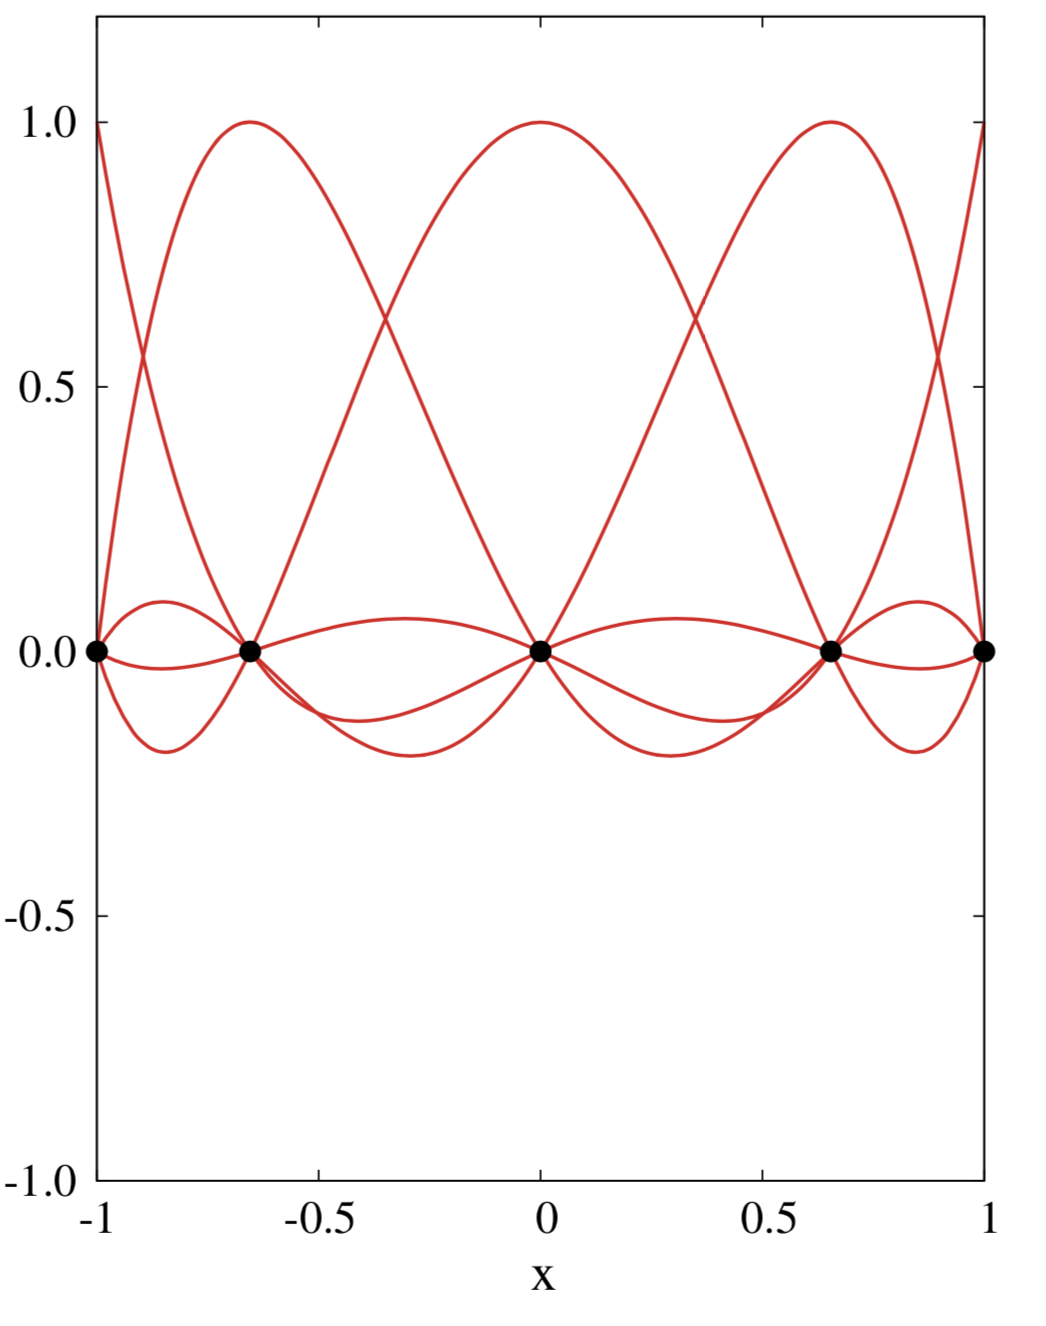
\includegraphics[width=0.4\textwidth]{CLIMA-numerics/figures/LGL-lagrange.png}
\caption{Basis functions of order 4 along the 1D reference element $\hat{e} = [-1,1]$. The black dotes are the non-equi-spaced Legendre–Gauss–Lobatto (LGL) quadrature points for this element.}
\label{fig:LGL}
\end{figure}

The space of tensor-product polynomials of degree $N$
is denoted as $\mathbb{Q}^{N}(\hat{e})$ where $\hat{e} = {[-1, 1]}^d$ is the reference element. In 3-D the solution inside the element is taken to be
\begin{align}
  \vec{Y}^{(e)}(\vec{\xi}, t) = \sum_{(i,j,k) = (0,0,0)}^{(N,N,N)}
  l_{i}(\xi_{1}) l_{j}(\xi_{2}) l_{k}(\xi_{3})
  \vec{Y}_{ijk}^{(e)}(t),
\end{align}
Here $l_{i}(\vec{x})$ are 1-D Lagrange polynomials associated with a set of
abscissae ${\{\hat{\xi}_{k}\}}_{k=0}^{N}$ (which should not be confused with
$\xi_{k}$ which is a component of $\vec{\xi}$). In terms of the physical
coordinate $\vec{x}$ the solution inside the element is then
\begin{align}
  \vec{Y}^{(e)}(\vec{\xi}^{(e)}(\vec{x}), t) = \sum_{(i,j,k) = (0,0,0)}^{(N,N,N)}
  l_{i}(\xi_{1}^{(e)}(\vec{x})) l_{j}(\xi_{2}^{(e)}(\vec{x}))
  l_{k}(\xi_{3}^{(e)}(\vec{x}))
  \vec{Y}_{ijk}^{(e)}(t).
\end{align}
Note that depending on the mapping $\vec{\xi}^{(e)}(\vec{x})$ the solution need
not be tensor product polynomial in the physical space.

\subsection{Quadrature and Variational Crimes (Brief Version)}
\label{aliasing_section}
We will use the same notation as \ref{illustrative_example}. The other thing that makes DG different from finite volume is \textbf{aliasing} issues.
Consider Burgers' equation, which is the nonlinear PDE
\begin{align}
    \partial_t \rho + \partial_x f &= 0 \\
    f &= \rho^2
\end{align}
In the Discontinuous Galerkin method all quantities are interpreted as belong to the polynomial basis set, including the flux term $f$, i.e., we represent our functions as
\begin{align}
    \rho &= \rho_i \ell_i \text{ and } 
    f = f_i \ell_i ,
\end{align}
which are polynomials of degree $N$, for $i = 0, ..., N$. But yet $f$ involves a \textit{product} of two polynomials of degree $N$, which is a polynomial of degree $2N$. This is not an issue in finite volume codes where $N = 0$ so that $2N = 0$, but can sometimes lead to issues in DG codes. This is the classic \textbf{closure problem} but in the context of numerical methods. 

Thus we must define in what sense we are representing a polynomial of degree $2N$ by a polynomial of degree $N$. We will discuss four (non-exhaustive) options
\begin{enumerate}
    \item Exact quadrature version 1
    \item Exact quadrature version 2
    \item Ignoring higher order terms, (Polynomials of Degree $N+1$ and higher) 
    \item Multiplying nodal points together
\end{enumerate}

\textbf{Exact quadrature version 1}: For exact quadrature we satisfy the nonlinear flux relation in the same sense that we are satisfying the PDE. We multiply through by test functions $\psi$ and integrate,
\begin{align}
\label{weak_form_nonlinear}
   \int_\Omega \psi f = \int_\Omega \psi \rho^2.
\end{align}
We represent functions as $f = f_j \ell_j$ and $\rho_j \ell_j$ so that \ref{weak_form_nonlinear} becomes
\begin{align}
    \int_\Omega \psi f_j \ell_j = \int_\Omega \psi \rho_j \ell_j \rho_k \ell_k.
\end{align}
We the take our test function space to be the same as our basis function space $\psi = \ell_i$ to get
\begin{align}
     \int_\Omega \ell_i  \ell_j f_j = \int_\Omega \ell_i  \ell_j  \ell_k \rho_j \rho_k.
\end{align}
The first term is just the entries of the mass matrix, i.e.,
\begin{align}
  \mathcal{M}_{ij}  =  \int_\Omega \ell_i  \ell_j ,
\end{align}
But for quadratic nonlinearities we need to compute integrals like
\begin{align}
\label{exact_quadrature_1}
   \mathcal{Q}^1_{ijk} \equiv \int_\Omega \ell_i(x) \ell_j(x) \ell_k(x)
\end{align}
which is a new object $\mathcal{Q}^1$. Thus we represent the equation as follows
\begin{align}
    \partial_t \mathcal{M}_{ij} \rho_j - \mathcal{S}_{ji} f_j &= \delta_{0i} f^*(x=-1,t) - \delta_{Ni} f^*(x=1,t) 
    \\
    \mathcal{M}_{ij} f_j &= \mathcal{Q}_{ijk}^1 \rho_j \rho_k
\end{align}
\textbf{Exact quadrature version 2}: This is similar to the previous one, except we directly represent the derivative term
\begin{align}
\label{exact_quadrature_2}
   \mathcal{Q}^2_{ijk} \equiv \int_\Omega \ell_i'(x) \ell_j(x) \ell_k(x)
\end{align}
so that the discrete equations are
\begin{align}
    \partial_t \mathcal{M}_{ij} \rho_j - \mathcal{Q}^2_{ijk} \rho_j \rho_k &= \delta_{0i} f^*(x=-1,t) - \delta_{Ni} f^*(x=1,t) 
\end{align}
\textbf{Ignoring higher order terms:} We carry through the multiplication of the polynomials, but just chop off all the terms corresponding to higher order terms. This can be done by ignoring higher Legendre modes (which is consistent with ``Exact Quadrature version 1") or by ignoring the monomial terms (which is not consistent with ``Exact Quadrature version 1"). 

\textbf{Multiplying nodal points together:} This is what is done in CLIMA. One perspective is that we are satisfying the equation
\begin{align}
    f_i \ell_i = (\rho_i \ell_i) (\rho_j \ell_j)
\end{align}
exactly at the nodal points. This leads to $f_j = (\rho_j)^2$. If we do so the we are mixing discretizations.
Another perspective is that we approximate ``exact quadrature version 1", \ref{exact_quadrature_1}, as
\begin{align}
   [\mathcal{Q}_1]_{ijk} \equiv \int_\Omega \ell_i(x) \ell_j(x) \ell_k(x) \approx \mathcal{M}_{ij} \delta_{jk}
\end{align}
so that $f_j = (\rho_j)^2$. This is also known as \textbf{inexact quadrature} or a \textbf{variational crime}. This approximation can lead to instability issues which are ameliorated either through dissipation, increasing resolution, or filters. When things are very resolved the higher order polynomial terms don't really play a role. This can either occur due $h$-refinement, since things are locally linear, or $p-$refinement for more complex reasons\footnote{The reasons are analagous to what happens with Fourier modes of analytic functions. Higher Fourier modes don't really matter since they decay exponentially and become negligible.}.

We now go through an explicit example of the differences for linear elements / polynomial order 1. Here the Lagrange interpolants are
\begin{align}
    \ell_0(x) = (x-1)/ (-2) \text{ and } \ell_1(x) = (x+1) / 2
\end{align}
We can perform all integrals from the previous section
\begin{align}
    \mathcal{Q}^1_{000} &= \mathcal{Q}^1_{111} =  1/2 \\
    \mathcal{Q}^1_{011} &= \mathcal{Q}^1_{101} = \mathcal{Q}^1_{110} = 1/6
    \\
    \mathcal{Q}^1_{100} &=
    \mathcal{Q}^1_{010} =
    \mathcal{Q}^1_{001} = 1/6
\end{align}
so that
\begin{align}
    \begin{bmatrix}
    2/3 & 1/3 \\
    1/3 & 2/3
    \end{bmatrix}
    \begin{bmatrix}
    f_0 \\
    f_1
    \end{bmatrix}
    &= 
        \begin{bmatrix}
    1/2 & 1/3 & 1/6 \\
    1/6 & 1/3 & 1/2
    \end{bmatrix}
        \begin{bmatrix}
    (\rho_0)^2 \\
    \rho_0 \rho_1 \\
    (\rho_1)^2
    \end{bmatrix}
\end{align}
which is 
\begin{align}
        \begin{bmatrix}
    f_0 \\
    f_1
    \end{bmatrix}
    &= 
        \begin{bmatrix}
    5/6 & 1/3 & -1/6 \\
    -1/6 & 1/3 & 5/6
    \end{bmatrix}
        \begin{bmatrix}
    (\rho_0)^2 \\
    \rho_0 \rho_1 \\
    (\rho_1)^2
    \end{bmatrix}
\end{align}
For the other operator we have
\begin{align}
    \mathcal{Q}^2_{000} &= [\mathcal{Q}_2]_{011} = -1/3 
    \\
    \mathcal{Q}^2_{010} &= \mathcal{Q}^2_{001} = -1/6 
    \\
    \mathcal{Q}^2_{1ij} &= -[\mathcal{Q}_2]_{0ij}  
\end{align}
Note that $\mathcal{S}_{ji}\mathcal{Q}^1_{jks} = \mathcal{Q}^2_{iks}$. The two ``exact quadrature" versions coincide for linear elements.

Now let us check to see what it means to lop off higher  order terms
\begin{align}
    4 \rho^2 &= 4 \left(\rho_0 \frac{x-1}{-2} + \rho_1 \frac{x+1}{2} \right)^2
    \\
    &= (\rho_0^2 + \rho_1^2 - 2 \rho_0 \rho_1) x^2
    + 2(\rho_0^2 - \rho_1^2)x + (\rho_0^2 + \rho_1^2 + 2 \rho_0 \rho_1)
    \\
    \label{polynomial_explicit}
    &= (\rho_0 - \rho_1)^2 x^2 
    + (3 \rho_0^2 - \rho_1^2 + 2\rho_0 \rho_1 )\frac{x-1}{-2} + (3 \rho_1^2 - \rho_0^2 + 2 \rho_0 \rho_1)\frac{x+1}{2}
\end{align}
In this case we just neglect the term in front of $x^2$. Thus $f$ becomes
\begin{align}
        \begin{bmatrix}
    f_0 \\
    f_1
    \end{bmatrix}
    &= 
        \begin{bmatrix}
    3/4 & 1/2 & -1/4 \\
    -1/4 & 1/2 & 3/4
    \end{bmatrix}
        \begin{bmatrix}
    (\rho_0)^2 \\
    \rho_0 \rho_1 \\
    (\rho_1)^2
    \end{bmatrix}
\end{align}
If we had instead decided to take off the highest Legendre modes (as opposed to highest polynomial order), then we should reduce back to the exact quadrature formula (version 1). To see this first note that the first few legendre polynomials are
\begin{align}
    P_0(x) = 1 \text{ , } P_1(x) = x  \text { , and } P_2(x) = \frac{3}{2} \left(x^2 - \frac{1}{3} \right)
\end{align}
Thus if we rewrite \ref{polynomial_explicit} with the highest polynomial order instead represented instead with Legendre modes via $x^2 = x^2 - 1/3 + 1/3 = 2/3 P_2(x) + 1/3$, then we get 
\begin{align}
    \label{polynomial_explicit_legendre}
    4 \rho^2 &= 
    (\rho_0 - \rho_1)^2 (x^2-1/3+1/3) 
    \\
    &+ (3 \rho_0^2 - \rho_1^2 + 2\rho_0 \rho_1 )\frac{x-1}{-2} + (3 \rho_1^2 - \rho_0^2 + 2 \rho_0 \rho_1)\frac{x+1}{2}
    \\
    &= (\rho_0 - \rho_1)^2 \frac{2}{3} P_2(x)
    \\
    &+ \left(\frac{10}{3} \rho_0^2 - \frac{2}{3}\rho_1^2 + \frac{4}{3} \rho_0 \rho_1 \right)\frac{x-1}{-2} + \left(\frac{10}{3} \rho_1^2 - \frac{2}{3} \rho_0^2 + \frac{4}{3} \rho_0 \rho_1  \right)\frac{x+1}{2}
\end{align}
Neglecting the higher order Legendre modes (in this case just $P_2(x)$, but in general much more). We indeed get (upon dividing by 4)
\begin{align}
        \begin{bmatrix}
    f_0 \\
    f_1
    \end{bmatrix}
    &= 
        \begin{bmatrix}
    5/6 & 1/3 & -1/6 \\
    -1/6 & 1/3 & 5/6
    \end{bmatrix}
        \begin{bmatrix}
    (\rho_0)^2 \\
    \rho_0 \rho_1 \\
    (\rho_1)^2
    \end{bmatrix}
\end{align}
as before.

And the last option is to represent $f_0$ and $f_1$ as
\begin{align}
        \begin{bmatrix}
    f_0 \\
    f_1
    \end{bmatrix}
    &= 
        \begin{bmatrix}
    1 & 0 & 0 \\
    0 & 0 & 1
    \end{bmatrix}
        \begin{bmatrix}
    (\rho_0)^2 \\
    \rho_0 \rho_1 \\
    (\rho_1)^2
    \end{bmatrix}
\end{align} 
as is done in the CLIMA code. Again this just corresponds to multiplying things nodally, point by point. 

\subsection{Topography/Bathymetry}
Topography can be either built analytical or by reading an external topography file. The topography data are taken from the NOAA ETOPO-1 database \cite{etopo1}. As of now, only {\bf XYZ files are being read}. If necessary, a NetCFD topograpjhy reader can be easily added.
An example of high order grid built on the topography of the Monterey bay in California is shown in Figure \ref{fig:montereySurfaceGrid}. The high order grid is built so that the elements follow the geometric curvature. A detailed view of the curved high order elements is shown in Figure \ref{fig:gridDetailView}
%FIGURE COMMENT HERE
% \begin{figure}[htbp]
% \centering
% 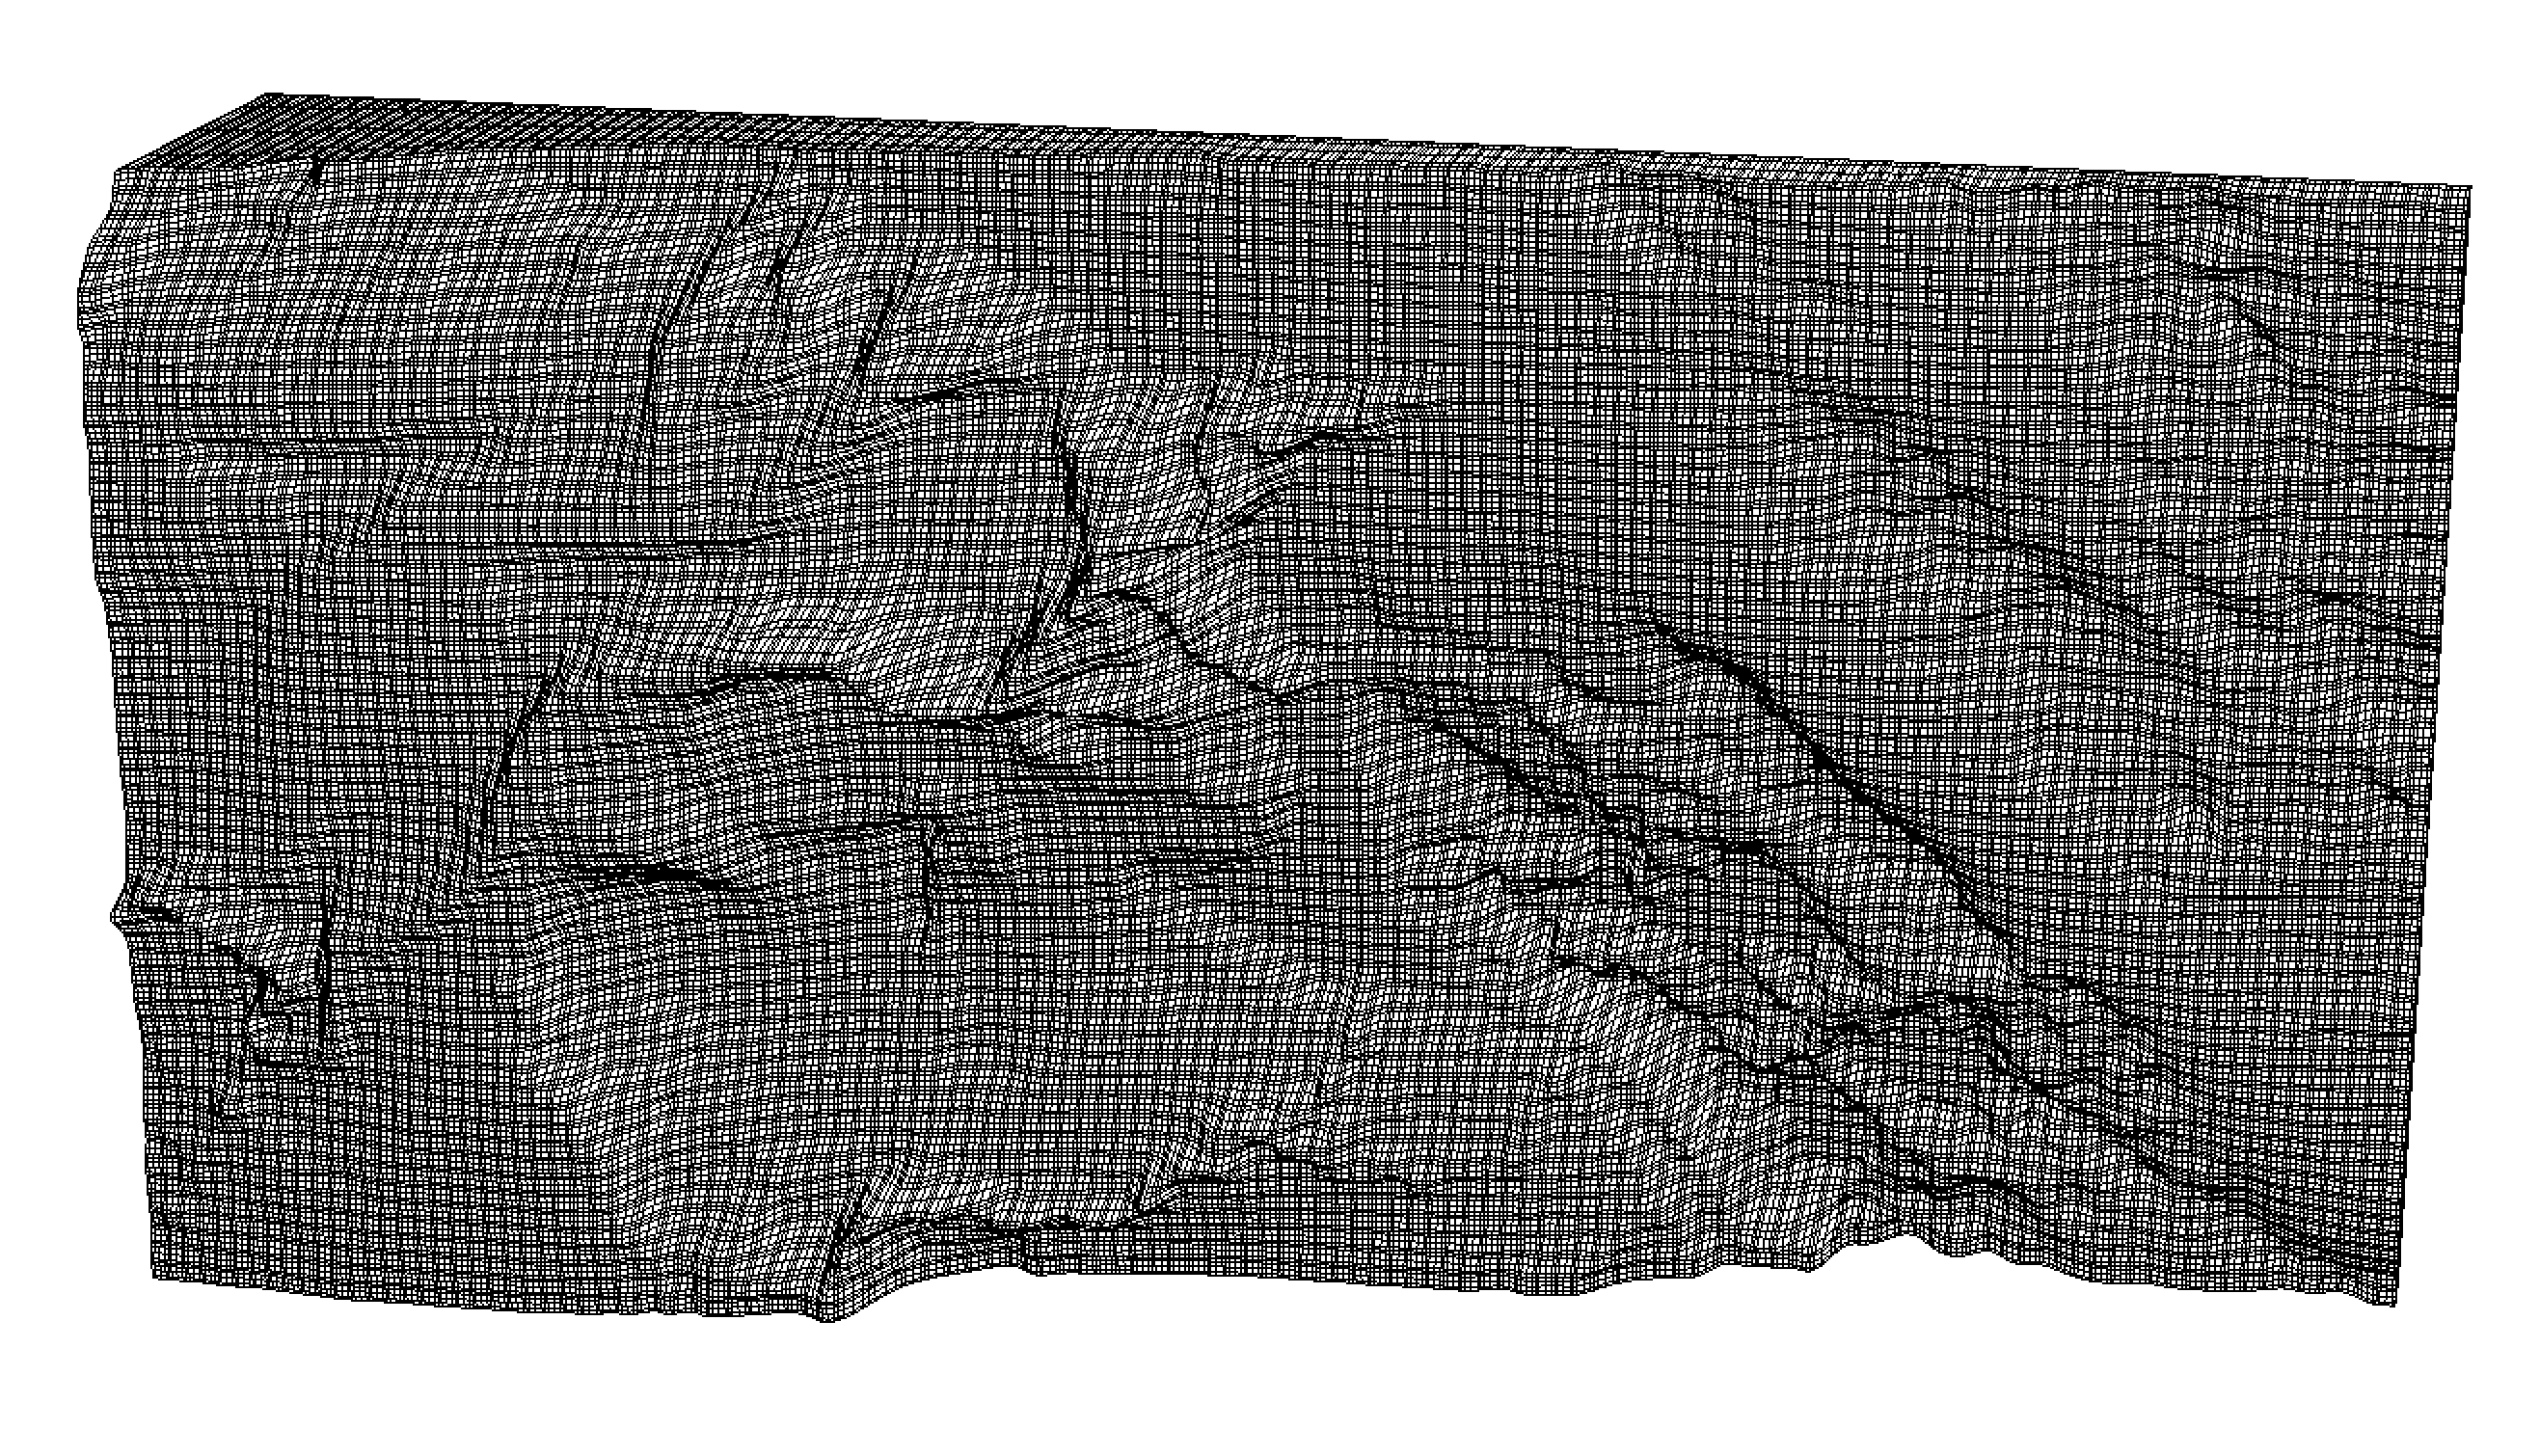
\includegraphics[width=\textwidth]{figures/monterey_with_grid.png}
% 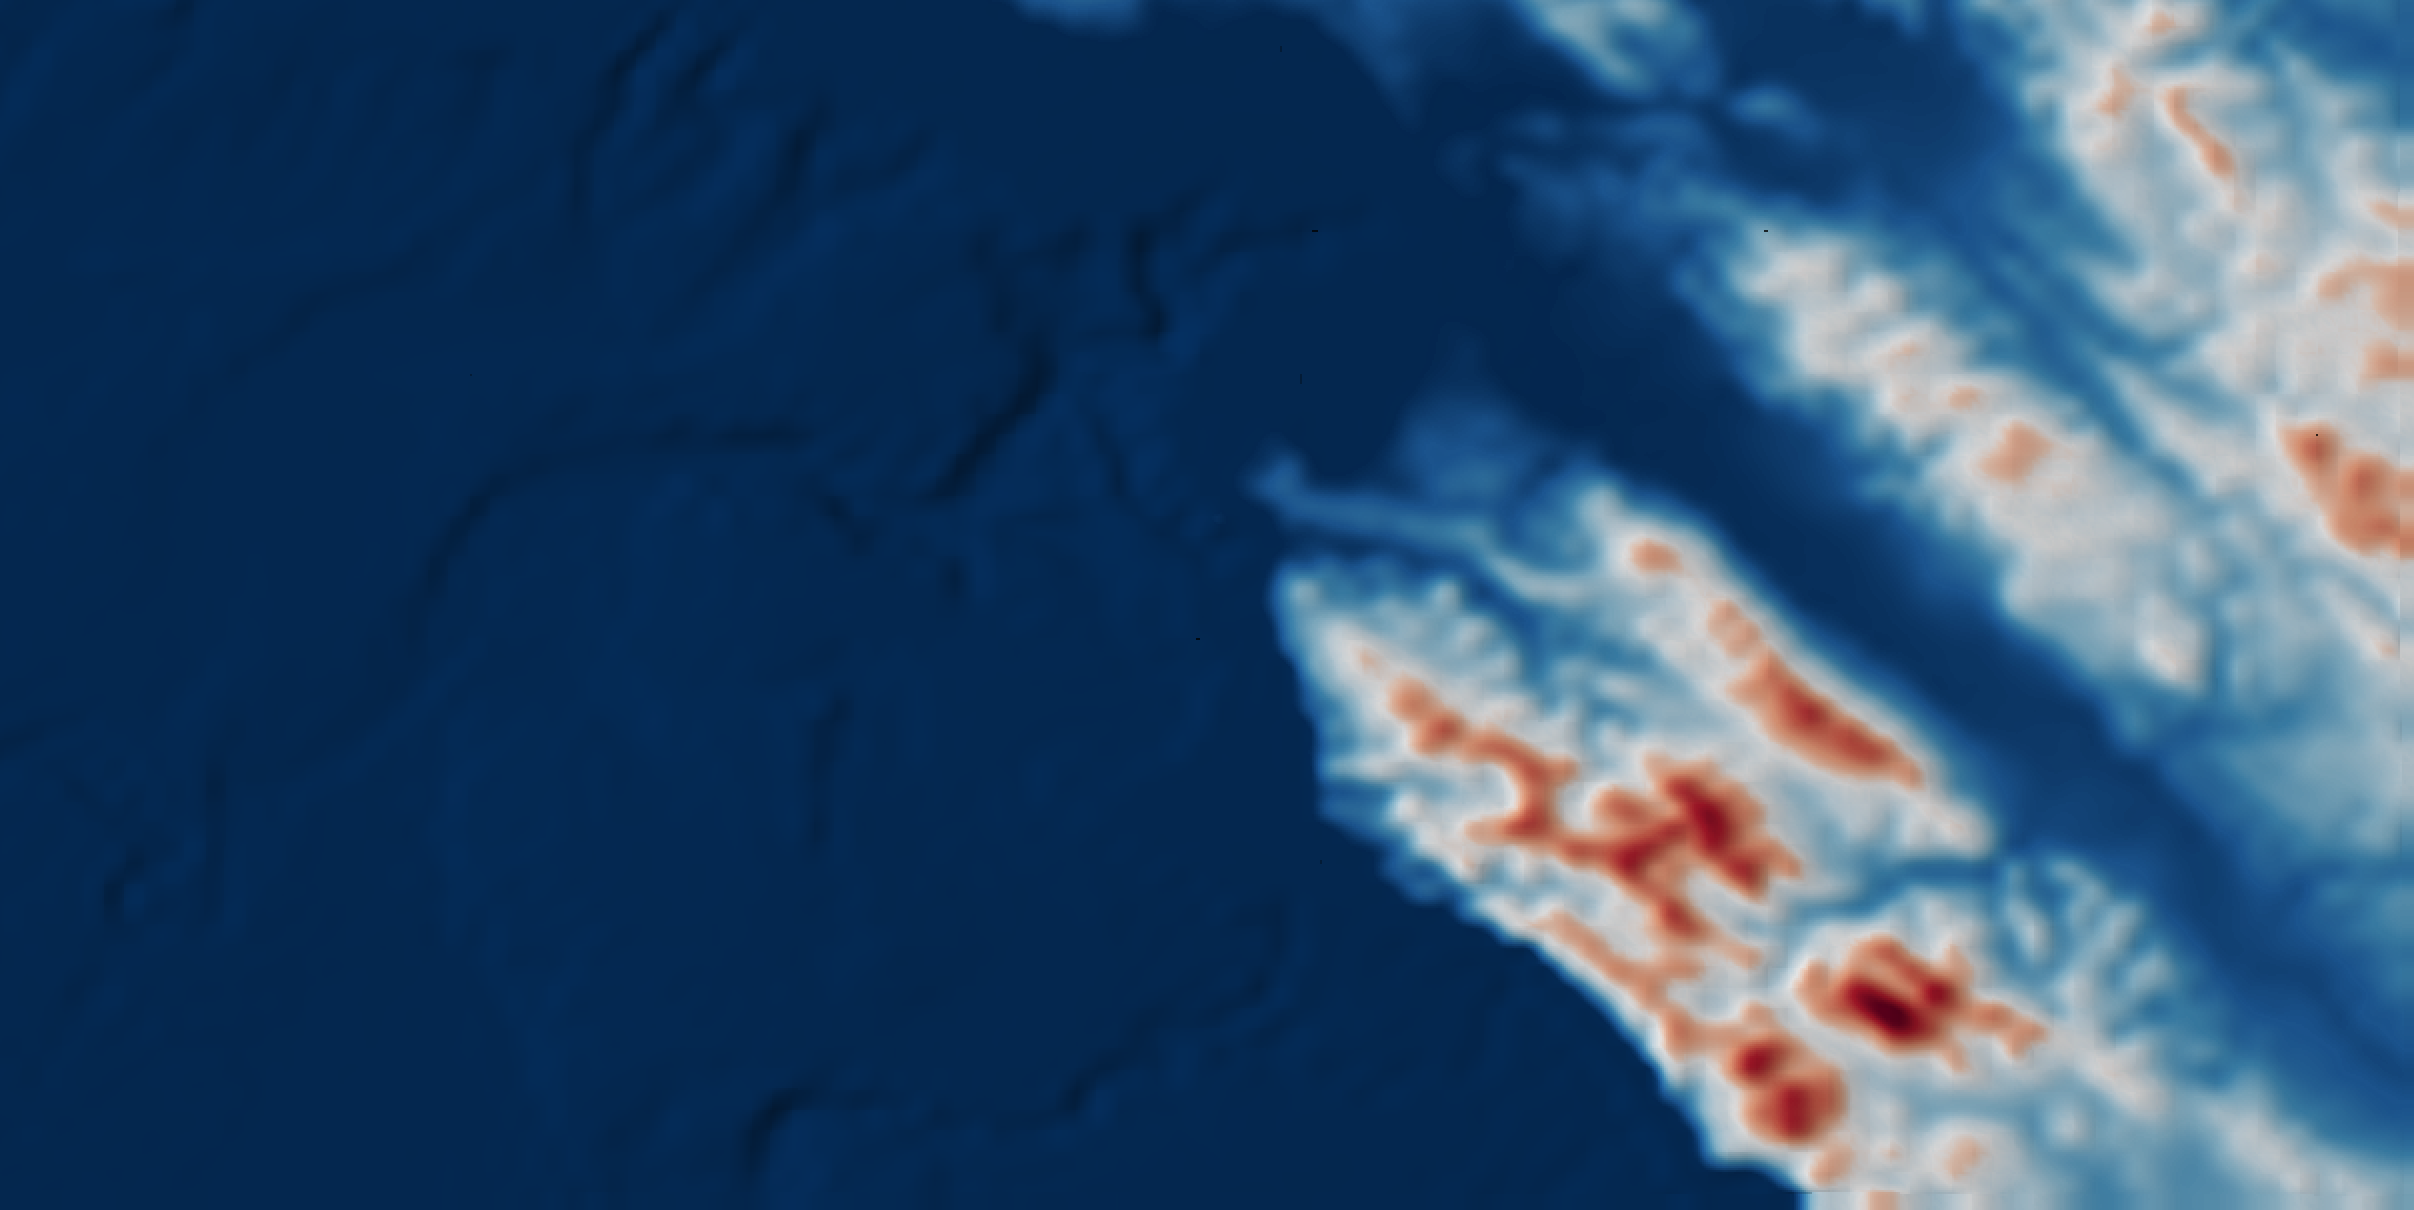
\includegraphics[width=\textwidth]{figures/monterey_colorscale.png}
% \caption{Bottom view of the meshed Monterey Bay, California. The high order elements are visible in the top image whereas the topography is colored by its elevation in the bottom.}
% \label{fig:montereySurfaceGrid}
% \end{figure}

% \begin{figure}[htbp]
% \centering
% 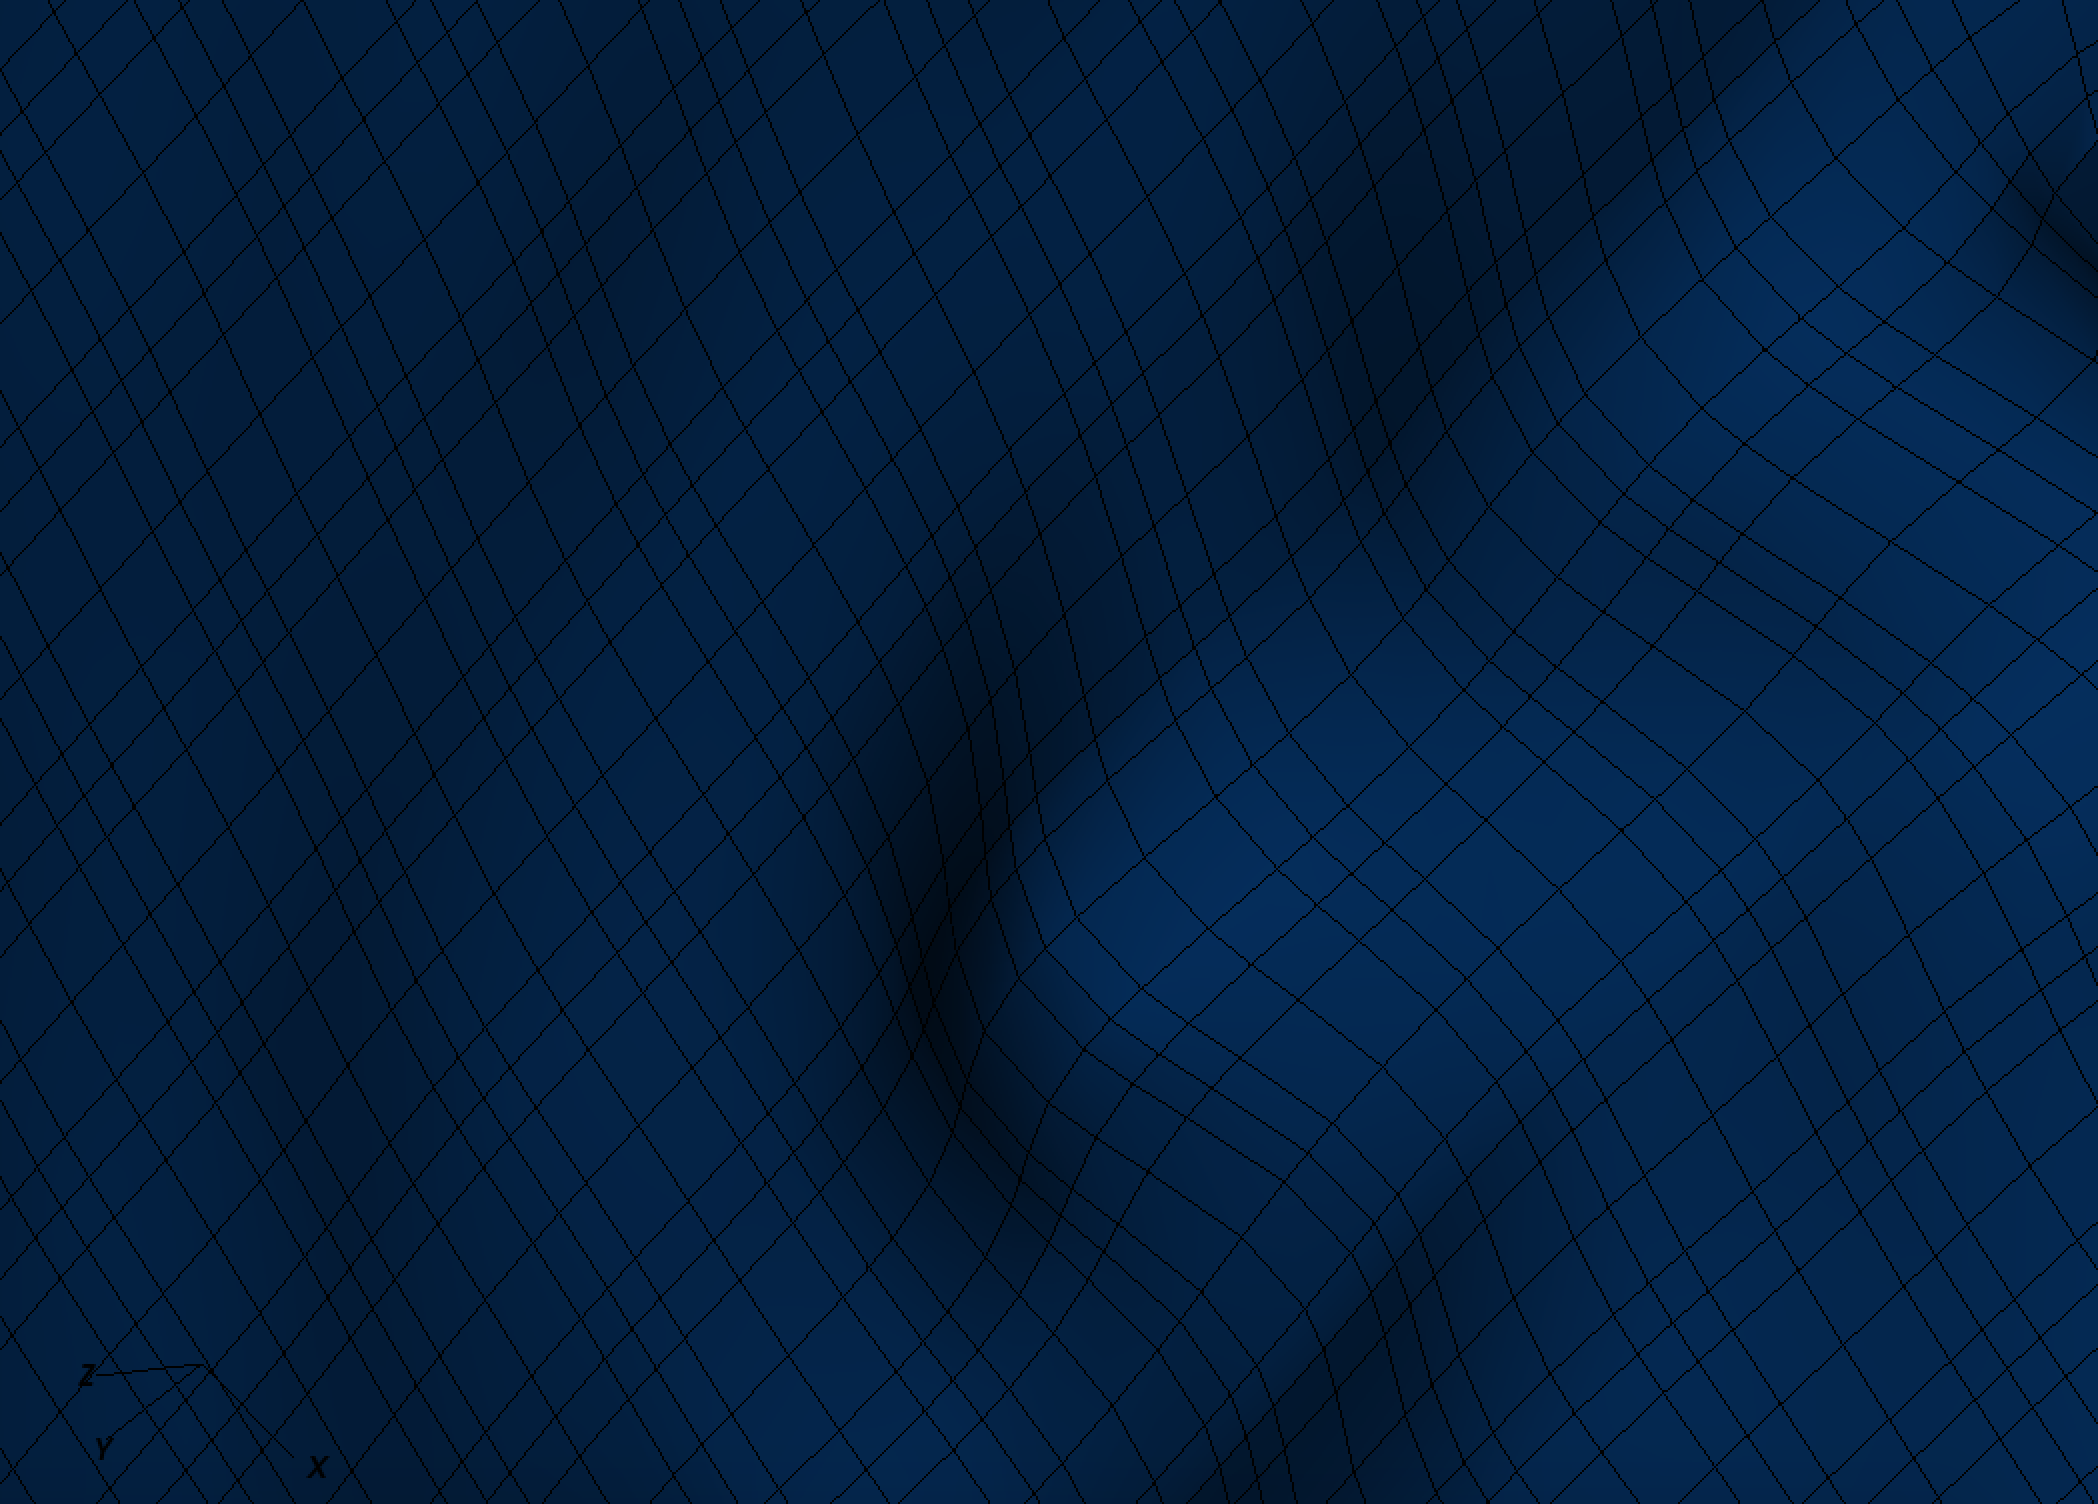
\includegraphics[width=\textwidth]{figures/GRID-detail.png}
% \caption{A close view of the curved high order elements on the topography.}
% \label{fig:gridDetailView}
% \end{figure}

\subsubsection{Topography/Bathymetry Files and Database}
The external topographic files are not incorporated into the CLIMA repository. 
They are automatically downloaded via a call to {\tt wget} from the {\tt Julia} driver into the user's working directory {\tt \$CLIMA\_HOME/USERS/TEST/DIRECTORY}. As of now, the available topography files are hosted here \url{https://web.njit.edu/~smarras/TopographyFiles} (notice: this directory is not directly accessible from the browser).

\subsection{Horizontal-Vertical Splitting}
Let denote the transform between any reference coordinate system~$(\alpha, \beta, \xi)$ to the physics computational domain
$$\bm{r} = (x, y, z) := G(\alpha, \beta, \xi, t) $$
, where $\xi \in [0,1]$ corresponds to the radial direction. The radius $r=r(\alpha,\beta,\xi, t)$ satisfies that $r(\alpha, \beta, 0, t)$ is coincident with the surface and $r(\alpha, \beta, 1, t)$ is coincident with the top. 
The contravariant bases in the physics computational domain are 
$$\bm{g}_{\alpha} = \frac{\partial \bm{r}}{\partial \alpha},\,\bm{g}_{\beta} = \frac{\partial \bm{r}}{\partial \beta},\,\textrm{and},\,\bm{g}_{\xi} = \frac{\partial \bm{r}}{\partial \xi}$$
It is worth mentioning these bases are time dependent.

The vertical velocity is $w = \frac{Dr}{Dt}$ (\ht{material derivative}). And the coordinate velocity of $\xi$ is $u^{\xi}$ (\hl{flow velocity in this coordinate}).
The relation between $w$ and $u^{\xi}$ is
\begin{align*}
    &w = \frac{Dr}{Dt} = \frac{\partial r}{\partial t} + \frac{\partial r}{\partial \alpha} u^{\alpha} +  \frac{\partial r}{\partial \beta} u^{\beta} + \frac{\partial r}{\partial \xi} u^{\xi} \\
    &u^{\xi}(w, u^{\alpha}, u^{\beta}) = \Big(\frac{\partial r}{\partial \xi}\Big)^{-1}(w - \frac{\partial r}{\partial \alpha} u^{\alpha} -  \frac{\partial r}{\partial \beta} u^{\beta}  )
\end{align*}
where the flow velocity is $\bm{u} = u^{\alpha}\bm{g}_{\alpha} + u^{\beta}\bm{g}_{\beta} + u^{\xi}\bm{g}_{\xi}$. It worth mentioning for spherical coordinates and without topography, $\frac{\partial r}{\partial \alpha} = 0 $ and $\frac{\partial r}{\partial \beta} = 0$.

The mass conservation equation becomes
\begin{align*}
    &\frac{\partial \rho}{\partial t} + \nabla (\bm{u}\rho) = 0 \\
    &\frac{\partial \rho}{\partial t}  + \frac{1}{J} \frac{\partial }{\partial \alpha} (\rho u^{\alpha}) + \frac{1}{J} \frac{\partial }{\partial \beta} (\rho u^{\beta}) + \frac{1}{J} \frac{\partial }{\partial \xi} (\rho u^{\xi}) = 0
\end{align*}
The momentum conservation equation is
\begin{align*}
    &\frac{\partial \rho \vec{u}}{dt} + \nabla \Big(\rho \bm{u} \otimes \bm{u} + pI\Big) + f\rho \bm{k}\times \bm{u} = 0 \\
\end{align*}
The integration form in physical domain $\Omega(\alpha, \beta, \xi, t)$ is 
\begin{align*}
    &\int_{\Omega} \frac{\partial \rho \vec{u}}{dt} + \int_{\partial \Omega} \Big(\rho \bm{u} \otimes \bm{u} + pI\Big) \cdot \bm{n} + \int_{\Omega} f\rho\bm{k}\times \bm{u} = 0 \\
\end{align*}

\begin{align*}
    &\frac{\partial}{\partial t} \int_{\Omega} \rho \vec{u} - \int_{\partial \Omega} \rho \vec{u} (\nu_G \cdot \bm{n}) + \int_{\partial \Omega} \Big(\rho \bm{u} \otimes \bm{u} + pI\Big) \cdot \bm{n} + \int_{\Omega} f\rho\bm{k}\times \bm{u} = 0 \\
\end{align*}


\begin{align*}
    &\frac{\partial}{\partial t} \int_{\Omega_0} |J|\rho \vec{u} + \int_{\partial \Omega_0} \Big(\rho \bm{u} \otimes (\bm{u} - \nu_G) + pI\Big) \cdot |J|J^{-T}\bm{N} + \int_{\Omega_0} |J|f\rho\bm{k}\times \bm{u} = 0 \\
\end{align*}

\ht{Since these bases} $\bm{e}_{\alpha}$ might depend on $t$, 
\begin{align*}
    &\frac{\partial u^{\alpha}}{\partial t} + u^{i} \nabla_i u^{\alpha} + \theta g^{\alpha i} \nabla_i \Pi + f(k\times \vec{u})^{\alpha} = 0 \\
\end{align*}

\section{Still TODO:}
\begin{itemize}
  \item Bring code in line with skew symmetric formulation
  \item Replace in code \texttt{diffusive\_penalty!} with
    \texttt{gradient\_numerical\_flux!}
  \item Check / correct boundary conditions already in use in the code
  \item Add more BC types?
  \item Add details on BCs for moisture / tracer variables
  \item Add DG refs (skew symmetric formulation stuff, geometry handling, etc.)
\end{itemize}

\hl{The grid reader should be enhanced to map the grid onto the sphere. As of now, the grid is read and mapped into a closed box only.}


\chapter{Time Discretization}\label{s:timestepping}

The general, compressible equations of motion we use permit a variety of wave modes with different characteristic speeds. Additionally, the equations contain sources that can add stiffness, for example, microphysical processes that occur on timescales of seconds or less.

The equations permit the following wave modes:
\begin{itemize}
    \item Acoustic waves. They have phase speeds around $300~\mathrm{m~s^{-1}}$ in the atmosphere. Density variations and the terms involving pressure in the momentum and energy equations are essential for their existence.
    \item Gravity waves. They have a spectrum of phase speeds. In a deep atmosphere (e.g., in a GCM), the gravest, external mode has phase speed $(gH)^{1/2} \approx 280~\mathrm{m~s^{-1}}$, where $H\approx 8~\mathrm{km}$ is the atmospheric scale height. The gravity term $-\rho \nabla \Phi$ in the momentum equation and the gravitational potential energy $\Phi$ in the energy equation are responsible for their existence.
    \item Inertia-gravity, Rossby waves, and several other wave modes that owe their existence to the Coriolis acceleration $-2\vec{\Omega} \times \rho \vec{u}$. They have smaller phase speeds than the acoustic and external gravity waves.
\end{itemize}
Additional stiffness in the equations arises from:
\begin{itemize}
    \item Falling precipitation, whose fall velocity $w_{p,i}$ can reach $10~\mathrm{m~s^{-1}}$ and thus exceeds typical vertical velocities resolved in GCMs.
    \item Microphysical source terms, for example, in the equations for suspended specific humidities $q_k$; they depend on the precipitation specific humidity $q_{p,i}$, which can change rapidly because precipitate falls rapidly. 
    \item SGS diffusive fluxes, whose effective vertical velocity can exceed that of the resolved velocities.
    \item Other parameterized SGS fluxes, for example, convective updrafts, whose vertical velocities can likewise be large.
\end{itemize}
By contrast, radiation evolves on longer timescales than the dynamical quantities and hence, because it is expensive to evaluate, usually is evolved forward in time with longer timesteps than the dynamical quantities. 

We need a stable and computationally efficient time discretization strategy that allows some state vector components to be subcycled several times per dynamical timestep (e.g., $q_{p,i}$ and convective updrafts) and allows some rapidly evolving source/sink terms (e.g., from microphysics) to be accumulated over the subcycled timesteps. At the same time, it should allow other terms (e.g., radiative energy fluxes) to be evaluated less frequently. In particular, we need a computationally efficient way of handling the physically insignificant acoustic waves.
     
\section{Decomposition of Time Tendencies}

To circumvent the time-step restriction due to the fast acoustic and gravity waves, using implicit-explicit (IMEX) methods is one option. For the LES model, if the aspect ratio of the horizontal ($\Delta_h$) to vertical ($\Delta_v$) grid spacing is near unity, using fully 3D-IMEX methods may be an option.  For LES models with aspect ratios of grid elements $\Delta_h/\Delta_v > 1$ and for global atmospheric models, which generally have $\Delta_h/\Delta_v \gg 1$, we use 1D-IMEX methods in which the time-integrator is fully explicit in the horizontal direction (HE) and implicit in the vertical direction (so-called HEVI schemes). 

IMEX methods require the solution of one or more linear systems at each time step. The linear system is global in 3D, and this may limit scalability of IMEX methods in a multi-node computational setting. In that case, split-explicit methods may be a more scalable option to deal with the timestep restrictions. For HEVI schemes, the linear solves are restricted to independent atmospheric columns, which are represented on a single compute node (if the domain decomposition is done in the horizontal). So their scalability across nodes is less restricted.

All of these approaches are based on a decomposition of the total tendency $\vec{\mathcal{T}}$ on the right-hand side of Eq.~\eqref{e:eom_compact} into four terms: 
\begin{itemize}
    \item terms to be treated implicitly, labeled by $I$ (the fastest terms);
    \item terms evaluated at the dynamical (advective) timestep, labeled by $d$;
    \item terms to be subcycled $f$ times for each dynamical timestep, labeled by $+f$ (for fast);
    \item terms to be evaluated every $s$ dynamical timesteps, labeled by $-s$ (for slow).
\end{itemize}
This gives
\[
\frac{\partial \vec{Y}}{\partial t} = \Tvector = - \nabla \cdot \Fvector + \vec{\mathcal{S}} = \Tvector_{I} + \Tvector_{d} + \Tvector_{+f} + \Tvector_{-s}.
\]
To obtain a linear problem for the implicit solve, let us linearize the implicit tendency terms $\Tvector_{I}$ by Taylor expansion around a reference state $\vec{Y}_r$,
\begin{equation}\label{e:imex_linearization}
\Tvector_{I}(\vec{Y}) =  \Tvector_I(\vec{Y}_r) + \vec{\mathcal{L}}_I (\vec{Y} - \vec{Y}_r) + \Tvector^N_{I}(\vec{Y}),
\end{equation}
where 
\begin{equation}
    \vec{\mathcal{L}}_I = \left. \frac{\partial\Tvector_I}{\partial\vec{Y}}\right|_{\vec{Y}_r}
\end{equation} 
is the linear component of the tendency operator and $\Tvector^N_{I}(\vec{Y})$ is the nonlinear residual. This then allows us to write the equation of motion \eqref{e:eom_compact} as
\begin{equation}
\label{eq:IMEX}
\frac{\partial\vec{Y}}{\partial t} =  \vec{\mathcal{L}}_I \vec{Y} + \Bigl(\Tvector_I(\vec{Y}_r) - \vec{\mathcal{L}}_I \vec{Y}_r\Bigr) + \Tvector^N_{I}(\vec{Y}) + \Tvector_{d} + \Tvector_{+f} + \Tvector_{-s}.
\end{equation}
Usually, the reference state $\vec{Y}_r$ is chosen so that the tendency of the reference state, $\Tvector_I(\vec{Y}_r)$, and the linear tendency of the reference state, $\vec{\mathcal{L}}_I \vec{Y}_r$, either vanish individually or cancel each other, so that $\Tvector_I(\vec{Y}_r) - \vec{\mathcal{L}}_I \vec{Y}_r=0$. We will justify this in section~\ref{s:IMEX_general}.

\section{Reference State for Linearization}

Solving for the fastest waves implicitly by a linear solve requires linearization of the fastest tendency terms. We generally use reference states characterized by a temperature $T_r(z)$ that may depend on height $z$ but does not depend on horizontal coordinates or time. We enforce hydrostatic balance, and assume the reference state is dry.
%so that the reference state variables are obtained as described in section~\ref{s:initial_conditions} with zero relative humidity ($\mathrm{RH}=0$): the pressure is obtained from \eqref{eq:hydro_pressure}, the density from \eqref{eq:hydro_density}, and the total specific humidity is set to zero, $q_{t,r}=0$.

Because the reference temperature and thus the reference pressure are assumed to be constant in the horizontal, the reference state is assumed at rest, $\vec{u}_r = 0$, consistent with geostrophic balance. Because the reference state is assumed dry, $q_k= 0$ for $k \in \{ t, v, l, i, p\}$ in the reference state.

More sophisticated reference states for linearization are possible, for example, with a latitudinally varying hydrostatically balanced temperature profile, and with a reference velocity in geostrophic and hydrostatic balance with this temperature field. However, we focus on hydrostatic states at rest for now. 
 
 \section{Solving for Acoustic and Gravity Waves Implicitly}
 \label{s:IMEX_general}

Let us lay out in general terms the linearizations for acoustic and gravity waves that underlie IMEX methods in 1D and 3D. The tendency terms responsible for acoustic waves and gravity waves are
 \begin{equation}
 \Tvector_{I}= -\nabla_{1/3} \cdot
 \begin{pmatrix}
 \rho \vec{u} \\
 p \vec{I}_3 \\
 \bigl(e^{\mathrm{tot}} + (\delta_{\mathrm{gw}}-1) \Phi + p/\rho \bigr) \rho \vec{u} \\
 0\\
 \vdots
 \end{pmatrix}
 - \begin{pmatrix}
 0 \\
 \delta_{\mathrm{gw}} \rho \nabla_{1/3} \Phi \\
 0\\
 0\\
 \vdots
 \end{pmatrix},
 \label{eq:3d-imex/tendencies}
 \end{equation}
where all components indicated by dots are zero. The operator $\nabla_{1/3}$ is the 3D differential operator $\nabla_3 = \nabla$ for 3D-IMEX, and it is the 1D operator $\nabla_1 = \vec{k} \partial/\partial_z$ for 1D-IMEX. (The geopotential gradient $\nabla_{1/3} \Phi$ only has a vertical component as long as we consider a spherical planet, so this gradient even in 3D usually only has a vertical component.) The switch $\delta_{\mathrm{gw}}$ (which can only take the value of either $0$ or $1$) is included to indicate whether gravity waves are included in the implicit tendencies: 
\begin{itemize}
    \item $\delta_{\mathrm{gw}}=1$: both acoustic and gravity waves are included in $\Tvector_I$;
    \item $\delta_{\mathrm{gw}}=0$: only acoustic waves are included in $\Tvector_I$.
\end{itemize}

In the tendency \eqref{eq:3d-imex/tendencies}, the terms that need to be linearized are the pressure $p$, which depends nonlinearly on state variables, and the total enthalpy flux $(\rho e^{\mathrm{tot}} + p/\rho) (\rho \vec{u})$. Linearization around a state of rest ($\vec{u}_r=0$) with reference total energy $e^{\mathrm{tot}}_r$, pressure $p_r$, and density $\rho_r$ leads to
 \begin{equation}\label{e:IMEX_linear}
 \vec{\mathcal{L}}_I \vec{Y} = 
 -\nabla_{1/3} \cdot \begin{pmatrix}
 \textcolor{blue}{\rho \vec{u}} \\
 \textcolor{blue}{p_L} \vec{I}_3  \\
 \Bigl(e^{\mathrm{tot}}_r  + (\delta_{\mathrm{gw}}-1)\Phi + p_r/\rho_r \Bigr) \textcolor{blue}{\rho \vec{u}}\\
 0\\
\vdots
\end{pmatrix}
-
\begin{pmatrix}
0 \\
\delta_{\mathrm{gw}} \textcolor{blue} \rho \nabla_{1/3} \Phi \\
0\\
0\\
\vdots
\end{pmatrix}.
\end{equation}
This is linear with respect to \textcolor{blue}{$\rho$} and \textcolor{blue}{$\rho \vec{u}$} (all state variables and linear functions thereof are colored \textcolor{blue}{blue}; all other terms are constants or fixed functions of height $z$). For it to be a linear function of all state variables, the pressure \textcolor{blue}{$p_L$} needs to be expressed as a linear function of state variables. To derive a linear approximation for the pressure, we use the ideal gas law $p = R_m (\rho T)$ and the expression derived from the temperature equation 
%Eq.~\eqref{eq:temperature} 
for $\rho T$ in terms of the internal energy and specific humidities,
\begin{equation}\label{e:pressure}
\begin{split}
p &= R_m (\rho T) \\
  &= \rho R_m T_0 + \frac{R_m}{c_{vm}} \left[\rho e^{\mathrm{tot}} - \rho \Phi - 0.5 \rho \|\vec{u}\|^2 - (\rho q_t - \rho q_l) I_{v,0} + \rho q_i (I_{i,0} + I_{v,0}) \right],
\end{split}
\end{equation}
where we have used the relation $I = e^{\mathrm{tot}} - \Phi - 0.5 \|\vec{u}\|^2$ between total and internal energy. Linearization $p_L = p_r + (\partial p/\partial\vec{Y})\cdot(\vec{Y}-\vec{Y}_r)$ around the reference state $\vec{Y}_r$ with pressure $p_r$ and zero specific humidities leads to 
\begin{equation}\label{eq:pressure_linear}
\textcolor{blue}{p_L} = \textcolor{blue}{\rho} R_d T_0 + \frac{R_d}{c_{vd}} \bigl[ \textcolor{blue}{\rho e^{\mathrm{tot}}} - \textcolor{blue}{\rho} \Phi - (\textcolor{blue}{\rho q_t} - \textcolor{blue}{\rho q_l})I_{v,0} + (\textcolor{blue}{\rho q_i}) (I_{i,0} + I_{v,0}) \bigr].
\end{equation}
If only the total specific humidity $q_t$ is available as a prognostic variable and condensate is determined by saturation adjustment, the condensate specific humidities $q_l$ and $q_i$ in this linearized expression for the pressure can be set to zero. Note that the temperature $T_0$ that appears here is the \emph{reference temperature in the definition of internal energy}, a model constant; it is \emph{not} the temperature $T_r$ of the reference state about which we linearized. In fact, the linearized pressure \eqref{eq:pressure_linear} does not depend on the reference state: the zeroth-order term $p_r$ in the linearization cancels the terms involving the reference state in the linear term, which ensures that the linearized pressure vanishes when the density vanishes. 

We can now see that the sum of the terms involving the reference state in the decomposition \eqref{e:imex_linearization} vanishes,
\[
\Tvector_I(\vec{Y}_r) - \vec{\mathcal{L}}_I \vec{Y}_r = 0.
\]
To see this, it is useful to distinguish the cases when gravity waves are included in the implicit term and when they are not included: 
\begin{itemize}
    \item Acoustic and gravity waves included ($\delta_{\mathrm{gw}}=1$). In this case, it is evident that $\Tvector_I(\vec{Y}_r)=0$ because the pressure gradient ($-\nabla_{1/3} p_r(z)$) and geopotential gradient ($-\rho_r\nabla_{1/3}\Phi$) in the momentum equation (second component of tendency vector) cancel for a hydrostatic reference state with $p_r = p_r(z)$. The same is true for the linear term for a reference state at rest, for which $p_L = p_r$ and $\vec{\mathcal{L}}_I \vec{Y}_r = 0$. 
    \item Only acoustic waves included ($\delta_{\mathrm{gw}}=0$). In this case, neither $\Tvector_I(\vec{Y}_r)$ nor $\vec{\mathcal{L}}_I\vec{Y}_r$ vanish individually, because the geopotential term needed for the cancellation of terms in hydrostatic balance does not appear in the momentum tendency. However, $p_L = p_r$ in a reference state at rest, so that $\Tvector_I(\vec{Y}_r) = \vec{\mathcal{L}}_I\vec{Y}_r$.
\end{itemize}
Thus, in either case, the terms involving the reference state do not appear  in the decomposition \eqref{e:imex_linearization}. 

The nonlinear term follows as the residual 
\begin{equation}\label{e:nonlinear_residual}
\begin{split}
\Tvector^N_{I}(\vec{Y}) & =  \Tvector_I(\vec{Y}) - \vec{\mathcal{L}}_I \vec{Y} \\
& = 
-\nabla_{1/3} \begin{pmatrix}
0 \\
(p - p_L) \vec{I}_3\\
(e^{\mathrm{tot}}  + p/\rho - e^{\mathrm{tot}}_r - p_r/\rho_r) \rho \vec{u}\\
0\\
\vdots
\end{pmatrix}.
\end{split}
\end{equation}
We can verify that the nonlinear residual is small relative to the linear tendency term, as is required for an IMEX approach, as follows. The full pressure (Eq.~\ref{e:pressure}) differs from its linearized counterpart (Eq.~\ref{eq:pressure_linear}) in the inclusion of the kinetic energy term $0.5 \|\vec{u} \|^2$ and of the effects of moisture on the gas constant and specific heat. Relative to the internal energy, the kinetic energy is of order $\|\vec{u}\|^2/c_s^2$ (where $c_s$ is the speed of sound; 
%see section~\ref{s:energy_balance})
and the moisture effects on the gas constant and specific heat are of order $q_t$. Thus, the nonlinear residual $p-p_L$ is small relative to the full pressure $p$: typically of order $10^{-3}$ in Earth's atmosphere. The nonlinear residual in the energy equation depends on the choice of reference state. With a reference temperature $T_r(z)$ that depends on height $z$ only, one may expect $T - T(z) \lesssim 30~\mathrm{K}$ in Earth's atmosphere. Because the internal energy deviation from the reference state dominates the residual $e^{\mathrm{tot}} - e^{\mathrm{tot}}_r$, one may expect a size of the residual $e^{\mathrm{tot}} - e^{\mathrm{tot}}_r$ relative to the full total energy $e^{\mathrm{tot}}$ of order $30~\mathrm{K}/300~\mathrm{K} = 10^{-1}$. Hence, the nonlinear residual in the energy equation is likewise small compared with the linear tendency term. 
 
The decomposition of $\Tvector_I$ up to this point is general and holds for 3D-IMEX and 1D-IMEX, with the appropriate differential operator substituted for $\nabla_{1/3}$.

\subsection{Pressure equation}
For the implicit problem, we are faced with the following equation set (assuming as above a dry hydrostatic reference state that is used for linearization).

\begin{equation}\label{e:IMEX_implicit}
\partial_t\begin{pmatrix}
\rho \\
\rho \vec{u} \\
\rho e^\mathrm{tot} \\
\rho q_t \\
\rho q_l \\
\rho q_i
\end{pmatrix} = 
 -\nabla_{1/3} \cdot \begin{pmatrix}
 \rho \vec{u} \\
 p_L \vec{I}_3  \\
 \Bigl(e^{\mathrm{tot}}_r  + (\delta_{\mathrm{gw}}-1)\Phi + p_r/\rho_r \Bigr) \rho \vec{u}\\
 0\\
 0\\
 0
\end{pmatrix}
-
\begin{pmatrix}
0 \\
\delta_{\mathrm{gw}} \rho \nabla_{1/3} \Phi \\
0\\
0\\
0\\
0
\end{pmatrix}.
\end{equation}
Taking a second derivative with respect to time of Eq.~\eqref{eq:pressure_linear} leads to an additional equation given by
\begin{equation}
    \partial_{tt} p_L = \frac{R_d}{c_{vd}} \bigl[  \partial_{tt} \rho e^{\mathrm{tot}} + \left(c_{vd} T_0 - \Phi\right) \partial_{tt} \rho \bigr] 
\end{equation}
and introducing the total enthalpy and the speed of sound of the reference state
\begin{subequations}
\begin{align}
    h^\mathrm{tot}_r &= e^\mathrm{tot}_r + p_r/\rho_r \\
    c^2_r &= \frac{R_d}{c_{vd}}\left(h^\mathrm{tot}_r + c_{vd}T_0 - \Phi\right)\\
    &= {c_h^2}_r + \gamma_d\left(c_{vd}T_0 - \Phi\right)\\
    \gamma_d &= \frac{R_d}{c_{vd}},
\end{align}
\end{subequations}
leads to a simplified equation set

\subsection{3D IMEX}

For 3D IMEX, $\nabla_{3} = \nabla$. The only nonzero linear tendencies in Eq.~\eqref{e:IMEX_linear} are those for 
\begin{enumerate}
    \item Density $\rho$,
    \item Three velocity components $\vec{u}$,
    \item Energy $e^{\mathrm{tot}}$,
\end{enumerate}
that is, for 5 scalars. All other scalars (e.g., specific humidity variables) do not enter the implicit linear solve. 

\subsection{1D IMEX}

For 1D IMEX, $\nabla_{3} = \vec{k} \partial/\partial z$. The only nonzero linear tendencies in Eq.~\eqref{e:IMEX_linear} are those for 
\begin{enumerate}
    \item Density $\rho$,
    \item The vertical velocity component $w = \vec{k} \cdot \vec{u}$,
    \item Energy $e^{\mathrm{tot}}$,
\end{enumerate}
that is, for 3 scalars. The linear tendencies of the horizontal velocity components vanish. Hence, these do not enter the implicit linear solve, and neither do other scalars. 

\section{Additive Runge-Kutta IMEX Methods}

We use a general family of additive Runge-Kutta methods (ARK) methods for 1D and 3D IMEX approaches \citep[see, e.g.,][]{giraldo:2013,Weller13a,Gardner18a}. The same infrastructure of the linear (implicit) and nonlinear (explicit) decomposition can also be used in substepping (e.g., split-explicit or multirate) approaches.

\hl{[We need this to be formulated generally, for 3D or 1D IMEX. This means restricting the linear solves to the relevant subset of state variables. Make this clear in the notation so it can be implemented. Also make clear which of these algorithms we should prioritize.]}

Assuming that $\Tvector_I(\vec{Y}_r) - \vec{\mathcal{L}}_I \vec{Y}_r=0$, let us
rewrite Eq.~\eqref{eq:IMEX} as
\begin{equation}
\label{eq:IMEX_v3}
\frac{\partial\vec{Y}}{\partial t} =  \vec{\mathcal{L}}_I \vec{Y} + \Tvector_{d'} + \Tvector_{-s} + \Tvector_{+f}
\end{equation}
where $\Tvector_{d'}=\Tvector^N_{I} + \Tvector_{d}$ captures the sum of the dynamical tendencies and the nonlinear remainder tendencies after the linear implicit tendencies are taken into account.  

If for now we neglect $\Tvector_{+f}$ (e.g., view it as included in  $\Tvector_{d'}$), a first 3D-IMEX algorithm with superstepping of the slow tendencies takes the following form:
\begin{algorithm}
\label{alg:3d-imex_v1}
\begin{algorithmic}
\State
\Function{3D-IMEX with Superstepping}{}
\For{$i=1:S$} 
\State $\left( \vec{I} - \Delta t \widetilde{a}_{ii} \vec{\mathcal{L}}_I \right) \vec{Y}^{(i)}=\vec{Y}^{n} + \Delta t \sum_{j=1}^{i-1} \left( a_{ij} \Tvector_{d'}(\vec{Y}^{(j)}) + a_{ij} \Tvector_{-s}(\red{\vec{Y}^{n-s}})
+ \widetilde{a}_{ij} \vec{\mathcal{L}}_I \vec{Y}^{(j)} \right)$ 
\EndFor %i
\State $\vec{Y}^{n+1}=\vec{Y}^{n} + \Delta t \sum_{i=1}^{S} b_{i} \left[ \Tvector_{d'}(\vec{Y}^{(i)}) + \Tvector_{-s}(\red{\vec{Y}^{n-s}})
+ \vec{\mathcal{L}}_I \vec{Y}^{(i)} \right]$
\EndFunction
\end{algorithmic}
\end{algorithm}
In Alg.\ \ref{alg:3d-imex_v1}, the fastest waves (e.g., acoustic and gravity waves) are solved implicitly for each stage $i$ of the RK method with $S$-stages. The term $\red{\vec{Y}^{n-s}}$ is frozen at the time level $n-s$, and $a_{ij}$, $\widetilde{a}_{ij}$; and $b_i$ are the RK coefficients in Butcher tableau form (see Table \ref{eq:butcher_tableau}).
\begin{equation}
\begin{array}{c|c}
\ST c&A\\
\hline
\ST  & b\transpose
\end{array}
\hspace{0.5in}
\begin{array}{c|c}
\ST \wt{c} & \wt{A} \\
\hline
\ST  & \wt{b} \transpose
\end{array}
\label{eq:butcher_tableau}
\end{equation}
Here, $A=a_{ij}, \; i,j=1,\ldots S$, and $c_i=\sum_{j} a_{ij}$ represent the time when the right-hand side is evaluated; that is, we evaluate it at each stage which occurs at the time interval $t+c_i \dt$.
In addition, $b=\wt{b}$ is necessary in order to conserve all linear invariants \citep{giraldo:2013}. If we now include the fast terms denoted by $\Tvector_{+f}$ then we can modify Alg.\ \ref{alg:3d-imex_v1} as summarized in Alg.\ \ref{alg:3d-imex_v2}, where for simplicity we assume a 3-partition IMEX multirate strategy based on Euler's method.
\begin{algorithm}
\label{alg:3d-imex_v2}
\begin{algorithmic}
\State
\Function{3D-IMEX Multirate with 3-Partitions based on Euler's Method}{}
\State $\vec{Y}^{(0)}=\vec{Y}^{n}$
\For{$m=1:M$} 
\State $\vec{Y}^{(m)}=\vec{Y}^{(m-1)} + \frac{\Delta t}{M} \Tvector_{+f}(\vec{Y}^{(m)})$
\EndFor %m
\State $\left( \vec{I} - \Delta t \vec{\mathcal{L}}_I \right) \vec{Y}^{(M)}=\vec{Y}^{(m)}$
\State $\vec{Y}^{n+1}=\vec{Y}^{n} + \Delta t \left[ \Tvector_{-s}(\red{\vec{Y}^{n-s}}) + \Tvector_{d'}(\vec{Y}^{(M)}) + 
\Tvector_{+f}(\vec{Y}^{(M)}) + 
\vec{\mathcal{L}}_I \vec{Y}^{(M)} \right]$
\EndFunction
\end{algorithmic}
\end{algorithm}
A more general form of Alg.\ \ref{alg:3d-imex_v2} can be found in Alg.\ \ref{alg:3d-imex_v3}, where we now replace the outside Euler loop with an I-stage Additive Runge-Kutta method. 
\begin{algorithm}
\label{alg:3d-imex_v3}
\begin{algorithmic}
\State
\Function{3D-IMEX Multirate with 3-Partitions based on ARK and Euler's Method}{}
\State $\vec{Y}^{(i)}=\vec{Y}^{n}$
\For{$i=2:I$} 
\State $\vec{Y}^{(0)}=\vec{Y}^{(i)}$
\For{$m=1:M$} 
\State $\vec{Y}^{(m)}=\vec{Y}^{(m-1)} + \frac{\left(c_i - c_{i-1} \right) \Delta t}{M} \Tvector_{+f}(\vec{Y}^{(m)})$
\EndFor %m
\State $\left( \vec{I} - \Delta t \widetilde{a}_{ii} \vec{\mathcal{L}}_I \right) \vec{Y}^{(i)}=\vec{Y}^{(m)} + \Delta t \sum_{j=1}^{i-1} \left( a_{ij} \Tvector_{d'}(\vec{Y}^{(j)}) + \widetilde{a}_{ij} \vec{\mathcal{L}}_I \vec{Y}^{(j)} \right)$
\EndFor %i
\State $\vec{Y}^{n+1}=\vec{Y}^{n} + \Delta t \sum_{j=1}^{i} b_i \left[ \Tvector_{-s}(\red{\vec{Y}^{n-s}}) + \Tvector_{d'}(\vec{Y}^{(i)}) + 
\Tvector_{+f}(\vec{Y}^{(i)}) + 
\vec{\mathcal{L}}_I \vec{Y}^{(i)} \right]$
\EndFunction
\end{algorithmic}
\end{algorithm}

A slightly more general form of Alg.\ \ref{alg:3d-imex_v3} can be found in Alg.\ \ref{alg:3d-imex_v4} where we now replace the inner Euler loop with an J-stage explicit Runge-Kutta method. 
\begin{algorithm}
\label{alg:3d-imex_v4}
\begin{algorithmic}
\State
\Function{3D-IMEX Multirate with 3-Partitions based on ARK}{}
\State $\vec{Y}_i^{(i)}=\vec{Y}^{n}$
\For{$i=2:I$} 
\State $\vec{Y}_j^{(1)}=\vec{Y}_i^{(i)}$
\For{$j=2:J$} 
\State $\vec{Y}_j^{(j)}=\vec{Y}_i^{(i-1)} + \left(c_i - c_{i-1} \right) \Delta t \sum_{k=1}^{j-1} a_{jk} \Tvector_{+f}(\vec{Y}_j^{(k)})$
\EndFor %j
\State $\vec{Y}^{(*)}=\vec{Y}_i^{(i-1)} + \left(c_i - c_{i-1} \right) \Delta t \sum_{j=1}^{J} b_j \Tvector_{+f}(\vec{Y}_j^{(j)})$
\State $\left( \vec{I} - \Delta t \widetilde{a}_{ii} \vec{\mathcal{L}}_I \right) \vec{Y}_i^{(i)}=\vec{Y}^{(*)} + \Delta t \sum_{j=1}^{i-1} \left( a_{ij} \Tvector_{d'}(\vec{Y}_i^{(j)}) + \widetilde{a}_{ij} \vec{\mathcal{L}}_I \vec{Y}_i^{(j)} \right)$
\EndFor %i
\State $\vec{Y}^{n+1}=\vec{Y}^{n} + \Delta t \sum_{i=1}^{I} b_i \left[ \Tvector_{-s}(\red{\vec{Y}^{n-s}}) + \Tvector_{d'}(\vec{Y}_i^{(i)}) + 
\Tvector_{+f}(\vec{Y}_i^{(i)}) + 
\vec{\mathcal{L}}_I \vec{Y}_i^{(i)} \right]$
\EndFunction
\end{algorithmic}
\end{algorithm}
A challenge in implementing Alg.\ \ref{alg:3d-imex_v4} is that we require two stage value storages: one for the $i$-loop and the other for the $j$-loop, which have different Butcher tableaux and store the solution at different times in the interval $[t^n,t^{n+1}]$.
[\fxg{To do: add an interior m-loop for subcycling. This section will be compressed once  I get the general form worked out.}]

For any of these 3D IMEX time stepping strategies, the maximum eigenvalue of the Jacobian operators is $\lambda_{I}=\widehat{\vec{n}} \cdot \vec{u} + c_{s}$ \hl{[define $\widehat{\vec{n}}$, seems to be elementwise, and differing in use from spatial discretization section]} (corresponding to $\Tvector_{I}$) and  $\lambda^L_{I} = c^L_s$ (corresponding to $\vec{\mathcal{L}}_{I}\vec{Y}$), where $c_s$ is the speed of sound and $c^L_s$ is the speed of sound in the reference state. %The speed of sound can be approximated by the expression \eqref{e:soundspeed}, which neglects (small) modifications of sound speed from the stratification of the background state \citep{Durran99}.

\comment{
\begin{algorithm}
\label{alg:3d-imex_v2}
\begin{algorithmic}
\State
\Function{3D-IMEX with Substepping}{}
\For{$i=1:Stages$} 
\State $\left( \vec{I} - \Delta t \widetilde{a}_{i,i} \vec{\mathcal{L}}_I \right) \vec{Y}^{(i)}=\vec{Y}^{n} + \Delta t \sum_{j=1}^{i-1} \left( a_{i,j} \Tvector_{d'}(\vec{Y}^{(j)}) + a_{i,j} \Tvector_{-s}(\vec{Y}^{n-s})
+ \widetilde{a}_{i,j} \vec{\mathcal{L}}_I \vec{Y}^{(j)} \right)$ 
\For{$m=1:M_{steps}$}
\State $\vec{Y}^{(m)} = \vec{Y}^{(i)} + \Delta \tau \Tvector_{+f} (\vec{Y}^{(m)} )$ \Comment \fxg{simple Euler substepping with time-splitting (large splitting errors)}
\EndFor %m
\State $\vec{Y}^{(i)} = \vec{Y}^{(m)}$
\EndFor %i
\State $\vec{Y}^{n+1}=\vec{Y}^{n} + \Delta t \sum_{i=1}^{Stages} b_{i} \left( \Tvector_{d'}(\vec{Y}^{(i)}) 
+ \vec{\mathcal{L}}_I \vec{Y}^{(i)} \right)$
\EndFunction
\end{algorithmic}
\end{algorithm}
In Alg.\ \ref{alg:3d-imex_v2}, $\Delta \tau=\frac{\Delta t c_i}{M_{steps}}$ where $c_i=\sum_{j=1}^{i-1} a_{i,j}$.
Note that in Alg.\ \ref{alg:3d-imex_v2}, the $m$-loop can be replaced by another RK loop with stage-order greater than or equal to $S$. If the stage-order of this loop is chosen to be $S$ then we can effectively increase the stability of the method by a factor of 2 with respect to time-step (this means that the terms in $\Tvector_{+f}$ can be twice as fast as those in $\Tvector_{d'}$.
[\fxg{In progress. Need to know what is in $\Tvector_{+f}$ in order to see how to fractional-step or substep properly and accurately.  E.g., are these entirely separate processes or do they contain the prognostic variables that we have in the other operators.}] \hl{[TS: The most important case is where the fast explicit tendencies contain the horizontal sound and gravity waves; that is, the vertical components are solved for implicitly, but the horizontal components are advanced with explicit substeps. So it's the horizontal components of the same tendency terms whose vertical components are included in the implicit solve.]}}

\comment{
To discretize the equations in time using an ARK method, we first compute the stage values \hl{\textbf{Frank}: This subsection below here needs work. A number of things are unclear/incorrect/} [\fxg{Yes, unclear and incorrect. However, some of what is here I did not write. Let me try to fix this after the substepping.}]
\begin{multline}\label{eq:IMEX/stages}
\statestage^{(i)}= \vec{Y}^n + \Delta t \sum_{j=0}^{i} \left( a^{I}_{ij} \vec{\mathcal{L}}_{I} \statestage^{(j)} \right) + \Delta t \sum_{j=0}^{i-1} \left( {a}^{+f}_{ij} \Tvector_{+f}(\statestage^{(j)}) \right)  \\
+  \Delta t \sum_{j=0}^{i-1} \left( {a}^{d}_{ij} \bigl(\Tvector_{d}(\statestage^{(j)}) + \Tvector^N_I(\statestage^{(j)})\bigr)\right) \\
+ \Delta t \sum_{j=0}^{i-1} \left( {a}^{-s}_{ij} \Tvector_{-s}(\statestage^{(j)}) \right) + \Delta t \Bigl(\Tvector_I(\vec{Y}_r) - \vec{\mathcal{L}}_I \vec{Y}_r \Bigr) \sum_{j=0}^i a_{ij}^I 
\end{multline}
where $i=1,\ldots,s$ labels the $s$ stages, and $\statestage^{(0)}=\vec{Y}^n$ (where $\vec{Y}^n$ is the solution vector at the current time). The coefficients $a$ are the coefficients of the partitioned Butcher tableau (see, e.g., \citet{constantinescu:2007, constantinescu:2010c}). Here, the nonlinear residual of the implicit term was assumed to evolve with other terms on dynamical timescales. Some rows of the coefficient matrices $a$ for the slower component will be zero. \hl{Make the subcycling explicit. We need to see where computational gains come from. Can we write this out explicitly now, even without having the Butcher tableaus worked out?} 
The solution at time $n+1$ is obtained from
\be
\vec{Y}^{n+1}=\vec{Y}^n + \Delta t \sum_{i=0}^{s} \left( b_i \vec{\mathcal{T}}(\statestage^{(i)}) \right).
\label{eq:IMEX/update}
\ee
\hl{[Really? It seems odd to have the same set of weights $b$ for all tendency terms. The sub- and supercycling should be manifest here.]} 
We are restricting ourselves to diagonally-implicit Runge-Kutta (DIRK) methods for which $a^I_{ij} = 0$ for $i>j$ \hl{[]Is this ok? That is, apply this condition just for implicit coefficients?]} \citep{alexander:1977,butcher:1981a,ascher:1997,boscarino:2009}.  To make the DIRK more efficient, we additionally impose the restriction that all diagonal values ${a}^I_{ii}$ are the same \hl{[ok? just for implicit components?]} This allows one construction of the matrix problem for the implicit solve that does not change across stage values. We refer to this as singly-diagonally-implicit Runge-Kutta (SDIRK).

Rearranging Eq.~\eqref{eq:IMEX/stages} as follows 
\begin{multline}\label{eq:IMEX/stages2}
\left( \vec{I} - {a}^{I}_{ii}\vec{\mathcal{L}}_{I} \right)  \statestage^{(i)}  =  \vec{Y}^n + 
\Delta t \sum_{j=0}^{i-1} \left( {a}^{+f}_{ij} \Tvector_{+f}(\statestage^{(j)}) \right)   \\
+ \Delta t \sum_{j=0}^{i-1} \left( {a}^{d}_{ij} \bigl(\Tvector_{d}(\statestage^{(j)}) + \Tvector^N_I(\statestage^{(j)})\bigr) \right) \\
+ \Delta t \sum_{j=0}^{i-1} \left( {a}^{-s}_{ij} \Tvector_{-s}(\statestage^{(j)}) \right) + \Delta t \bigl(\Tvector_I(\vec{Y}_r) - \vec{\mathcal{L}}_I \vec{Y}_r \bigr) \sum_{j=0}^i a_{ij}^I
\end{multline}
reveals the implicit nature of the problem. Letting $\vec{A}=\vec{I} - {a}^{I}_{ii} \vec{\mathcal{L}}_{I}$, $\vec{X}=\statestage^{(i)}$, and denoting the right-hand side of Eq.~\eqref{eq:IMEX/stages2} by $\mathcal{B}$, we obtain the linear system 
\[
\vec{A} \vec{X} = \mathcal{B}
\]
We can solve this linear system using, e.g., Krylov subspace methods such as GCR or GMRES (we cannot use conjugate gradient since the system is hyperbolic and therefore is not symmetric positive-definite in the current form). ARK of order $\order(\Delta ^k)$ for $k=2,\ldots,5$ are planned (which are roughly of order $k=s-1$ where $s$ denotes the number of stages.
}


\comment{
\section{3D-IMEX Approach: Version 2}
\label{sec:3D-IMEX/v2}
The advantage of using version 1 presented in Sec.\ \ref{sec:3D-IMEX/v1} is that we can construct the explicit solution of the governing equations and then view the implicit portion of the IMEX method as a correction to the explicit solution.  However, following this approach may cause the discrete form of the equations to lose hyperbolicity (see \cite{bispen:2017}).

To avoid this situation, we split the $\vec{\mathcal{T}}$ operator directly into a linear and nonlinear part:
\begin{equation}
 \vec{\mathcal{T}}(\vec{Y})=- \left( \begin{array}{c}
 0 \\
 \nabla \cdot (\rho \vec{u} \otimes \vec{u}) \\
 \nabla \cdot ( (E' + p') \vec{u} )
\end{array}
\right) 
+
\left( \begin{array}{c}
 \nabla \cdot (\rho \vec{u} ) \\
 \nabla p'  + \rho' \nabla \Phi \\
 \nabla \cdot ( (E_r + p_r) \vec{u} )
\end{array}
\right).
\label{eq:3d-IMEX/S_operator/split}
\end{equation}
 Here, we have eliminated the reference pressure gradient and reference buoyancy due to, e.g., hydrostatic balance. With this approach, the maximum eigenvalue for the Jacobian operators are $\lambda^{(N)}_{\max}=2 \widehat{\vec{n}} \cdot \vec{u}$ and 
 $\lambda^{(L)}_{\max}= c_s$, where the superscripts (N) and (L) denote the operator that the eigenvalue is associated with.
}

% \subsubsection{3D-IMEX Linear Operator in the Reference Coordinate}
%  Although not strictly necessary to understand the application of the 3D-IMEX approach given by Eqs.\ \eqref{eq:3d-imex/linear_operator} and \eqref{eq:3d-imex/linear_fluxes} let us describe the approximation of the spatial derivatives in terms of the reference element coordinates; note that this will assist us in understanding the 1D-IMEX approach described below. Let us first rewrite the 3D-IMEX linear operator 
%  $\Tvector_{I}$ as follows:
%  \begin{equation}
%  \Tvector_{I}= \nabla \cdot \left( \begin{array}{c}
%  \rho \vec{u} \\
%  p' \vec{I}_3 \\
%  \left( e_r + \frac{p_r}{\rho_r} \right) \rho \vec{u} \\
% \vec{0}\\
% \vec{0} \\
% \vec{0}
% \end{array}
% \right), 
% \label{eq:3d-imex/linear_operator_v2}
% \end{equation}
%  where we can now replace the differential operator $\nabla=\diff{}{x_1} \hat{\vec{x}}_1 + \diff{}{x_2} \hat{\vec{x}}_2 + \diff{}{x_3} \hat{\vec{x}}_3$
%  by the following
%  \[
%  \nabla \cdot \vec{f} = \frac{1}{J} \nabla_{\vec{\xi}} \cdot \left(J \vec{f}^{\vec{\xi}} \right)
%  \]
%  where $\vec{f}=f_{x_1} \hat{\vec{x}}_1 + f_{x_2} \hat{\vec{x}}_2 + f_{x_3} \hat{\vec{x}}_3$ denotes the (covariant) vector in the model coordinate system, 
%  $\vec{f}^{\vec{\xi}}=f^{\xi_1} \hat{\vec{\xi}}_1 + f^{\xi_2} \hat{\vec{\xi}}_2 + f^{\xi_3} \hat{\vec{\xi}}_3$ denotes the (contravariant) vector in the element reference coordinate system with the components defined as follows:
%  $\vec{f}^{\xi_i}=\vec{f} \cdot \nabla \xi_i$, where $J$ is the determinant of the map Jacobian, and 
%  $\nabla_{\vec{\xi}}=\diff{}{\xi_1} \hat{\vec{\xi}}_1 + \diff{}{\xi_2} \hat{\vec{\xi}}_2 + \diff{}{\xi_3} \hat{\vec{\xi}}_3$. The covariant vector $\vec{f}$ can now take the place of any of the rows in Eq.\ \eqref{eq:3d-imex/linear_operator_v2}.
 
% \section{1D-IMEX Approach}
% \label{sec:1D-IMEX}

% For grid aspect ratios $\Delta_h/\Delta_v \gg 1$, the stiffness of the equations arises principally from vertically propagating sound and gravity waves; vertical diffusion terms may also add stiffness. For this situation, we only need to extract fast terms along the vertical direction and treat them implicitly.  Following the general approach outlined in section~\ref{s:IMEX_general}, using $\delta_{\mathrm{gw}}=1$ to extract sound and gravity waves. (We treat diffusion terms explicitly for the moment.) The linear tendency component $\vec{\mathcal{L}}_I \vec{Y}$ and the nonlinear residual $\Tvector_I^N(\vec{Y})$ are then given by Eqs.~\eqref{e:IMEX_linear} and \eqref{e:nonlinear_residual}, with the derivative operator $\nabla_{1/3} = \vec{k} \partial/\partial z$.

% \subsubsection{1D-IMEX Linear Operator in the Reference Coordinate}
%  Although Eqs. \eqref{eq:1d-imex/linear_operator} -  \eqref{eq:1d-imex/linear_sources} are written with respect to the z-coordinate (direction along which gravity acts) it does not necessarily mean that the model spatial coordinates are aligned in such a fashion (e.g., unless spherical coordinates are used). However, we can construct the grids of the model in a stacked approach such that one reference coordinate is indeed aligned along the z-coordinate. 
%  Replacing the divergence operator acting on a (covariant) vector $\vec{f}$ as follows
%  \[
%  \nabla \cdot \vec{f} = \frac{1}{J} \nabla_{\vec{\xi}} \cdot \left(J \vec{f}^{\vec{\xi}} \right)
%  \]
%  where $\vec{f}^{\vec{\xi}}=f^{\xi_1} \hat{\vec{\xi}}_1 + f^{\xi_2} \hat{\vec{\xi}}_2 + f^{\xi_3} \hat{\vec{\xi}}_3$ denotes the (contravariant) vector in the element reference coordinate system with components defined as follows:
%  $\vec{f}^{\xi_i}=\vec{f} \cdot \nabla \xi_i$, where $J$ is the determinant of the map Jacobian, and 
%  $\nabla_{\vec{\xi}}=\diff{}{\xi_1} \hat{\vec{\xi}}_1 + \diff{}{\xi_2} \hat{\vec{\xi}}_2 + \diff{}{\xi_3} \hat{\vec{\xi}}_3$. 
 
%  Let us rewrite Eqs.\ \eqref{eq:1d-imex/linear_operator}-\eqref{eq:1d-imex/linear_sources} as follows
%  \begin{equation}
%  \mathcal{T}^{3D}_{I} = \nabla \cdot \left( \begin{array}{c}
%  \left( \rho \vec{u} \right) \\
%  p'  \\
%  \left( e_r + \frac{p_r}{\rho_r} \right) \rho \vec{u} \\
%  0 \\
% 0 \\
% 0
% \end{array}
% \right)
% +
% \left( \begin{array}{c}
% 0 \\
% \rho' \nabla \Phi \\
% 0 \\
% 0 \\
% 0 \\
% 0 
% \end{array}
% \right),
% \label{eq:1d-imex/linear_operator_3d}
% \end{equation}
% where we are now considering the fastest waves linear operator in three-dimensional space.
% [\fxg{To Do: separate in terms of reference coordinate to isolate the radial coordinate}]

% \hl{[Important points to keep in mind here: (1) For a global model, we usually use domain decompositions that leave atmospheric columns on one node. This means there is no sizable inter-node communication overhead for 1D-IMEX. The problem for 3D IMEX is that the linear solve can involve states distributed across nodes, and hence involves inter-node communication. This may not scale well, and split-explicit schemes may be preferable in that case. We need to test to find out. We should implement all of this such that it is relatively straightforward to go from 3D-IMEX to some form of split-explicit (or multirate), and make it part of the model configuration what to choose here. (2) It would be good to start working on an implementation of a split-explicit method as alternative to IMEX very soon. We'll need multirate explicit methods in the end anyway. (3) We'll need 1D conservation law solvers, for example, for the land and sea ice models. So implementing them for 1D IMEX makes sense.]}

\subsection{Stability Region}
The ARK(2,3,2) method presented in \citep{giraldo:2013} has the double Butcher tableau given in Table \ref{table:time_integration/imex/ark232} where the free parameter $a_{32}=\frac{1}{6} \left( 3 + 2 \sqrt{2} \right)$ (which we call ARKA(2,3,2)) or $a_{32}=\frac{1}{2}$ (which we call ARKB(2,3,2)).
Figure \ref{fig:time_integration/imex_stability} shows the amplification factor for the ARKA(2,3,2), ARKB(2,3,2), and ARK(1,2,1) methods for wave numbers $k_s \in [-2,2]$ for the slow waves and $k_f \in [0,20]$ for the fast waves. The Butcher tableau for ARK(1,2,1) is given in Table \ref{table:time_integration/imex/ark121}. 
\begin{figure}[htbp]
\begin{center}
\subfigure[ARKA(2,3,2)]{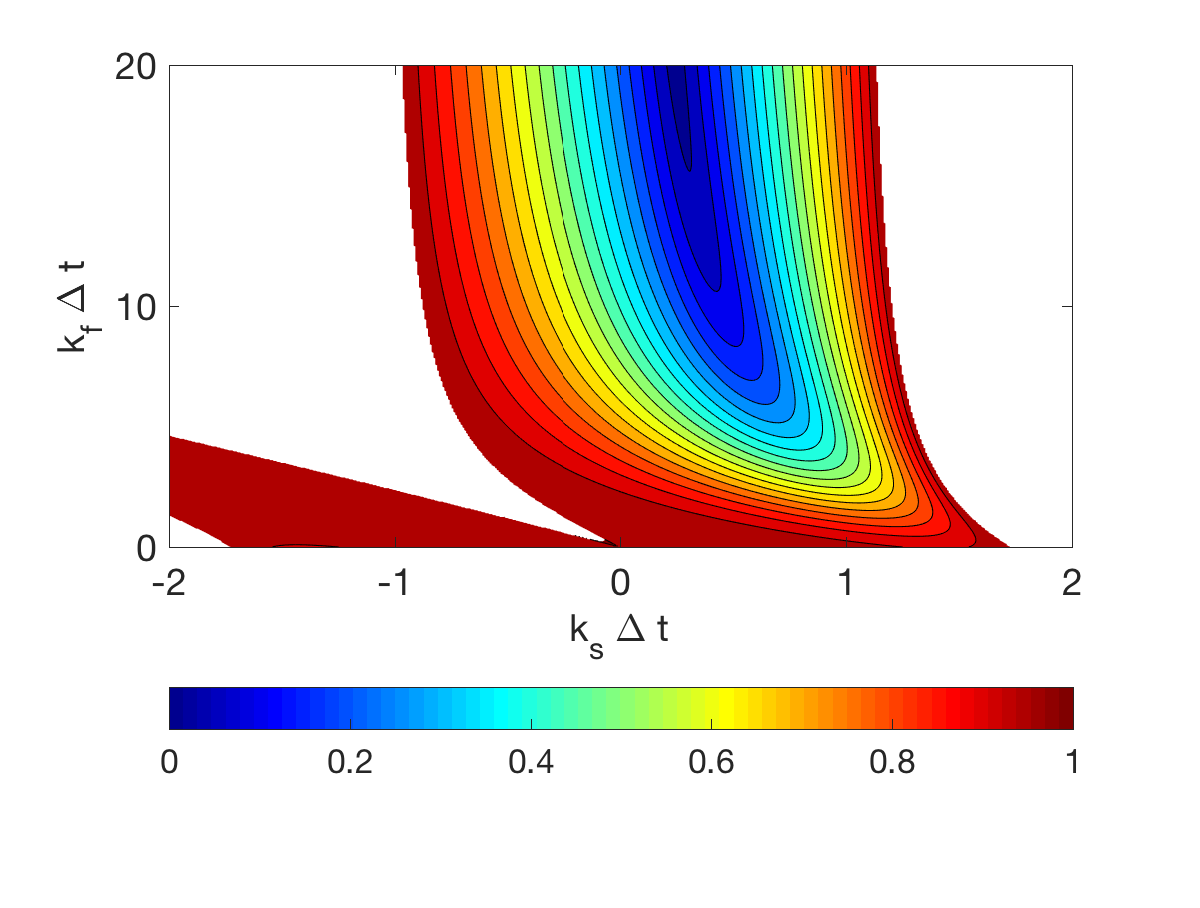
\includegraphics[width=1.5in]{figures/ARKA232_IMEX_Stability_ks=02_kf=20.eps}}
\subfigure[ARKB(2,3,2)]{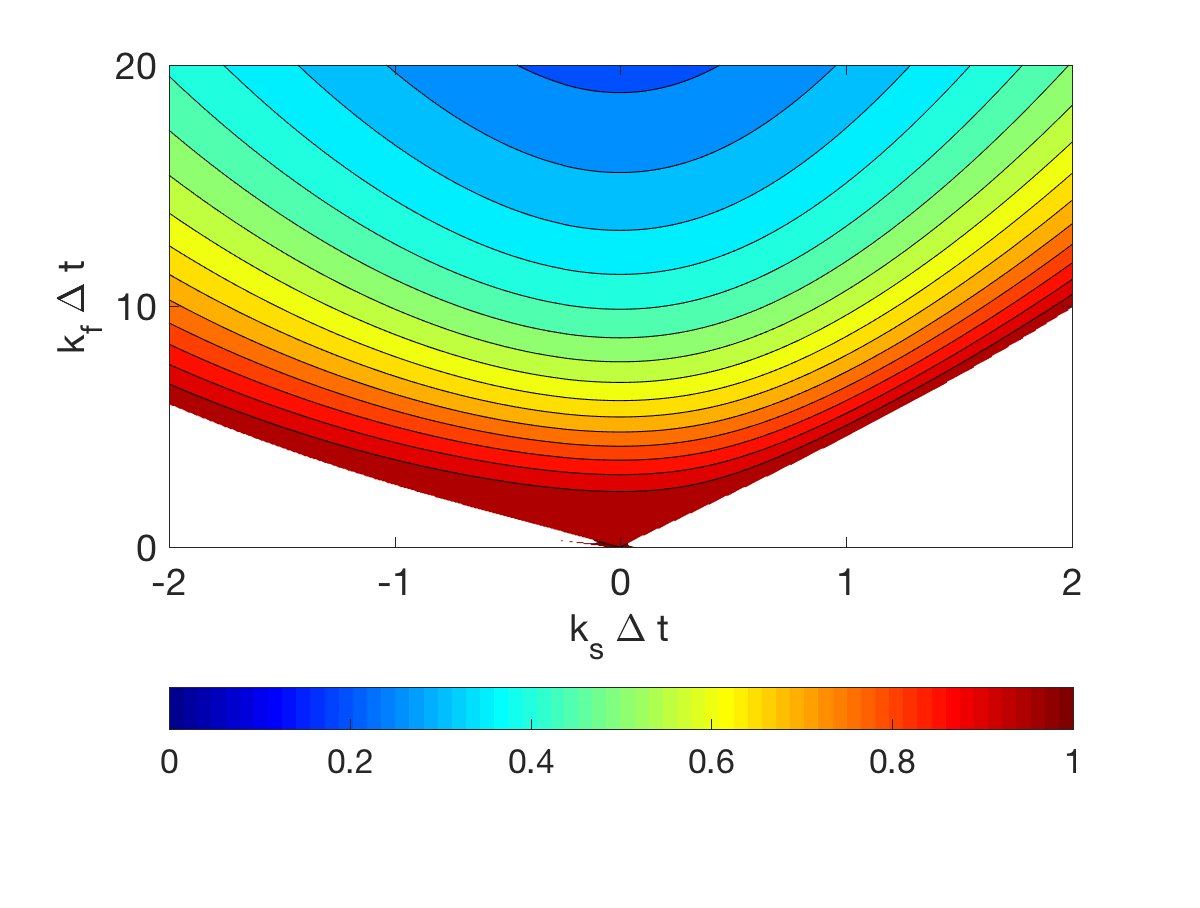
\includegraphics[width=1.5in]{figures/ARKB232_IMEX_Stability_ks=02_kf=20.eps}}
\subfigure[ARK(1,2,1)]{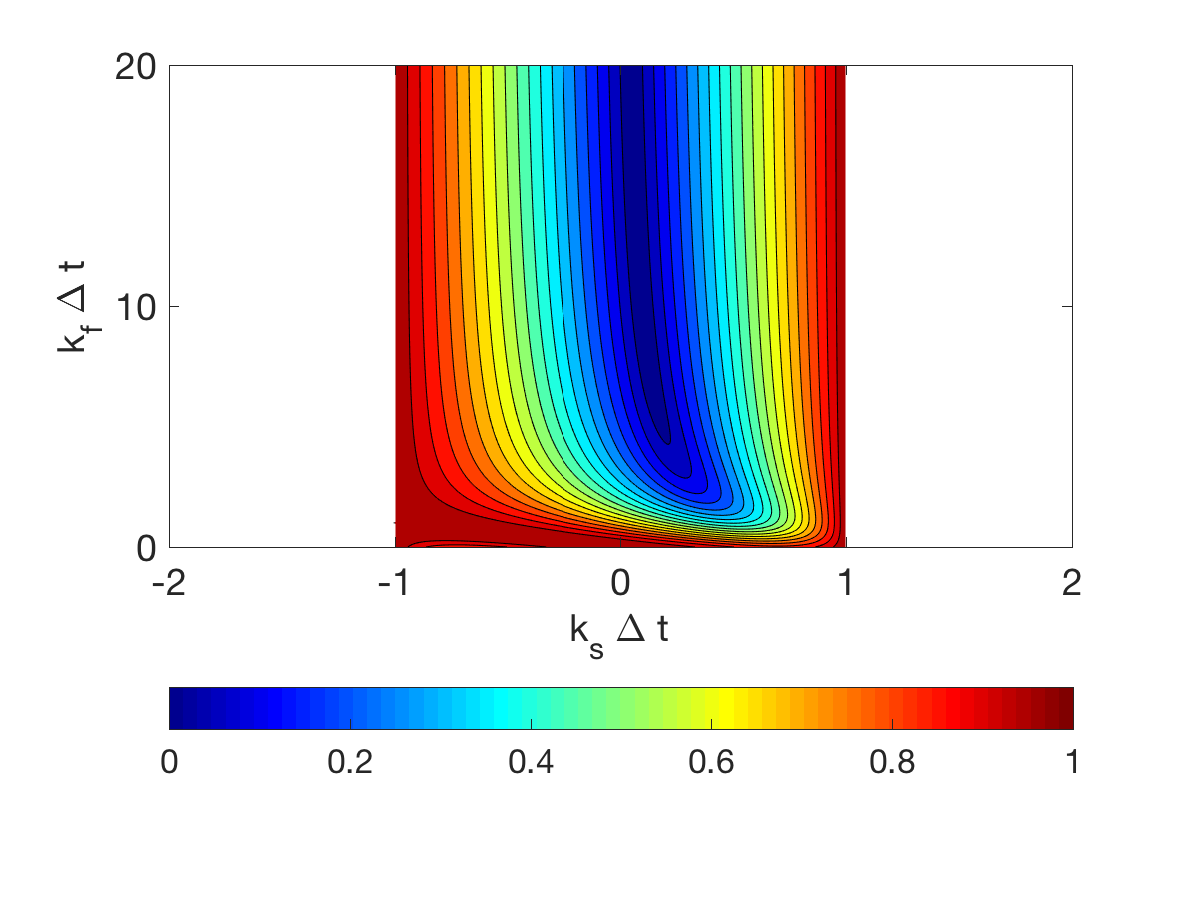
\includegraphics[width=1.5in]{figures/ARK121_Stability_ks=02_kf=20.eps}}
\end{center}
\caption{Stability regions for ARKA(2,3,2), ARKB(2,3,2), and ARK(1,2,1) for $k_s \in [-2,2]$ and $k_f \in [0,20]$.}
\label{fig:time_integration/imex_stability}
\end{figure}
Note that ARKB(2,3,2) has the typical wedge-shape stability region where the explicit part of the stability region (horizontal axis) allows larger wave speeds for the slow component than expected as we handle larger wave speeds for the fast component (vertical axis).  However, this occurs because the waves are damped (e.g., blue region). In contrast, the ARKA(2,3,2) and ARK(1,2,1) methods are attractive because at the stability limit of the method (red region) we are able to get a solution that is not damped but at the cost of adhering to smaller wave speeds for the explicit (slow) component ($\lvert k_s \lvert < 2$); the advantage of ARKA(2,3,2) over ARK(1,2,1) is that the method is second order for nonlinear terms and third order for linear terms.
\begin{table}[htbp]
\caption{Butcher tableau for a second-order IMEX Runge-Kutta ARK(2,3,2) method.}
\centering
\begin{tabular}{c|cccc}
\ST 0 & 0 & & \\
 \ST $2 - \sqrt{2}$ & $2-\sqrt{2}$ & 0 &  \\
 \ST $1$ & $1- a_{32}$  &  $a_{32}$ &  $0$  \\
 \hline
\ST  & $\frac{1}{2\sqrt{2}}$ &  $\frac{1}{2\sqrt{2}}$ & $1 - \frac{1}{\sqrt{2}}$ \\
\end{tabular}
\hspace{0.25in}
\begin{tabular}{c|cccc}
\ST 0 & 0 & & \\
 \ST $2 - \sqrt{2}$ & $1-\frac{1}{\sqrt{2}}$ & $1-\frac{1}{\sqrt{2}}$ &  \\
 \ST $1$ & $\frac{1}{2\sqrt{2}}$  &  $\frac{1}{2\sqrt{2}}$ &  $1 - \frac{1}{\sqrt{2}}$  \\
 \hline
\ST  & $\frac{1}{2\sqrt{2}}$ &  $\frac{1}{2\sqrt{2}}$ & $1 - \frac{1}{\sqrt{2}}$ \\
\end{tabular}
\label{table:time_integration/imex/ark232}
\end{table}
\begin{table}[ht]
\caption{Butcher tableau for a first-order IMEX Runge-Kutta ARK(1,2,1) method.}
\centering
\begin{tabular}{c|cccc}
\ST 0 && 0 && \\
 \ST $1$ && $1$ && 0  \\
 \hline
\ST  && 0 &&  $1$ \\
\end{tabular}
\hspace{0.5in}
\begin{tabular}{c|cccc}
\ST 0 &&  0 &&  \\
 \ST $1$ && 0 && $1$  \\
 \hline
\ST  && 0 &&  $1$ \\
\end{tabular}
\label{table:time_integration/imex/ark121}
\end{table}

\subsection{Nonlinear vertical implicit treatment}
The aforementioned linear implicit and nonlinear explicit decomposition for the time stepping has been extended to nonlinear vertical implicit and nonlinear explicit decomposition. The nonlinear implicit treatment is aimed to eliminate the stiffness and the CFL constraint in the vertical direction, and is restricted to the single column configuration. Therefore, each single column can be implicitly solved independently. 

Let us rewrite Eq.~\eqref{eq:IMEX} as
\begin{equation}
\label{eq:IMEX_v3}
\frac{\partial\vec{Y}}{\partial t} =  \Tvector_I(\vec{Y}) + \Tvector_{d'}(\vec{Y})
\end{equation}
where $\Tvector_I(\vec{Y})$ represents the vertical implicit tendencies, and $\Tvector_{d'}$ captures the nonlinear remainder tendencies after the nonlinear implicit tendencies are taken into account.  

If for now we neglect $\Tvector_{+f}$ (e.g., view it as included in  $\Tvector_{d'}$), a first 3D-IMEX algorithm with superstepping of the slow tendencies takes the following form:
\begin{algorithm}
\label{alg:3d-imex_nonlinear_imp}
\begin{algorithmic}
\State
\Function{3D-IMEX with Nonlinear Vertical Implicit and Explicit Decomposition}{}
\For{$i=1:S$} 
\State $ \vec{Y}^{(i)} - \Delta t \widetilde{a}_{ii} \Tvector_I(\vec{Y}^{(i)})=\vec{Y}^{n} + \Delta t \sum_{j=1}^{i-1} \left( a_{ij} \Tvector_{d'}(\vec{Y}^{(j)}) 
+ \widetilde{a}_{ij} \Tvector_I( \vec{Y}^{(j)} )\right)$ 
\EndFor %i
\State $\vec{Y}^{n+1}=\vec{Y}^{n} + \Delta t \sum_{i=1}^{S} b_{i} \left[ \Tvector_{d'}(\vec{Y}^{(i)}) 
+ \Tvector_I(\vec{Y}^{(i)}) \right]$
\EndFunction
\end{algorithmic}
\end{algorithm}

In Alg.\ \ref{alg:3d-imex_nonlinear_imp}, the nonlinear update equation can be written as 
\begin{equation}
\label{eq:newton-v1}
\vec{F}(\vec{Y}) = \vec{F}^{rhs}
\end{equation}
here $\vec{F}(\vec{Y})= \vec{Y} - \Delta t \widetilde{a}_{ii} \Tvector_I(\vec{Y})$  and $\vec{F}^{rhs} = \vec{Y}^{n} + \Delta t \sum_{j=1}^{i-1} \left( a_{ij} \Tvector_{d'}(\vec{Y}^{(j)}) 
+ \widetilde{a}_{ij} \Tvector_I( \vec{Y}^{(j)} )\right)$, and solved by Newton's method. Newton's method iteratively solve $\vec{Y}$ by 
\begin{equation}
    \vec{Y}^{n+1} = \vec{Y}^{n} - \vec{J}(\vec{Y}^{n})^{-1}\cdot [\vec{F}(\vec{Y}^n) - \vec{F}^{rhs}]\textrm{ and }  \vec{J}(\vec{Y}) = \frac{d\vec{F}}{d\vec{Y}}(\vec{Y})
\end{equation}
%
To avoid the computing of the Jacobian matrix $\vec{J}$, the Newton's increment $\Delta\vec{Y}$
\begin{equation} 
\vec{J}(\vec{Y}^{n})\Delta\vec{Y} = \vec{F}(\vec{Y}^n) -\vec{F}^{rhs}
\end{equation}
 is computed by the batched Generalized Minimal Residual method. The batched parallelization is attributed to the single column configuration. And the Jacobian action is approximated by the finite difference method, as follows,  
 \begin{equation}
     \vec{J}(\vec{Y}^{n})\Delta \vec{Y} \approx \frac{\vec{F}(\vec{Y}^n + \epsilon \Delta \vec{Y}) - \vec{F}(\vec{Y}^n)}{\epsilon}
 \end{equation}
 
 To accelerate the Generalized Minimal Residual method, preconditioner $\vec{P} \approx \vec{J}$ is introduced. Instead of solving for $\Delta \vec{Y}$, we solve  $\widetilde{\Delta \vec{Y}}$, as follows, 
\begin{equation*}
    \vec{J}(\vec{Y}^{n}) \vec{P}^{-1} \widetilde{\Delta \vec{Y}} = \vec{F}(\vec{Y}^n) \textrm{ and } \vec{P}^{-1}\Delta \vec{Y} = \widetilde{\Delta \vec{Y}}
\end{equation*}
    
The matrix $\vec{P}$ is approximated by the finite difference method 
\begin{equation*}
 \vec{P}[:, i] \approx \frac{\vec{F}(\vec{Y}^n + \epsilon e_i) - \vec{F}(\vec{Y}^n)}{\epsilon}
\end{equation*}
here $e_i = [0,...,0,1,0,...0]$ and $\vec{P}[:, i]$ is the i-th column of $\vec{P}$. The number of column is the degrees of freedom of each column. It is expensive to build the preconditioner matrix, but we can update it every $n$ iterations. Moreover, to leverage the banded structure of the Jacobian matrix $\vec{J}$, we can use $e_{i_1, i_2, ...i_k} =[...,1,0,...,0,1, ...]$, and construct $\vec{P}[:,i_1]$,  $\vec{P}[:,i_2]$, ... ,$\vec{P}[:,i_k]$ at once. Therefore, the number of implicit function calls reduces from the degrees of freedom of each column $O(N)$ to the band width of the matrix, $O(1)$. 
    






\clearpage
\section{Fully Explicit Multirate Method: Substepping}
\label{sec:substepping}

\subsection{Split-Explicit as in Wicker-Skamarock}
To discretize the equations in time using a simple partitioned Runge-Kutta method (as in Wicker-Skamarock MWR 2002), let us describe the method using the following 3-partition system of ordinary differential equations:
\[
\diff{\vec{Y}}{t}= L_I(\vec{Y}) + \Tvector_{d'} + \Tvector_{-s}
\]
where $\Tvector_{d'}=\Tvector^N_{I}(\vec{Y}) + \Tvector_{d}$, and the right-hand side is ordered in ascending wave-speed order, i.e., 
the wave speed $\mathcal{S}$ of the different components are ordered as follows $\mathcal{S}(L_I) > \mathcal{S}(\Tvector_{d'})$, etc.

The algorithm describing the 3-partition multirate RK method is highlighted in Alg.\ \ref{alg:split-explicit-WS2002}.
\comment{
\begin{algorithm}
\label{alg:4-prk}
\begin{algorithmic}
\State
\Function{4-Partition Multirate RK}{}
\State update $\Tvector_{-s}(\magenta{ \vec{Y}^{n-s}})$
\State $\vec{Y}^{(i)}=\vec{Y}^n$ 
\For{$i=1:I$} 
\State $\vec{Y}^{(j)}=\vec{Y}^{(i)}$ \Comment update $\Tvector_{d'}(\red{ \vec{Y}^{(i)} })$
\For{$j=1:J$} 
\State $\vec{Y}^{(k)}=\vec{Y}^{(j)}$ \Comment update $\Tvector_{+f}(\blue{ \vec{Y}^{(j)} })$
\For{$k=1:K$} 
\State $\vec{Y}^{(k)}=\vec{Y}^{(j)} + \Delta \tau \left[ \Tvector_{-s}(\magenta{ \vec{Y}^{n-s} }) + \Tvector_{d'}(\red{ \vec{Y}^{(i)}}) + \Tvector_{+f}(\blue{ \vec{Y}^{(j)} }) + L_I(\vec{Y}^{(k)}) \right]$
\EndFor %k
\State $\vec{Y}^{(j)}=\vec{Y}^{(k)}$
\EndFor %j
\State $\vec{Y}^{(i)}=\vec{Y}^{(j)}$
\EndFor %i
\State $\vec{Y}^{n+1}=\vec{Y}^{(i)}$
\EndFunction
\end{algorithmic}
\end{algorithm}
}
\begin{algorithm}
\label{alg:split-explicit-WS2002}
\begin{algorithmic}
\State
\Function{3-Partition Split-Explicit General RK}{}
\State update $\Tvector_{-s}(\magenta{ \vec{Y}^{n-s}})$
\State $\vec{Y}^{(i)}=\vec{Y}^n$ 
\For{$i=2:I+1$} 
\State update $\Tvector_{d'}(\red{ \vec{Y}^{(i)} })$
\State $\vec{Y}^{(m)}=\vec{Y}^{n}$ 
\For{$m=1:c_i \cdot M$} 
\State $\vec{Y}^{(m)}=\vec{Y}^{(m)} + \frac{\Delta t}{M} \left[ \Tvector_{-s}(\magenta{ \vec{Y}^{n-s} }) + \Tvector_{d'}(\red{ \vec{Y}^{(i)}}) + L_I(\vec{Y}^{(m)}) \right]$
\EndFor %k
\State $\vec{Y}^{(i)}=\vec{Y}^{(m)}$
\EndFor %i
\State $\vec{Y}^{n+1}=\vec{Y}^{(i)}$
\EndFunction
\end{algorithmic}
\end{algorithm}
In Alg.\ \ref{alg:split-explicit-WS2002} the red and magenta fonts indicate terms that are frozen within the $m$-loop and is what allows a performance gain since these terms are not computed within this loop. Also, 
the RK coefficients are written in low-storage form as follows $a_{i+1}=\frac{1}{I-i+1}$ with $c_i=a_i$. Unfortunately, this approach only yields a convergence rate of 1 since the inner loop uses forward Euler.

\comment{
If all partitions are of the same order then the effective time-step of each partition is 
\[
\mathcal{O} \left( \frac{\Delta t}{N_{RK}^{p-1}} \right)
\]where $N_{RK}$ is the order of the RK method and $p$ refers to the partition (e.g., for $p=1$ the time-step is $\Delta t$, for $p=2$ the time-step is $\Delta t/N_{RK}$, and for $p=3$ the time-step is $\Delta t/N_{RK}^2$). 

If the embedded partition described in Alg.\ \ref{alg:4-prk} yields an insufficiently small time-step to maintain stability of the fastest waves then substepping can be added as shown in Alg.\ \ref{alg:4-prk_v2} where an additional loop ($m$-loop) is inserted before the $k$-loop.
\begin{algorithm}
\label{alg:4-prk_v2}
\begin{algorithmic}
\State
\Function{4-Partition Multirate RK with Euler Substepping}{}
\State update $\Tvector_{-s}(\magenta{ \vec{Y}^{n-s}})$
\State $\vec{Y}^{(i)}=\vec{Y}^n$ 
\For{$i=1:I$} 
\State $\vec{Y}^{(j)}=\vec{Y}^{(i)}$ \Comment update $\Tvector_{d'}(\red{ \vec{Y}^{(i)} })$
\For{$j=1:J$} 
\State $\vec{Y}^{(m)}=\vec{Y}^{(j)}$ \Comment update $\Tvector_{+f}(\blue{ \vec{Y}^{(j)} })$
\For{$m=1:M$} 
\State $\vec{Y}^{(k)}=\vec{Y}^{(m)}$
\For{$k=1:K$} 
\State $\vec{Y}^{(k)}=\vec{Y}^{(m)} + \Delta \tau \left[ \Tvector_{-s}(\magenta{ \vec{Y}^{n-s} }) + \Tvector_{d'}(\red{ \vec{Y}^{(i)}}) + \Tvector_{+f}(\blue{ \vec{Y}^{(j)} }) + L_I(\vec{Y}^{(k)}) \right]$
\EndFor %k
\State $\vec{Y}^{(m)}=\vec{Y}^{(k)}$
\EndFor %m
\State $\vec{Y}^{(j)}=\vec{Y}^{(m)}$
\EndFor %j
\State $\vec{Y}^{(i)}=\vec{Y}^{(j)}$
\EndFor %i
\State $\vec{Y}^{n+1}=\vec{Y}^{(i)}$
\EndFunction
\end{algorithmic}
\end{algorithm}
In Alg.\ \ref{alg:4-prk_v2}
$\Delta \tau=\frac{\Delta t}{M} a_i^I a_j^J a_k^K$.
}

\subsection{Multirate as in Wensch-Knoth}
The approach presented previously has been used in various nonhydrostatic codes and has been shown to work effectively to increase the time-to-solution of the problem.  However, the Butcher tableaux required in that approach is rather limited (only one type of RK method was originally proposed and forward Euler was used in the inner/fast loop which is not ideal for high-order spatial discretization methods).  A general approach was introduced by Wensch and Knoth in order to give split-explicit methods a more formal mathematical formulation.  Wensch and Knoth generalized this approach further to yield multirate methods that have better than 1st order convergence rates which we now describe in Alg.\ \ref{alg:general_explicit_multirate} for the following three-partitioned equation
\[
\diff{\vec{Y}}{t}= L_I(\vec{Y}) +  \Tvector_{d'} + \Tvector_{-s}.
\]
\begin{algorithm}
\label{alg:general_explicit_multirate}
\begin{algorithmic}
\State
\Function{3-Partition General Explicit Multirate RK}{}
\State $\vec{Q}^{(1)}=\vec{Y}^n$ 
\For{$i=2:I+1$} 
\State $\red{r_i}=\Tvector_{-s}(\magenta{ \vec{Y}^{n-s}}) + \sum_{j=1}^{i-1} \widetilde{a}_{i,j} \Tvector_{d'}(\red{\vec{Q}^{(1)}})$
\State $\vec{V}_{i,1}=\vec{Q}^{(i-1)}$
\For{$j=2:J+1$} 
\State $\vec{V}_{i,j}=\vec{V}_{i,j-1} + \Delta t \sum_{k=1}^{j-1} \widetilde{a}_{j,k} \left[ \red{r_i} + \widetilde{c}_{i} L_I(\vec{V}_{i,k}) \right]$ 
\EndFor %j
\State $\vec{Q}^{(i)}=\vec{V}_{i,J+1}$
\EndFor %i
\State $\vec{Y}^{n+1}=\vec{Q}^{(I+1)}$
\EndFunction
\end{algorithmic}
\end{algorithm}
where 
\[
\widetilde{a}_{i,j}=\left\{
\begin{array}{cc}
  {a}_{i,j}-{a}_{i-1,j}   &  i < s+1 \\
  {b}_{j}-{a}_{s,j}   &  i = s+1  
\end{array}
\right.
\]
and
\[
\widetilde{c}_{i}=\left\{
\begin{array}{cc}
  {c}_{i}-{c}_{i-1}   &  i < s+1 \\
  1-{c}_{s}   &  i = s+1  
\end{array}
\right.
\]
with $a$, $b$, and $c$ being the Butcher tableau coefficients found in Eq.\ \eqref{eq:butcher_tableau} and $s$ denotes the number of stages.  The only constraint on this algorithm is that the coefficients $c$ increase monotonically. If they do not, we can still use this approach but Alg.\ \ref{alg:general_explicit_multirate} would have to be modified.  Using this approach, the order of the scheme is min(order(I),order(J)) where  order(I) and order(J) are the orders of the RK methods with respect to the $I$ and $J$ loops.

\subsection{Multirate as in Wensch-Knoth for Low-Storage Methods}
Algorithm \ref{alg:general_explicit_multirate} represents a general multirate time-integration form that can be used with any comnbination of methods provided that they are written in Butcher tableau form.  However, the Butcher form requires the storage of stage values which may not be ideal on GPUs. Instead, we now rewrite this algorithm for low-storage RK methods which we describe below.
\begin{algorithm}
\label{alg:general_explicit_multirate/lsrk}
\begin{algorithmic}
\State
\Function{3-Partition General Explicit Multirate LSRK}{}
\State $\vec{y}=\vec{Y}^n$ 
\For{$i=1:I$} 
\State $\red{r_{slow}}=\Tvector_{-s}(\magenta{ \vec{Y}^{n-s}}) + A_i r_{slow} + \Tvector_{d'}(\red{\vec{y}})$
\State $\widetilde{c}_i=c_i - c_{i-1}$
\For{$j=1:J$} 
\State $r_{fast}=A_j r_{fast} + L_I(\vec{y}) + \frac{B_i}{c_i - c_{i-1}} \red{r_{slow}}$ 
\State $\vec{y} = \vec{y} + \Delta t \widetilde{c}_i  B_j r_{fast}$
\EndFor %j
\EndFor %i
\EndFunction
\end{algorithmic}
\end{algorithm}
The multirate LSRK presented in Alg.\  \ref{alg:general_explicit_multirate/lsrk} is the method currently implemented in CLIMA where the 5-stage (Kennedy-Carpenter) and 14-stage (Niegemann et al.) LSRK methods are included, where the coefficients $A$ and $B$ are the typical coefficients in Williamson low-storage form.

\section{Stability of Explicit Methods in CLIMA}
Figure \ref{fig:time_integration/explicit_stability} shows the explicit stability region of some of the time-integrators available in CLIMA; for comparison, the classical RK4 is included.  Figure \ref{fig:time_integration/explicit_stability}(a) shows the stability region per-stage whereas \ref{fig:time_integration/explicit_stability}(b) shows the total stability region.  In these figures, the vertical axis represents the stability for thd non-dissipative components (e.g., 1st order hyperbolic operators) whereas the horizontal axis the dissipative components (e.g., second order elliptic operators and the dissipation introduced by the Rusanov numerical flux).  Although we cannot use these figures to predict the exact Courant numbers for each of the methods, we can use these figures to get a sense of the difference in the stability regions for each of the time-integrators. For example, we can see that the explicit tableau for the IMEX ARK(2,3,2) method is much smaller than that for the LSRK(14,4) method. In fact, Fig.\ \ref{fig:time_integration/explicit_stability}(b) shows that the LSRK(14,4) method has a particularly large stability region (compared to the other methods) for the dissipative components.
\begin{figure}[htbp]
\begin{center}
\subfigure[Per-stage Stability]{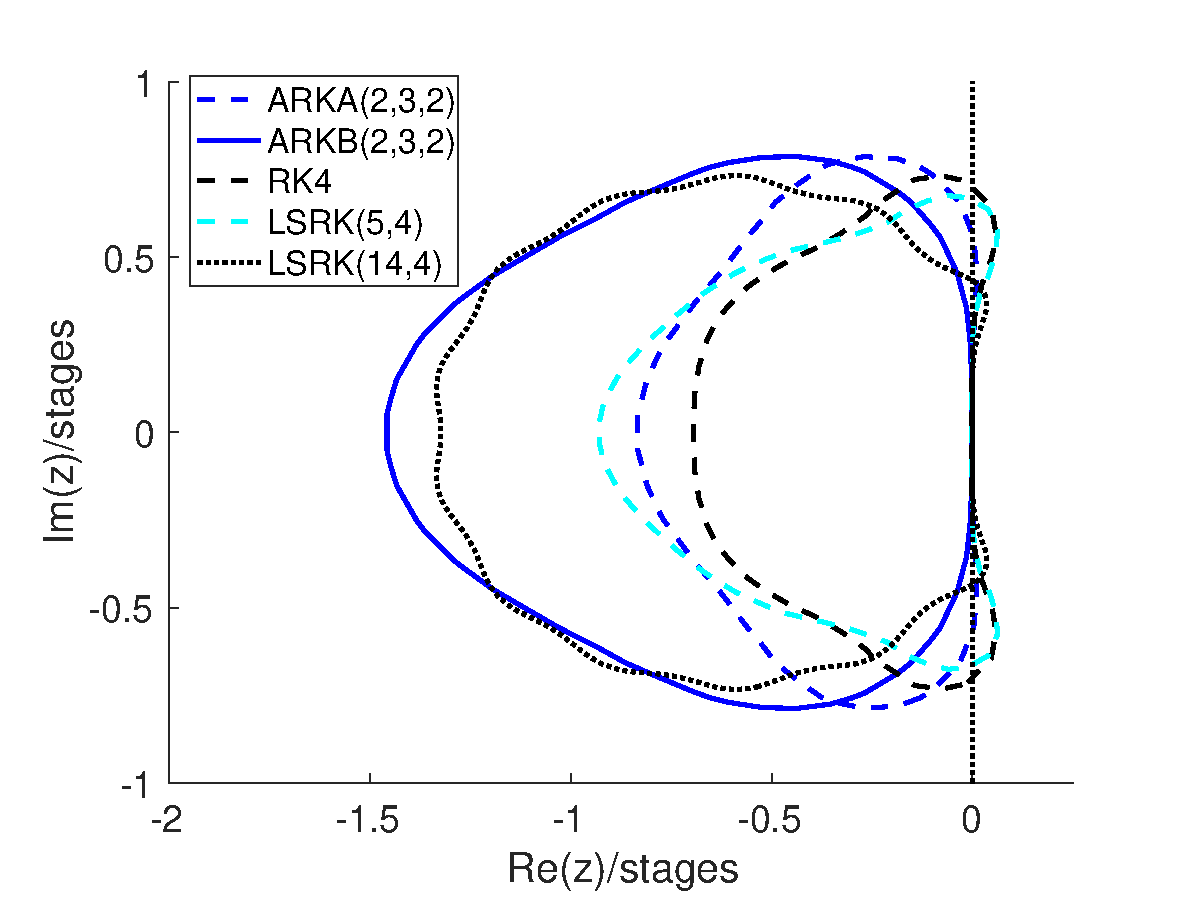
\includegraphics[width=2.25in]{figures/Stability_CLIMA_RK_Methods_Per_stage_Stability.eps}}
\subfigure[Total Stability]{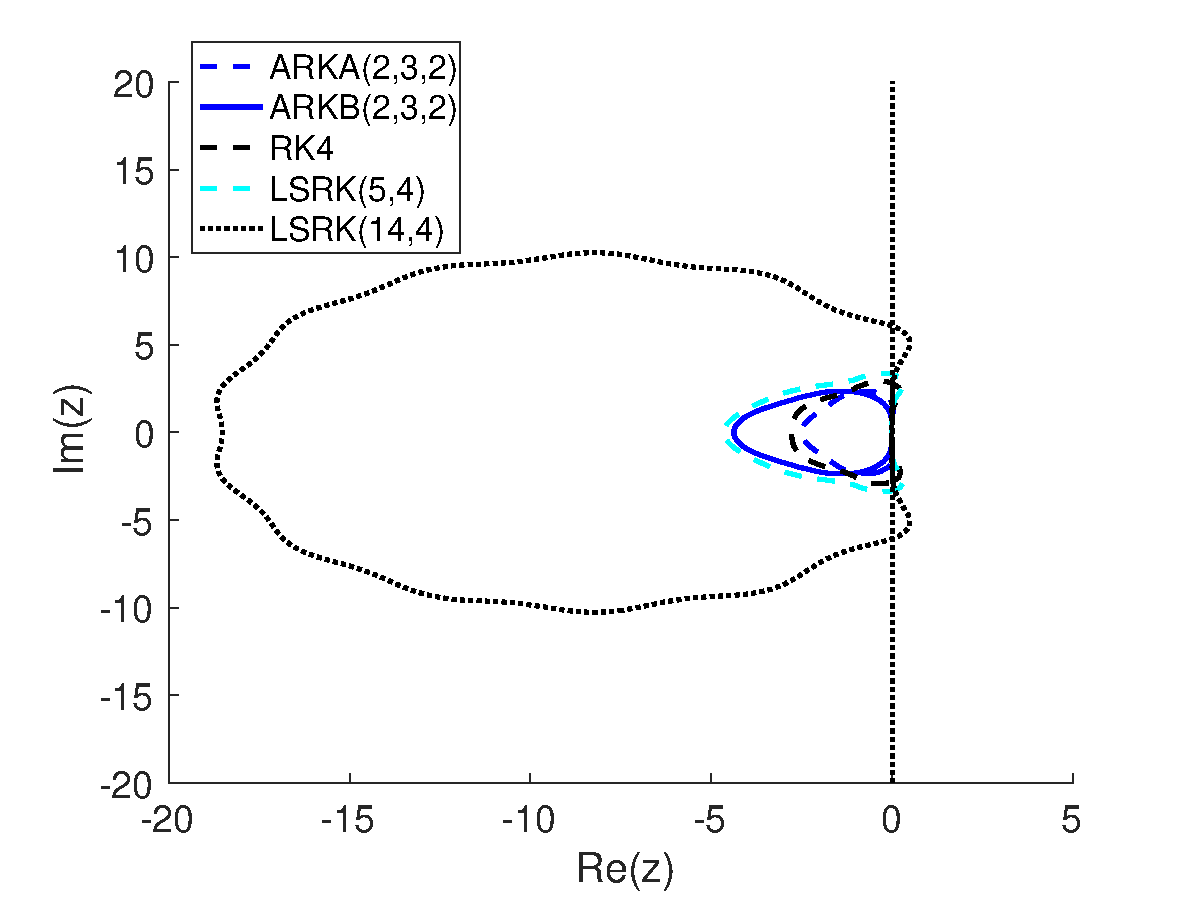
\includegraphics[width=2.25in]{figures/Stability_CLIMA_RK_Methods_Total_Stability.eps}}
\end{center}
\caption{Explicit stability regions for the some time-integrators in CLIMA. Panel (a) shows the stability region per stage while panel (b) shows the total stability region.
\hlc[green]{Toby: I think one section we need here and that would be useful generally is would contain rules of thumb for the best stable Courant number based on horizontal spacing for each time stepping method used in the ClIMA code. Example: Currently, as default, we use a 1D-IMEX with the ARK2GKC time stepper and a courant number of 0.4. One can see this in the CLIMA master branch src/Driver/Driver.jl l.210 and src/Driver/Configurations.jl l.31. I think having this in the design doc and matching the codebase would be fantastic}
}
\fxg{Thomas is working on this}
\label{fig:time_integration/explicit_stability}
\end{figure}

\section{Guidelines for Selecting the Time-Step}
The time-step restriction for an explicit method must satisfy the stable Courant number for the specific time-integrator and must be selected from the following constraints
\[
\Delta t_{\mathrm{explicit}} = min \left( \frac{C \Delta s_i}{u_i + a}, \frac{C \Delta s_i^2}{\nu} \right)
\]
where $C$ is the stable Courant number, $u_i$ denotes the velocity components, $a$ the speed of sound, $\Delta s_i$ the grid spacing along the direction ($x_1,x_2,x_3$), and $\nu$ the kinematic viscosity. The first term on the right is the time-step condition due to the non-dissipative components while the second term to the dissipation. For explicit time-integrators, we have to find the minimum time-step that satisfies this condition along all three spatial directions.

In the case of 3D-IMEX, the largest stable time-step is obtained from the conditions
\[
\Delta t_{\mathrm{3D-IMEX}} = min \left( \frac{C \Delta s_i}{u_i}, \frac{C \Delta s_i^2}{\nu} \right)
\]
where we now are unconditionally stable with respect to the speed of sound (since these terms are solved implicitly) and where we assume here that the diffusion is handled fully explicitly.

In the case of 1D-IMEX along the vertical direction, the largest stable time-step is obtained from the conditions
\[
\Delta t_{\mathrm{1D-IMEX}} = min \left( \frac{C \Delta s_H}{u_H+a}, \frac{C \Delta s_V}{u_V}, \frac{C \Delta s^2}{\nu} \right)
\]
where the subscripts $H$ and $V$ denote the \emph{horizontal} and \emph{vertical} components. Again,here we assume that the viscosity is handled fully explicitly.

\hl{Akshay: We currently have MultirateRungeKutta.jl which allows a model to be split into its fast / slow components (we have the isentropic vortex example demonstrating use of this, and I have an example with the Rayleigh-Benard case with two explicit rates, and an LES example with IMEX + 1 horizontal rate: (a)does the current setup allow us to use more than 2 rates in the horizontal (if so, where in the source code should I be looking? (We'd like to move towards vertical implicit solve + 2 horizontal explicit rates) (b)The explicit solver type supported by MultirateRungeKutta is restricted to the LSRK2N type; is this the recommended solver in the default case given the stability margins? (c)The CFL calculator would help in setting up a general method for multirate timestepping. (see solver setup() in Driver.jl))?}
\fxg{Akshay, let me check on this for you.}

\chapter{temporary CG write up}

Inlcude a snappy intro here

\section{Discrete spaces for CG}
All calculations for Spectral Elements methods are done on a reference element, in our case, we consider the reference cube $[-1,1]^3$. Now let $\overrightarrow{x} = (x_1,x_2,x_3)$ be the coordinate vector defining the position of a point on the reference cube in Cartesian coordinates. Next, we take $\overrightarrow{r} = (r_1,r_2,r_3)$ to be the position vector of a point in the computation domain taken in possibly curvilinear coordinates. We note the computation domain as $\Omega$ and the space of polynomials up to a degree d and defined on the reference cube $[-1,1]^3$ as follows:
\begin{equation}
    P_d :=span_{i,j,k=0}^d(x_1)^i(x_2)^j(x_3)^k,
\end{equation}
we can then define the cardinal functions $\phi_{\overrightarrow{l}} = \prod_{\alpha=1}^3 \varphi_{i^{\alpha}}(x^{\alpha})$ for $i^{\alpha}=0,..,d$ and $\overrightarrow{l} \in \{0,..,d\}^3$. The cardinal functions interpolate the 3D Legendre-Gauss-Lobatto (LGL) points of degree d $\overrightarrow{\xi_{\overrightarrow{l}}}:=\sum_{\alpha}\xi_{i^{\alpha}}e_{\alpha}$, where $e_{\alpha},\alpha = 1,2,3$ are the Cartesian unit vectors on the reference cube.  Thus for a function g, we can obtain the following the expansion using the cardinal functions:
\begin{equation}
    g(\overrightarrow{x}) = \sum_{\overrightarrow{l}}g(\overrightarrow{\xi_{\overrightarrow{l}}})\phi_{\overrightarrow{l}}(\overrightarrow{x}) = \textbf{g}^T\boldsymbol{\phi}(\overrightarrow{x}),
\end{equation}

where $\mathbf{g}$ is defined as $\mathbf{g}=\sum_{\overrightarrow{l}}g(\overrightarrow{\xi_{\overrightarrow{l}}})e_{i^1} \otimes e_{i^2} \otimes e_{i^3} \in \mathbb{R}^{(d+1)^3\times 1}$ \\
And \begin{equation}
    
\boldsymbol{\phi}=\sum_{\overrightarrow{l}}\phi_{\overrightarrow{l}}(\overrightarrow{x})e_{i^1} \otimes e_{i^2} \otimes e_{i^3} \in \R^{(d+1)^3\times 1}.
\end{equation}

Here $()^T$ represents the matrix transpose operator, $e_i \in \{0,1\}^{(d+1)\times 1}$ is column (i+1) of the square identity matrix of size (d+1). $\otimes$ denotes the kroenecker product. Keeping all of this in mind we can now proceed to split the domain up into a  conforming mesh of M hexahedral elements denoted $\Omega_m$, where $m \in \{1,..,M\}$. We assume that for each element there exists a $C^1$ map from it to the reference cube. This allows us to define this map and its inverse as follows:
\begin{equation}
    \overrightarrow{r}=\overrightarrow{r}(\overrightarrow{x},m), \hspace{10pt} \overrightarrow{x}=\overrightarrow{x}(\overrightarrow{r},m),
\end{equation}

since elements share boundaries, these mappings need to agree along the boundaries of neighboring elements. This means that for $A = \Omega_m \cap \Omega_n$, $\overrightarrow{r}=\overrightarrow{r}(\overrightarrow{x},m) \vert_A  = \overrightarrow{r}=\overrightarrow{r}(\overrightarrow{x},n) \vert_A$. This gives us that the tangential derivatives of $\overrightarrow{r}$ also agree along A since these derivatives are done along the boundary. The normal derivatives on the other hand are allowed to not agree since the mapping do not necessarily coincide within the interiors of neighboring elements.

Next, we define the piecewise-polynomial spectral element spaces $\mathbf{V}^0$ and $\mathbf{V}^1$
\begin{equation}
    \mathbf{V}^0 = \{f\in(\mathbf{L}^2\Omega):f(\overrightarrow{r}(.,m))\in P_d, \forall m\} = span_{m=1}^M\{\phi_{\overrightarrow{l}}}(\overrightarrow{x}(.,m))\}_{\overrightarrow{l}},
\end{equation}
\begin{equation}
    \mathbf{V}^1 = C^0(\Omega)\cap \mathbf{V}^0.
\end{equation}

Functions belonging to $\mathbf{V}^0$ are polynomials within a given element but are allowed to be discontinuous across element boundaries. For a continuous Galerkin formulation, the global solution can only depend on functions in $\mathbf{V}^1$, the subspace of continuous function within $\mathbf{V}^0$. However the less restrictive space $\mathbf{V}^0$ is still useful for many intermediate quantities before reaching the global solution. Next we take the following quantities $M_d = dim(\mathbf{V}^0) = (d+1)^3M$ and $L = dim(\mathbf{V}^1) < M_d$. By piecing together the right combination of $M_d$ local basis functions $\phi_{\overrightarrow{l}}(\overrightarrow{x}(\overrightarrow{r},m))$ we can obtain the global basis functions $\{\Phi_k\}(\overrightarrow{r})\}_{k=1}^L \in \mathbf{V}^1$. We now define the L interpolation points for these global basis functions as follows:
\begin{equation}
    \{\overrightarrow{r}_{\overrightarrow{k}}\}_{k=1}^L:= \cup_{m=1}^M \overrightarrow{r}(\{\overrightarrow{\xi}_{\overrightarrow{l}}\}_{\overrightarrow{l}\in\{0,...,d\}^3},m).
\end{equation}
This means $\Phi_{k^{'}}(\overrightarrow{r}_k) = \delta_{k^{'} k}$. We next note that for every global interpolation point in the physical domain $\overrightarrow{r}_{k}$, there must exist at least one element $\Omega_m$ such that there is at least one LGL node that verifies $\overrightarrow{\xi}_{\overrightarrow{l}}=\overrightarrow{x}(\overrightarrow{r}_k,m)$. For a 3D domain $\Omega$ this is verified for exactly one element $\Omega_m$, if $\overrightarrow{r}_k$ is either an element interior node or a global boundary node. On the other hand, if $\overrightarrow{r}_k$ belongs exactly to two elements than it is an element-face-interior node. Finally, if it belongs to more than two elements than it is an edge-interior or vertex node.
Analogously to scalars, we define the following spaces for vectors on $\Omega$:
\begin{equation}
\mathbf{V}_{con}^0 = \{\overrightarrow{u}\in(\mathbf{L}^2\Omega)^3:u^{\alpha}\in \mathbf{V}^0, \alpha=1,2,3\}
\end{equation}
\begin{equation}
    \mathbf{V}_{con}^1 = C^0(\Omega)^3\cap \mathbf{V}_{con}^0.
\end{equation}
\begin{equation}
\mathbf{V}_{cov}^0 = \{\overrightarrow{u}\in(\mathbf{L}^2\Omega)^3:u_{\beta}\in \mathbf{V}^0, \beta=1,2,3\}
\end{equation}
\begin{equation}
    \mathbf{V}_{cov}^1 = C^0(\Omega)^3\cap \mathbf{V}_{cov}^0,
\end{equation}
where $u^{\alpha}$ and $u_{\beta}$ are respectively the contravariant and covariant components of the vector $\overrightarrow{u}$. $\forall \overrightarrow{u} \in \mathbf{V}_{cov}^1 \cup \mathbf{V}_{con}^1, \overrightarrow{u}  \in C^0(\Omega)^3$ and it's components (covariant or contravariant) are polynomials in each of the elements in the domain.
Following (3.1.2) and taking $g(\overrightarrow{x}=f(\overrightarrow{r}(\overrightarrow{x},m)$ for a function $f \in \mathbf{V}^0$ we can expand f using the cardinal function defined in (3.1.3) as follows:

\begin{equation}
    f(\overrightarrow{r})=\sum_{\overrightarrow{l}}f(\overrightarrow{r}(\overrightarrow{\xi}_{\overrightarrow{l}},m))\phi_{\overrightarrow{l}}(\overrightarrow{x}(\overrightarrow{r},m) = \mathbf{f}_m^T\boldsymbol{\phi}(\overrightarrow{x}(\overrightarrow{r},m)),
\end{equation}
where $\mathbf{f}_m$ is analogous to \mathbf{g} and we define $\mathbf{f} = (\mathbf{f}_1^T,\mathbf{f}_2^T,...,\mathbf{f}_M^T ) \in \mathbb{R}^{M_d\times1}$. The column vector $\mathbf{f}_m$ holds the values of f along each individual element $\Omega_m$ and as such also contains the multiple values taken at redundant nodes (belonging to more than 1 element), this is because $f \in \mathbf{V}^0$ and is allowed to be discontinuous along element interfaces. Since we require solutions that are in $\mathbf{V}^1$ for continuous Galerkin method, we utilize an expansion based on the global cardinal-function basis and eliminate the duplicate degrees of freedom by generating agreement along the element interface.
\begin{equation}
    f(\overrightarrow{r}) = \sum_{k=1}^L f(\overrightarrow{r}_k)\Phi_k(\overrightarrow{r})=\Bar{\mathbf{f}}^T\boldsymbol{\Phi}(\overrightarrow{r}),
\end{equation}
where $\Bar{\mathbf{f}}:=(f(\overrightarrow{r}_1),f(\overrightarrow{r}_2),...,f(\overrightarrow{r}_L))^T$ is the column vector holding the unique values of $f \in \mathbf{V}^1$ at the global interpolation points, and $\boldsymbol{\Phi}(\overrightarrow{r}):= (\Phi_1(\overrightarrow{r}, \Phi_2(\overrightarrow{r},..., \Phi_L(\overrightarrow{r})^T \in (\mathbf{V}^1)^L$. Next we define the scatter matrix $\mathbf{Q}:=(\mathbf{Q}_1,\mathbf{Q}_2,...,\mathbf{Q}_L)\in \{0,1\}^{M_d\times L}$, this matrix represents an identity wherein repeating rows correspond to redundant degrees of freedom. Each row of a column $\mathbf{Q}_l ] \in {0,1}^{M_d \times 1}$ represents the corresponding value of the function $\Phi_k$ (0 or 1) at the point $\overrightarrow{r}_{i},  1\leq i \leq M_d$. This allows us to relate $\mathbf{f}$ to $\Bar{\mathbf{f}}$ with the following relation:
\begin{equation}
    \mathbf{f} = \mathbf{Q} \Bar{\mathbf{f}}
\end{equation}

\section{The derivative operators}
Taking the mapping (3.1.4) between the reference element $[-1,1]^3$ and an arbitrary element $\Omega_m$, we note $\mathbf{J}$ the 3x3 Jacobian of this mapping and J the magnitude of it's determinant defined as follows:
\begin{equation}
    J := \vert \overrightarrow{g}_1 \times \overrightarrow{g}_2 . \overrightarrow{g}_3 \vert,
\end{equation}
where we use the covariant basis vectors $\overrightarrow{g}_{\beta}:= \frac{\partial \overrightarrow{r}}{\partial x^{\beta}}$. We can write a vector $\overrightarrow{v}$ in terms of its physical component, covariant or contravariant components respectively as follows:
\begin{equation}
    \overrightarrow{v}=\sum_{\gamma=1}^3 v[\gamma] \frac{\partial \overrightarrow{r}}{\partial r^{\gamma}} = \sum_{\beta=1}^3 v_{\beta}\overrightarrow{g}_{\beta} = \sum_{\alpha=1}^3 v^{\alpha} \overrightarrow{g}^{\alpha},
\end{equation}
where $g^{\alpha} = \nabla x^{\alpha}$ is a contravariant basis vector, $v_{\beta} := \overrightarrow{v} . \overrightarrow{g}_{\beta}$, and $v^{\alpha}:=\overrightarrow{v} . \overrightarrow{g}^{\alpha}$. Letting $\epsilon^{\alpha \beta \gamma} \in \{0,\pm 1\}$ be the Levi-Civita symbol, we can define the dot product and the cross product's contravariant components as follows:
\begin{equation}
    \overrightarrow{u}.\overrightarrow{v} = \sum_{\alpha=1^3}u_{\alpha}v^{\alpha}
\end{equation}
\begin{equation}
    (\overrightarrow{u} \times \overrightarrow{v})^{\alpha} = \frac{1}{J}\sum_{\beta,\gamma =1}^3 \epsilon^{\alpha \beta \gamma}u_{\beta}v_{\gamma}
\end{equation}

Following this we can define the following operators for divergence, covariant coordinates of the gradient and contravariant coordinates of the curl:
\begin{equation}
    \nabla . \overrightarrow{v} = \frac{1}{J}\sum_{\alpha=1}^3 \frac{\partial}{\partial x^{\alpha}}(Jv^{\alpha}), \hspace{5pt} (\nabla f)_{\alpha} = \frac{\partial f }{\partial x^{\alpha}}, \hspace{5pt} (\nabla \times \overrightarrow{v})^{\alpha} = \frac{1}{J} \sum_{\beta,\gamma=1}^3 \epsilon^{\alpha \beta \gamma}\frac{\partial v_{\gamma}}{\partial x^{\beta}},
\end{equation}
where the derivatives above are all computed on the reference element as such are done with respect to reference element coordinate vector $\overrightarrow{x}$. This is done by differentiating the local element polynomial expansion and is exact up to machine precision. Since $f \in \mathbf{V}^0 $, we are able to exactly compute the covariant coordiantes of $\nabla f$. It is also important to note the $f \in \mathbf{V}^1$ does not neccessarily imply $\nabla f \in \mathbf{V}_{cov}^1$. Rather $\nabla f \in \mathbf{V}_{cov}^0$ because the local expansion of f is used to calculate the gradient and thus the local $\nabla f$ are not guaranteed to agree along element boundaries. On the other hand, the curl and the divergence are only guaranteed to be exact in the case where J is constant on each element, since the Jacobian factors into these operators and also into converting between covariant and contravariant coordinates. Similarly to the gradient $\nabla . \overrightarrow{v} \in \mathbf{V}_{con}^0$ and $(\nabla \times \overrightarrow{v}) \in \mathbf{V}_{cov}^0$.

We next move on to the evaluation of the operators in (3.2.5). This is done by first interpolating the quadratic terms at the LGL nodes to project them into $\mathbf{V}^0$, this interpolant can then be exactly differentiated through the local polynomial expansion (3.1.12). Let us take  a vector $\overrightarrow{v} \in \mathbf{V}_{con}^0$, to compute its divergence, we start by computing the interpolant $\mathbf{I}(Jv^{\alpha}$ which is defined as follows:
\begin{equation}
    \mathbf{I}f(\overrightarrow{r}):=\boldsymbol{\Phi}^T(\overrightarrow{x}(\overrightarrow{r},m))\mathbf{f}_m, \hspace{5pt} \forall \overrightarrow{r} \in \Omega_m \hspace{5pt} m=1,...,M,
\end{equation}
the interpolant $\mathbf{I}(Jv^{\alpha}$ is then simply the product of the two LGL interpolations $\mathbf{J}$ and $\mathbf{v^{\alpha}}$. This interpolant can then be described by (3.1.12) and exactly differentiated. This then yields us the divergence operator $\nabla_d .()$:
\begin{equation}
    \nabla . \overrightarrow{v} \approx \nabla_d . \overrightarrow{v} :=\mathbf{I}(\frac{1}{J}\sum_{\alpha} \frac{\partial I(Jv^{\alpha})}{\partial x^{\alpha}}) \in \mathbf{V}^0
\end{equation}

Following the same reasoning we can get gradient and curl operators as follows:

\begin{equation}
    (\nabla f)_{\alpha} \approx (\nabla_d f)_{\alpha}:=I(\frac{\partial \mathbf{I}(f)}{\partial x^{\alpha}}) 
\end{equation}
\begin{equation}
    (\nabla \times \overrightarrow{v})^{\alpha} \approx (\nabla_d \times \overrightarrow{v})^{\alpha} := \sum_{\beta,\gamma} \epsilon^{\alpha \beta \gamma} \mathbf{I}(\frac{1}{J}\frac{\partial \mathbf{I}(v_{\gamma})}{\partial x^{\beta}},
\end{equation}
noting that $\nabla_d f \in \mathbf{V}_{cov}^0$ and $\nabla_d \times \overrightarrow{v} \in \mathbf{V}_{con}^0$.Using the tensor-product property of the LGL nodes (add citation), the divergence, gradient and curl can be evaluted at $(d+1)^3$ points of each element and computed in $\mathbf{O}(d)$ operations per element node. Additionally we present the following definition for interpolating projections of vectors:
\begin{equation}
    \mathbf{I}_{con} \overrightarrow{v}:=\sum_{\alpha}\mathbf{I}(v^{\alpha})g\overrightarrow{g}_{\alpha} \in \mathbf{V}_{con}^0
\end{equation}
\begin{equation}
    \mathbf{I}_{cov}\overrightarrow{v}:=\sum_{alpha}\mathbf{I}(v_{\alpha})\overrightarrow{g}^{\alpha} \in V_{cov}^0
\end{equation}
This gives us $\mathbf{I}_{con}(\overrightarrow{v}) \in \mathbf{V}_{con}^1$ and $\mathbf{I}_{cov}(\overrightarrow{v}) \in \mathbf{V}_{cov}^1$ for $\overrightarrow{v} \in C^0(\Omega)^3$.

\section{The discrete inner product}

%-------Bibliography
\bibliographystyle{agufull08}
\bibliography{Giraldo_refs,CLIMA-refs}

\end{document}
